\documentclass[a4paper,12pt,twoside]{report}
\usepackage[left=2cm,right=2cm,top=2cm,bottom=3cm]{geometry}
\usepackage[utf8]{inputenc}
\usepackage[spanish]{babel}
\usepackage{hyperref}
\hypersetup{
	colorlinks=true,       % false: boxed links; true: colored links
    linkcolor=black,       % color of internal links (change box color with linkbordercolor)
    citecolor=black,       % color of links to bibliography
    filecolor=magenta,     % color of file links
    urlcolor=blue          % color of external links
}
\usepackage{graphicx}
\graphicspath{ {imagenes/} }
\usepackage{float}         % I want the image here, not there
\usepackage{listings}
\lstset{
  literate={á}{{\'a}}1
           {é}{{\'e}}1
           {í}{{\'i}}1
           {ó}{{\'o}}1
           {ú}{{\'u}}1
}
\usepackage{multirow}

\newcommand{\blankline}{\vspace{\baselineskip}}

\begin{document}

\title{\LARGE {\bf Título}\\
 \vspace*{6mm}
}

\author{autores}
\date{12 de Junio de 2017}

\maketitle

\chapter{Agradecimientos} \label{cap:agradecimientos}
Queremos agradecer en primer lugar su trabajo y su paciencia a Carlos y Antonio, orientándonos a la hora de realizar y estructurar el Trabajo de Fin de Grado de forma que fuera lo menos caótico posible y llegase a buen puerto, a costa de infinitas revisiones, correcciones y tiempo.
 
También agradecerles su trabajo y dedicación a Philipp Rohlfshagen, Simon Lucas y David Robles, creadores del fantástico \textit{framework} que usamos para Pac-Man, con los que hemos tenido oportunidad de establecer contacto. Es una suerte disponer de proyectos como el suyo, que aún a día de hoy sigue generando competiciones que motivan a gente como nosotros a investigar y desarrollar.
 
Por supuesto no podemos olvidar a José Luis Risco Martín, José Manuel Colmenar Verdugo y Josué Pagán Ortiz, creadores y desarrolladores del \textit{framework}  JECO, sin el cual no habría sido posible este trabajo.
 
Y por último y no menos importante, queremos expresar nuestro agradecimiento a la Universidad Complutense de Madrid, a la Facultad de Informática y en especial a sus profesores, gracias a los cuales hemos tenido la oportunidad de aprender las bases necesarias para llegar hasta aquí y poder realizar un trabajo en el que hemos tenido la oportunidad y la necesidad de entremezclar conocimientos de un montón de facetas de la informática.

\chapter{Autorización} \label{cap:autorizacion}
Los abajo firmantes, alumnos y tutores del Trabajo Fin de Grado (TFG) en el Grado en \textbf{Ingeniería Informática} e \textbf{Ingeniería del Software} de la Facultad de Informática, autorizan a la Universidad Complutense de Madrid (UCM) a difundir y utilizar con fines académicos, no comerciales y mencionando expresamente a sus autores el Trabajo Fin de Grado (TFG) cuyos datos se detallan a continuación. Así mismo autorizan a la Universidad Complutense de Madrid a que sea depositado en acceso abierto en el repositorio institucional con el objeto de incrementar la difusión, uso e impacto del TFG en Internet y garantizar su preservación y acceso a largo plazo.
 
Título del TFG: ``\textbf{Creación de bots para Ms. Pac-Man basados en gramáticas evolutivas}''
 
Curso académico: \textbf{2016 / 2017}

           \textbf{Alumnos}
Héctor Laria Mantecón     Jorge Sánchez Cremades 
José Miguel Tajuelo Garrigós    Jorge Vieira Luna
\textbf{Tutores}
Carlos Cervigon Rückauer     Antonio A. Sánchez-Ruiz

Firma de los alumnos:

Firma de los tutores:

\chapter{Resumen}
Desde el nacimiento de los videojuegos la inteligencia artificial ha ido de la mano de estos, ya sea aplicando técnicas para el comportamiento de personajes, estrategias de los enemigos, trazado de rutas, etc.

Queremos experimentar en nuestro trabajo con la Evolución Gramatical (una variante de la Programación Genética) para evolucionar bots cuyo comportamiento se genera desde la derivación de reglas gramaticales, y ver qué resultados da a la hora de aprender a jugar. Para ello hemos experimentado evolucionando un bot para el juego Ms. Pac-Man vs Ghosts, un famoso arcade que posee varios subobjetivos como sobrevivir el mayor tiempo posible, comer la mayor cantidad de píldoras, comer tantos fantasmas como se pueda o pasarse tantos niveles como se pueda antes de que nos coja un fantasma.
 
Concretamente hemos experimentado y mostramos resultados para controladores basados primero en gramáticas que proporcionaban secuencias de movimientos, generando conceptualmente un autómata, mejorándolos luego introduciendo símbolos condicionales. 
Tras eso abandonamos los autómatas y las secuencias de acciones repetidas en bucle por árboles de decisión, los cuales generamos con varias gramáticas diferentes, con acciones de bajo, medio y alto nivel respectivamente. Para todas ellas analizamos sus resultados y sacamos conclusiones. 
 
Experimentamos también con diversas mejoras a la evolución gramatical, como son:
\begin{itemize}
\item Optimización multi-objetivo: Por lo útil de poder modificar el comportamiento del bot con simplemente cambiar las funciones de evaluación del algoritmo, para alcanzar subobjetivos que consideramos más importantes en una una determinada situación, y combinarlos entre sí.
\item Operadores de cruce y mutación especializados, como cruce LHS y mutación neutral, que mejoren el rendimiento del algoritmo en tiempo y resultados.
\end{itemize}
 
En definitiva en este trabajo mostraremos que el enfoque basado en Evolución Gramatical tiene muchas posibilidades de mejora y consigue buenos resultados a la hora de desarrollar bots que aprendan a jugar a videojuegos. Para Pac-Man obtienen puntuaciones muy altas y completan varios niveles, superando incluso a los bots hechos a mano u otros bots evolutivos conocidos.

\chapter{Abstract}
Ever since the birth of video-games we’ve seen artificial intelligence techniques applied to them: Character behaviour, enemy strategies, pathfinding, etc. We want to explore the possibilities of Grammatical Evolution (a Genetic Programming variant) to evolve game strategies generated from the derivation of defined grammar rules. For this purpose, we experimented with the evolution of a bot for Ms. Pac-Man, a well-known game which can have many sub-goals, like surviving the most time possible, eating the most pills, killing as many ghosts as it can, or go through a lot of levels before dying to the ghosts.
 
We have experimented and will show results for controllers based firstly in grammars that generated a sequence of movements, later including conditions in this sequence.
After that we switched from the repetition of sequences to decision trees, which we have generated using different grammars with low, mid and high level actions. For each of them we show results and obtain conclusions.
 
We will also test some upgrades to grammatical evolution, like:
\begin{itemize}
\item Multi-objective optimization: Given the complexity of the algorithms used and the usefulness of being able to modify the artificial intelligence behaviour swiftly, by simply changing the evaluator functions depending on what goals we want to achieve.
\item Specialized cross and mutation operators, like LHS cross-over and neutral mutation.
\end{itemize}
 
In the end we will show that a grammatical evolution approach has a lot of room to improve its efficiency, gets very good results when faced with obtaining controllers for video games, getting high scores for Pac-Man, as well as passing many levels, overcoming hand-made bots and others that have used evolutionary techniques previously.

\section{Keywords}
\textit{Pac-Man, Ms. Pac-Man vs Ghosts, Artificial Intelligence, Evolutionary Computation, Genetic Programming, Grammatical Evolution, Multi-objective, Decision Trees.}


\tableofcontents
\listoffigures
\listoftables

\chapter{Introducción} \label{cap:introduccion}

\section{Motivación}
Desde el nacimiento del mundo de los videojuegos siempre ha sido necesario utilizar en ellos técnicas de inteligencia artificial: Para encontrar caminos óptimos entre dos puntos, evitar obstáculos, adaptar comportamientos de personajes u objetos, etc. Además, una de las dificultades de la inteligencia artificial, el requerimiento de un sistema de percepción fiable, se resuelve con gran facilidad en los videojuegos simplemente leyendo información del estado del juego.

A su vez los videojuegos son la plataforma perfecta para desarrollar, probar y mejorar diversas técnicas de aprendizaje, dado que son entornos controlados, en los que se pueden realizar multitud de experimentos con gran rapidez, a la vez que permiten definir diferentes problemas con facilidad, tanto en estructura como en dificultad. 
 
Hemos elegido Pac-Man por disponer de una versión con una interfaz fácil de creación de controladores, poder comparar nuestros resultados con otros existentes (ya que se realizan competiciones), y la relativa sencillez del código y el juego en sí mismo frente a la complejidad que conlleva implementar un controlador que juegue bien utilizando técnicas de inteligencia artificial.
 
Los controladores, o ``\textit{bots}'', simulan un jugador humano tratando de lograr los objetivos del juego. Para ello determinan que movimientos o acciones han de hacerse en cada momento de la partida, mediante técnicas de algoritmia muy diversas.
 
Nuestro objetivo es experimentar en este sentido, intentando generar bots que se comporten de manera  intuitivamente razonable,  y que sean capaces de obtener puntuaciones y resultados inalcanzables para jugadores \textit{amateur}. Para ello, tras decidir centrarnos en el campo de la programación evolutiva, hemos optado por generar dichos bots mediante el uso de gramáticas evolutivas.

Esta decisión se debe a dos razones de peso. La primera, las facilidades que ofrecen a la hora de resolver problemas que requieran la generación de bloques de código, al ser el lenguaje en el que esté codificado fácilmente definible por una gramática. La segunda, la relativa escasez de material aún al respecto, sobretodo tratando de aplicar mejoras como multi-objetivo o mutación neutral.

\section{Objetivos}
El objetivo general de nuestro trabajo se centra en desarrollar una plataforma donde poder evaluar la viabilidad y el éxito del uso de gramáticas evolutivas para tomar decisiones en tiempo real, explorando diversas mejoras posibles conocidas en evolución gramatical. 

En concreto evaluaremos su efectividad creando un bot capaz de jugar al popular arcade Ms. Pac-Man y analizando los resultados en forma del comportamiento del bot, puntos obtenidos u otras variables.
 
Un compendio de objetivos concretos, como punto de partida y que han surgido a lo largo del trabajo son los siguientes:
\begin{itemize}
\item Integración del juego Ms. Pac-Man con un framework que permita el uso de gramáticas evolutivas (JECO), para así permitir a nuestro bot tomar decisiones utilizando evolución gramatical.

\item Creación de un traductor de árboles de derivación expresados como cadenas de caracteres, generadas mediante evolución gramatical, a árboles típicos de nodos terminales y no terminales interpretados como árboles de decisión, capaces de representar movimientos o llamadas a funciones proporcionadas por la implementación de Pac-Man, que permitan consultas al estado del juego en las gramáticas que desarrollemos.

\item Prueba y evaluación de diferentes gramáticas, con espacios de soluciones de complejidad variable, así como con más o menos conocimiento experto agregado a la toma de decisiones.

\item Experimentación con diversas técnicas que potencialmente pueden mejorar el rendimiento de las gramáticas evolutivas, como fitness multi-objetivo, operadores de cruce (LHS) y mutación especializadas (Neutral mutation).
\end{itemize}

\section{Estructura de la memoria}
La estructura organizativa consta de los siguientes capítulos.

Resumen y palabras clave, tanto en Español como en Inglés.

Índices.

Capítulo~\ref{cap:introduccion}, introducción, donde contamos la motivación de nuestro trabajo, sus objetivos y su estructura.

Capítulo~\ref{cap:prog_evol}, programación evolutiva, donde hablamos de las tecnologías que usaremos y el estado del arte de las mismas.

Capítulo~\ref{cap:ms-pacman}, Ms. Pac-Man, donde describimos el juego, la arquitectura de controladores sobre la que vamos a trabajar, y comentamos las competiciones en las que se ha usado con anterioridad.

Capítulo~\ref{cap:bots-secuencia-acciones}, bots basados en secuencias de acciones, en los que se detallan nuestros primeros experimentos con evolución gramatical (así como las gramáticas utilizadas) para producir programas muy sencillos pero poco efectivos representados como cadenas de acciones prefijadas, así como las limitaciones de este sistema.

Capítulo~\ref{cap:bots-arboles}, bots basados en árboles de decisión, donde describimos el paso a representar nuestros programas como árboles en los que se integran evaluaciones condicionales. Contamos las gramáticas desarrolladas y los resultados obtenidos. Así mismo, también incluiremos aquí las mejoras implementadas a la evolución gramatical para obtener mejores resultados.

Capítulo~\ref{cap:analisis}, donde hacemos diferentes medidas y estudios de los algoritmos, así como algunas optimizaciones de los frameworks y explicamos la implementación de métodos adicionales que hemos necesitado para el trabajo.

Capítulo~\ref{cap:herramienta-grafica}, herramienta gráfica de experimentación, describe la interfaz gráfica que hemos desarrollado para poder realizar nuestras pruebas sobre el juego de manera rápida y fácil.

Capítulo~\ref{cap:conclusiones}, conclusiones, donde analizamos los resultados obtenidos de nuestro trabajo y qué trabajo futuro puede hacerse sobre lo ya realizado.

Por último el capítulo~\ref{cap:contribuciones} consistirá en las contribuciones particulares de cada elemento del grupo.

\chapter{Introduction} \label{cap:introduction}

\section{Motivation}
Since the birth of video-games it has always been necessary to use Artificial Intelligence techniques on them: For pathfinding, obstacle avoiding, NPC behaviour and such. Also, one of the problems of Artificial Intelligence, the requirement of trustworthy samples, is very easy to solve in video-games, with mere calls to game state providers.

Video-games are the perfect platform to develop and test various learning techniques since they provide controlled environments, in which is very easy to run massive amounts of experiments in a very short period of time. It’s also very easy to specify problems in games, both in structure and difficulty.
 
We have chosen Pac-Man because we found a very simple and easy interface to make controllers, we would be able to compare ourselves to previous ones (since there are competitions) and the relative simplicity of the code and the game itself compared to the complex task of developing a bot that plays nicely using Artificial Intelligence techniques.
 
The controllers, or “bots”, emulate a human player trying to achieve the game’s goals. For this task, the bot determines which movement or action has to be done every time Pac-Man can move, which can be done with many different algorithmic approaches.
 
Our primary objective is to experiment in this area, trying to generate bots that obtain high scores and results that would normally be unreachable for human players. We have opted for Grammar Evolution as our bot architecture.

There are two reasons for this: Firstly, it’s very easy to define behaviour for a game like Pac-Man in a grammar. Second, there hasn’t been much work related to grammatical evolution, especially trying some upgrades to the architecture like multi-objective oriented evaluation and operators like neutral mutation. 

\section{Objectives}
The main goal of our project will be developing a framework where we can test how good the use of grammatical evolution can be when faced with making real-time decisions, exploring some upgrades to the architecture.

We will test its effectiveness developing a bot that can play Pac-Man, and will analyze the results in various terms, namely score, levels reached or other variables.
 
A list of agreed detailed objectives to develop during the project are the following:
\begin{itemize}
\item Integration of the Ms. Pac-Man game with a framework that allowed for grammatical evolution techniques (JECO), so that our bot could use grammars.

\item The development of a parser from derivation trees encoded as strings, originated with grammatical evolution, to a decision tree of terminal and not terminals that could encode game function calls and actions.

\item Testing and evaluation of various grammars with different search space complexity, and various degrees of expert knowledge aggregated.

\item Experimenting with various upgrades for grammatical evolution, like multi-objective fitness and specialized operators like LHS crossover or neutral mutation. 
\end{itemize}

\section{Document structure}
The structure of this document consists of the following chapters.

\begin{itemize}
\item \textbf{Chapter~\ref{cap:introduccion} and Chapter~\ref{cap:introduction}: Introduction.}

In this chapters, written in Spanish and English respectively, we explain our motivation, the objectives we aimed for with this work and the structure of it.

\item \textbf{Chapter~\ref{cap:prog_evol}: Evolutionary Computation.}

In this chapter we introduce the main techniques used to evolve the programs we use in the work, as well as a description of the current state of the art.

\item \textbf{Chapter~\ref{cap:ms-pacman}: Ms. Pac-Man.}

In this chapter we present the game we have used, its framework and its controller architecture, and we comment the competitions in which it has been used.

\item \textbf{Chapter~\ref{cap:bots-secuencia-acciones}: Sequence-of-actions based bots.}

In this chapter we describe our early experiments using Grammatical Evolution in order to produce simple programs, represented as strings of fixed actions. We also point out the limitations of this system.

\item \textbf{Chapter~\ref{cap:bots-arboles}: Decision Trees based bots.}

In this chapter we detail the step towards representing evolved programs as trees in which we integrate conditional evaluations. Developed grammars and results obtained are also explained. Moreover, we include improvements to the grammatical evolution algorithm.

\item \textbf{Chapter~\ref{cap:analisis}: Studies and optimizations.}

In this chapter we cover some statistics and studies we made about the algorithms used and the different optimizations we performed on the frameworks, in addition to additional techniques implemented for completeness.

\item \textbf{Chapter~\ref{cap:herramienta-grafica}: Graphic interface.}

In this chapter we showcase the graphic interface developed for interactive visualization and a swifter progress.

\item \textbf{Chapter~\ref{cap:conclusiones}: Conclusions.}

In this chapter, written in English and Spanish, we discuss the conclusions of our project and possible future work.

\item \textbf{Chapter~\ref{cap:contribuciones}: Contributions.}

In this chapter we summarize the contributions of each member of the group to the project.

\end{itemize}

\chapter{Programación evolutiva} \label{cap:prog_evol}
En este capítulo se van a describir en detalle las distintas técnicas de programación evolutiva en las que se basa el trabajo. Se empezará introduciendo la estructura general de los algoritmos evolutivos así como operadores comunes utilizados por las distintas categorías de algoritmos genéticos. Seguidamente, se explicarán en profundidad dos algoritmos evolutivos, programación genética y evolución gramatical, los cuales están enfocados a la generación de expresiones o programas.

\section{Algoritmos evolutivos}
Los algoritmos evolutivos (\textit{Evolutionary Algorithms}) son un conjunto de algoritmos de optimización basados en el proceso de la selección natural. La característica común de estos algoritmos es el uso de una población de individuos, donde cada individuo representa una solución al problema. Los individuos se someten a un proceso de selección, recombinación y transformación a lo largo de un determinado número de generaciones, a través de las cuales nuevos individuos son generados y otros son eliminados, sobreviviendo los más aptos (soluciones que más se acercan al óptimo). Para determinar la calidad de un individuo en el problema se utiliza una función llamada función de fitness que devuelve un valor denominado \textit{fitness del individuo} que representa cómo de bueno es este individuo en relación al problema a resolver \cite{cervigon09}.

Los individuos son representados mediante lo que se conoce como representación genotipo-fenotipo. El genotipo representa al individuo internamente, es el genotipo el que es recombinado y transformado para generar nuevos individuos. El fenotipo es la solución al problema y se obtiene al traducir la información dada por el genotipo. Por ejemplo, en un algoritmo evolutivo para obtener los valores RGB de un color buscado, el genotipo de los individuos sería una cadena de enteros con los valores R, G y B y el fenotipo el color que producen. La función de \textit{fitness} sería cómo de parecido es el color del individuo con el buscado.
\begin{figure}[H]
\centering
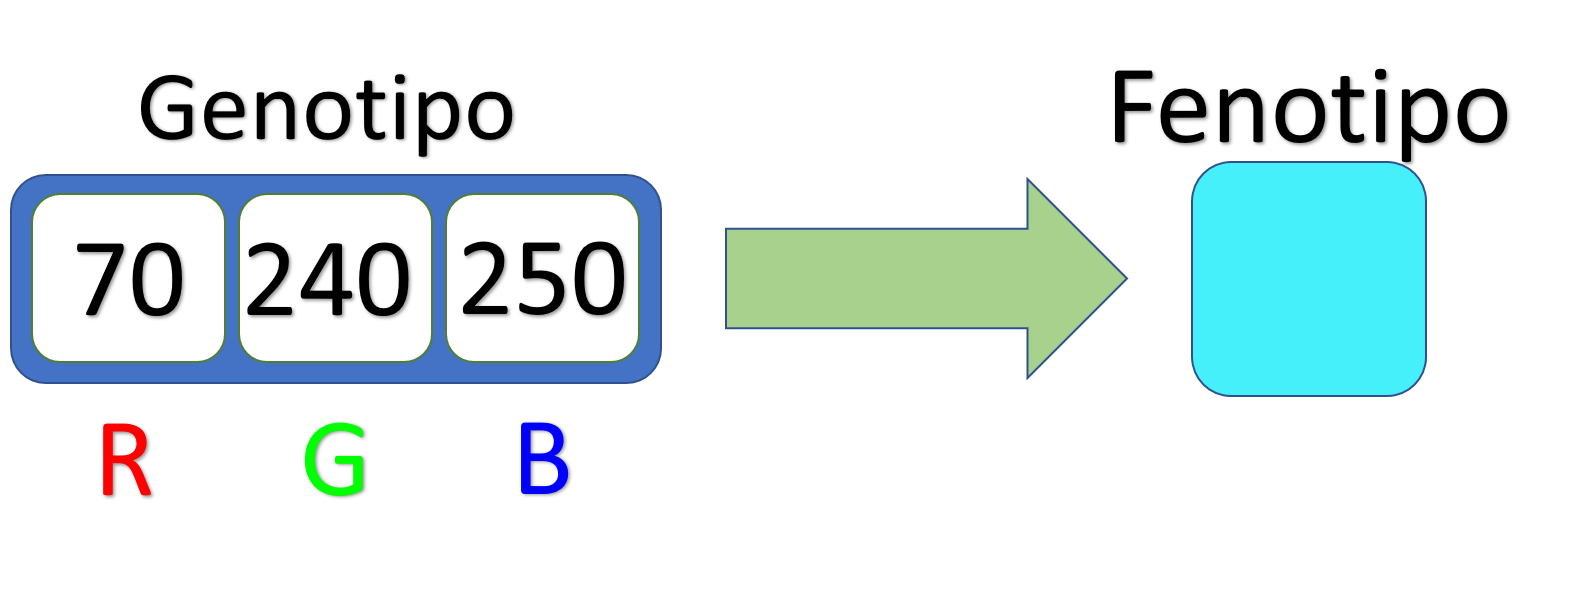
\includegraphics[width=0.6\textwidth]{genotipo-fenotipo}
\caption{Correspondencia genotipo-fenotipo.}
\end{figure}

Para la selección, recombinación y transformación de los individuos en el proceso de evolución se utiliza un mecanismo de selección y una serie de operadores genéticos \cite{cervigon09}:

\begin{itemize}
\item \textbf{Mecanismos de selección}: se encargan  de seleccionar un porcentaje de individuos de entre la población que eventualmente participarán de los procesos de cruce y mutación en esa generación. Hay distintos mecanismos de selección de individuos de los cuales dos de los más comunes son el de selección por ruleta y selección por torneo. La selección por ruleta consiste en dar una probabilidad de selección a cada individuo de la forma
\begin{equation*}
p_i = \frac{f(i)}{\sum\limits_{j=1}^n f(i)}
\end{equation*}
donde $f(i)$ es el valor \textit{fitness} del individuo $i$. Para cada individuo $i$ se define una puntuación acumulada de la forma
\begin{equation*}
q_i = \sum\limits_{j=1}^i p_j
\end{equation*}
A continuación se genera un número aleatorio $\alpha \in [0,1]$ y se selecciona el individuo $i$ que cumpla $q_{i-1} < \alpha < q_i$, este proceso se repite hasta seleccionar el porcentaje de individuos deseados. 

La selección por torneo consiste en elegir un conjunto de individuos al azar de la población, normalmente 2 ó 3 individuos, y seleccionar el individuo con mejor valor \textit{fitness}, este proceso se repite hasta seleccionar todos los individuos deseados.

\item \textbf{Operadores de cruce}: se encargan de cruzar los genotipos de los individuos seleccionados. El cruce se realiza entre dos individuos previamente seleccionados denominados padres que se cruzan y generan dos individuos nuevos denominados hijos. Al igual que los mecanismos de selección, existen muchos operadores  para cruzar los genotipos, pero estos operadores son dependientes de la codificación del genotipo. Si el genotipo es una cadena de enteros (codificación más común) el método de cruce más genérico es el cruce monopunto. Consiste en seleccionar aleatoriamente una posición idéntica en ambos genotipos de los padres (punto de corte) y generar dos hijos que conserven el mismo genotipo que su padre hasta la posición escogida y, a continuación, intercambiar la otra parte con la del otro padre.
\begin{figure}[H]
\centering
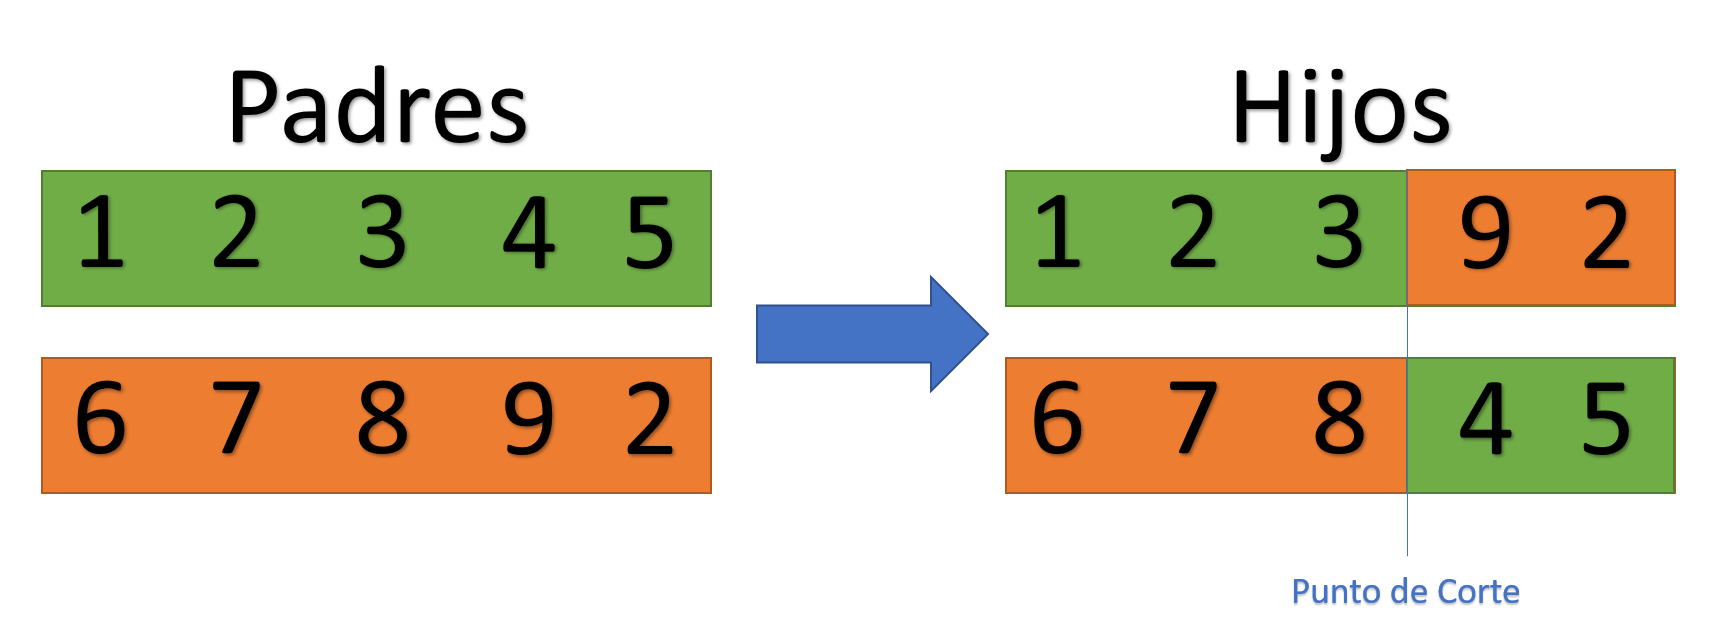
\includegraphics[width=0.7\textwidth]{operador-cruce}
\caption{Ejemplo de cruce monopunto.}
\end{figure}

\item \textbf{Operadores de mutación}: Estos operadores realizan cambios aleatorios en los valores del genotipo. Hay una gran variedad de operadores de mutación distintos y su posible uso, al igual que con los operadores de cruce, depende de la codificación del genotipo. En una representación del genotipo en forma de cadena de enteros el operador de mutación más utilizado es el operador de mutación aleatorio bit a bit (\textit{Integer Flip Mutation}) el cual recorre toda la cadena del genotipo y cambia un bit (o número) del genotipo por otro aleatorio dependiendo de una probabilidad.
\end{itemize}

Se pueden encontrar una gran variedad de algoritmos evolutivos, siendo algunos más recomendables que otros a la hora de abordar el problema que se quiere resolver o los resultados a obtener. Destacamos los siguientes:
\begin{itemize}
\item \textbf{Algoritmos genéticos}: los más comúnmente usados. En ellos el genotipo de los individuos es una cadena de números que posteriormente es decodificada para generar el fenotipo \cite{cervigon09}. Estos algoritmos usan los métodos de selección y operadores de cruce y mutación previamente explicados. 

\item \textbf{Programación genética}: se hacen evolucionar programas informáticos con el objetivo de encontrar el más óptimo para una tarea a realizar. La codificación de los programas en el genotipo es realizada mediante árboles en donde cada nodo representa un \textit{token} del lenguaje de programación escogido. Se explicarán con más detalle en la siguiente sección.

\item \textbf{Evolución gramatical}: similar a la programación genética pero usando cadenas de enteros como genotipo que dictan cómo se genera el código informático a través de una gramática independiente del contexto. Se explicará con más detalle posteriormente.
\end{itemize}

\section{Programación genética}
El objetivo de los algoritmos de programación genética es evolucionar programas informáticos escritos en un lenguaje determinado con el fin de encontrar el mejor programa que realice o resuelva un objetivo. En la programación genética el genotipo de los individuos es un árbol formado por nodos. Dependiendo de su contenido los nodos son nodos terminales (expresiones que no pueden ser expandidas, como números o variables) o nodos internos (normalmente representan funciones y contienen nodos hijos, por ejemplo un nodo interno que represente la suma entre dos números el cual tendrá dos nodos hijo donde la información obtenida de cada uno será un número). El fenotipo es el programa final que será ejecutado para evaluar al individuo y la forma de ser generado a partir del genotipo varía dependiendo del lenguaje en el que estén escritos los programas siendo algunos más complejos que otros. En algunos casos el fenotipo es igual al recorrido en inorden del árbol (genotipo) o en otros se necesitará realizar operaciones más complejas para generar el fenotipo \cite{cervigon09}.
\begin{figure}[H]
\centering
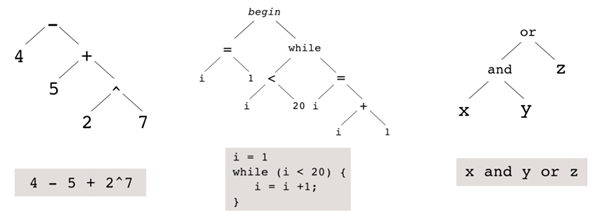
\includegraphics[width=0.9\textwidth]{genotipo-fenotipo-ejemplo}
\caption{Genotipo y fenotipo de distintos individuos \cite{colmenarApuntes}.}
\end{figure}

Existen distintos métodos para generar los individuos aleatorios de la población inicial:
\begin{itemize}
\item \textit{Grow}: se va eligiendo aleatoriamente nodos internos o nodos terminales, si se escoge un nodo terminal para una rama del árbol dicha rama se cierra y se prosigue con el resto de ramas abiertas. Si se elige un nodo interno se abren tantas ramas como indique el tipo de nodo y se expanden recursivamente siguiendo el mismo método hasta que todas las ramas hayan sido cerradas. Este método produce una población con árboles de profundidades irregulares.

\item \textit{Full}: se establece una profundidad máxima del árbol y se van generando nodos internos hasta que se alcanza la profundidad máxima momento en el que se elige únicamente nodos terminales hasta cerrar todas las ramas. Mediante este método la población generada se compone en su totalidad de individuos con árboles completos.

\item \textit{Ramped half-and-half}: método que usa ambos métodos anteriores, parte de la población es generada usando el método \textit{Full} y la parte restante mediante el método \textit{Grow}. El resultado es una mezcla de árboles irregulares de diferentes profundidades creadas por el método \textit{Grow} y árboles más regulares creados por el método \textit{Full}.
\end{itemize}

Los métodos de selección son los mismo que los usados en los algoritmos genéticos como selección por torneo o ruleta.
Como la codificación del genotipo ya no es una cadena de valores, los operadores de cruce y mutación comúnmente usados en los algoritmos genéticos (como el cruce monopunto) no pueden usarse y se emplean otros más específicos.

\blankline

El operador de cruce más usado en programación genética, denominado cruce de subárboles, consiste en elegir aleatoriamente en cada padre un punto de cruce (un nodo) y el subárbol que forma es intercambiado con el subárbol del otro padre.

\begin{figure}[H]
\centering
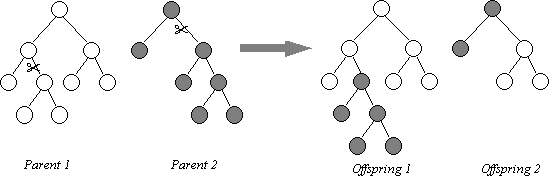
\includegraphics[width=0.9\textwidth]{cruce-subarboles}
\caption{Operador de cruce de subárboles \cite{tsang2000eddie}.}
\end{figure}

Existen distintos operadores de mutación para árboles, los más comunes son los siguientes:
\begin{itemize}
\item Mutación de subárbol: solo se aplica una vez por individuo. Selecciona un nodo aleatorio y sustituye todo su subárbol por uno nuevo generado aleatoriamente usando uno de los métodos nombrados anteriormente como \textit{Ramped half-and-half}.

\item Mutación puntual: elige un nodo aleatorio que cambia por otro nodo generado aleatoriamente (esto puede provocar cambios y conflictos en los subárboles del nodo mutado que han de ser arreglados).

\item Mutación terminal: un nodo terminal aleatorio se cambia por otro nodo terminal generado aleatoriamente.

\item Mutación de función: se selecciona un nodo interno de forma aleatoria y se cambia por otro nodo interno generado aleatoriamente pero que preserve las características del nodo anterior (mismo número de nodos hijo, función que devuelva un valor del mismo tipo, etc.).
\end{itemize}

La programación genética no está exenta de problemas y uno muy común es el \textit{Bloating}. Al realizar la operación de cruce, el árbol de los nuevos individuos generados pueden tener un tamaño excesivamente grande y que puede ir a más dado que este puede ser cruzado en generaciones posteriores (llegando a tener individuos con árboles extremadamente largos esparcidos por la población). Además, esto genera la aparición de intrones, grupos de nodos en el genotipo que generan trozos de código que no aportan nada a la funcionalidad del código generado y que intensifican la formación de \textit{Bloating}.

\begin{figure}[H]
\begin{lstlisting}[]
    ...
    if (distFantasmaMasCercano > 20) { 
        if (distFantasmaMasCercano < 10) {
            //Sección de programa que nunca llegará a ejecutarse
        }
    }
    ...
\end{lstlisting}
	\caption{Ejemplo de intrón.}
\end{figure}

Hay varios métodos para intentar solventar el problema del \textit{Bloating}:
\begin{itemize}
\item \textit{Naive}: se empeora el fitness precalculado de todos los individuos en la siguiente cantidad
\begin{equation*}
\textrm{Valor de empeoramiento del fitness} = k_{empeoramiento} * \textrm{tamano del árbol}
\end{equation*}
donde $k_{empeoramiento}$ es una constante previamente elegida. De este modo, los individuos con valores de \textit{fitness} similares pero con un genotipo más largo son penalizados frente a los individuos con genotipos más cortos.

\item \textit{Tarpeian}: trata de eliminar individuos que excedan la extensión media de la población en base a una probabilidad. Si un individuo con longitud de genotipo superior a la media ha sido elegido para su eliminación se le asigna el valor del peor \textit{fitness} posible de tal forma que en la siguiente generación este individuo tenga muy pocas probabilidades de ser seleccionado y se elimine.

\item \textit{Covariant Parsimony Pressure:} \cite{poli2008covariant} funciona igual que el metodo \textit{Naive} pero empleando un valor de $k_{empeoramiento}$ calculado en cada generación mediante una fórmula que tiene en cuenta características de los genotipos de la población, como su longitud media.
\end{itemize}

La programación genética ya ha sido utilizada para la evolución de un controlador del famoso juego Pac-Man. Koza \cite{koza1992genetic} utilizó la programación genética para evolucionar el código del controlador del personaje principal de Pac-Man de una versión personalizada del juego. Para ello empleó dos tipos de operadores, operadores de alto nivel para la obtención de información del juego (\textit{Distance-to-Pill},
\textit{If-Less-Than-or-Equal}) y operadores de acción (\textit{Advance-to-Food}). Con estos operadores el algoritmo construye y evoluciona el genotipo de los individuos guiándose por la función de fitness, que es básicamente el número total de puntos obtenidos por el Pac-Man antes de morir (obteniendo el fenotipo del individuo y ejecutandolo en el juego). Koza obtuvo resultados muy prometedores con este método.

Alhejali y Lucas \cite{alhejali2010evolving} realizan una implementación muy parecida a la de Koza pero usando operadores de un nivel más alto y abstracto (\textit{isInDanger()}, \textit{toSafety()}, ...) aunque obtuvieron resultados bastante similares. Sin embargo, Brandstetter y Ahmadi \cite{brandstetter2012reactive} optan por el uso de operadores de acción de bajo nivel (\textit{Up, Down, Left, Right}), obteniendo muy buenos resultados y realizando una comparativa con otros controladores evolucionados mediante programación genética (incluyendo los previamente nombrados). En la comparativa se aprecian mejores resultados con los operadores de bajo nivel que con los operadores de alto nivel o más abstractos.

\section{Gramáticas independientes del contexto}
Una gramática independiente del contexto (en adelante GIC o gramática) es una cuaterna formada por un conjunto de símbolos no terminales, un conjunto de símbolos terminales, un conjunto de reglas de producción (también denominadas expresiones) y un símbolo inicial. Mediante estos símbolos y reglas la gramática es capaz de generar un lenguaje independiente del contexto\cite{hopcroft_motwani_ullman_2007}\cite{HolgerApuntes}.

\textit{Backus-Naur Form} (BNF) es una notación formal para representar gramáticas independientes del contexto la cual es fácilmente interpretable por el ser humano. Una BNF se compone de símbolos terminales y no terminales (escritos entre \texttt{< >}). Estos símbolos no terminales pueden ser expandidos por una serie de producciones las cuales a su vez contienen un conjunto de símbolos no terminales o un terminal. La mayoría de lenguajes informáticos, por ejemplo, tienen una representación escrita en formato BNF \cite{garshol2003bnf}.

\begin{figure}[H]
\centering
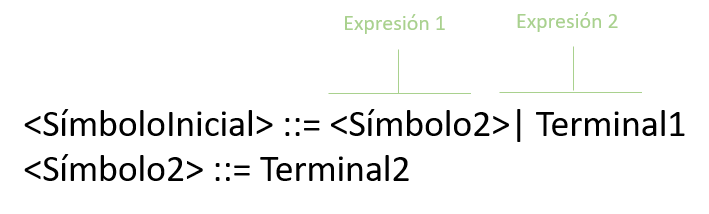
\includegraphics[width=0.45\textwidth]{bnf}
\caption{Ejemplo de BNF.}
\end{figure}

Para obtener una derivación (una secuencia de caracteres perteneciente al lenguaje que representa la BNF) se parte del símbolo inicial. A partir de aquí se repite recursivamente el siguiente proceso: se procesan todos los símbolos no terminales contenidos en la producción elegida. Para cada símbolo no terminal sin procesar se realiza el mismo proceso, se elige una producción perteneciente al mismo y se vuelve a realizar este proceso de forma recursiva hasta llegar a un símbolo terminal, momento en el que el símbolo no terminal se da por procesado y se pasa a procesar el siguiente símbolo no terminal sin haber sido completamente procesado. El proceso termina cuando todos los símbolos no terminales han sido procesados.

\begin{figure}[H]
\centering
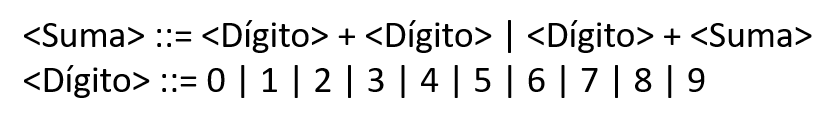
\includegraphics[width=0.5\textwidth]{bnf-ejemplo}
\caption{BNF que representa sumas de dígitos.}
\end{figure}

Para procesar y utilizar una BNF se usa un lector de BNFs que recorre y extrae información de la misma, como los símbolos y terminales que la componen.

\section{Evolución gramatical}
Evolución gramatical (\textit{Grammatical Evolution} en inglés) es un tipo de algoritmo evolutivo basado en la programación genética que permite generar automáticamente producciones o programas  con el objetivo de encontrar el óptimo que realice una acción o resuelva un problema. A diferencia de la programación genética, donde se utiliza un árbol para codificar el genotipo, en la evolución gramatical se usa un array de enteros como genotipo y una gramática independiente del contexto en notación \textit{Backus-Naur Form} (BNF) para la generación del fenotipo. Estos números enteros que componen el array del genotipo se denominan \textit{codones} y dictan qué producción perteneciente a una regla de la gramática se escoge a la hora de generar el fenotipo. Un ejemplo de genotipo formado por 5 codones tendría la forma: 37, 12, 5, 42, 1. El rango de valores que pueden tomar los codones se determina de antemano.

Para determinar la producción a procesar del símbolo no terminal siendo expandido se utiliza la siguiente fórmula:
\begin{equation}
\textrm{Producción a escoger} = \textrm{codón} \bmod \textrm{(nº de producciones para el símbolo a derivar)}
\end{equation}
donde $\bmod$ es la función de módulo entero. Esta fórmula devuelve un número que es la posición de la producción a seleccionar del símbolo no terminal que está siendo expandido \cite{o2012grammatical}.

\begin{figure}[H]
\centering
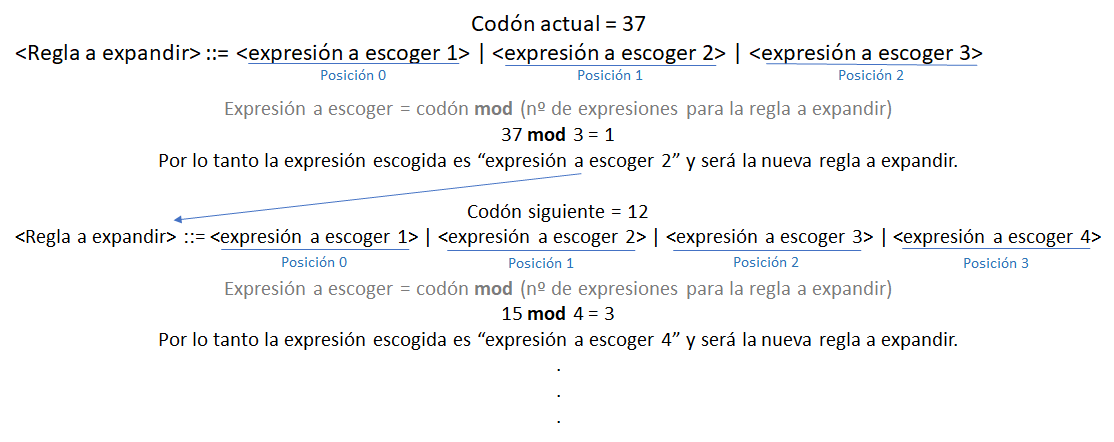
\includegraphics[width=\textwidth]{expandir-codon}
\caption{Ejemplo del proceso que se realizaría para transformar el genotipo mostrado anteriormente al fenotipo que representa.}
\end{figure}

Esta fórmula se aplica en orden a los símbolos no terminales hasta que todos hayan sido procesados, es decir, se hayan alcanzado en todos un símbolo terminal. A veces esto no se consigue con un único recorrido del genotipo, por lo que se realiza lo que se conoce como \textit{wrapping}, que consiste en  volver a empezar a leer el genotipo desde el principio y seguir expandiendo las reglas todavía sin expandir. El número de veces que se permite realizar \textit{wrapping} por individuo se determina de antemano y si, tras realizar \textit{wrapping} este número de veces no se ha conseguido derivar todos los símbolos, el individuo es descartado.

\begin{figure}[H]
\centering
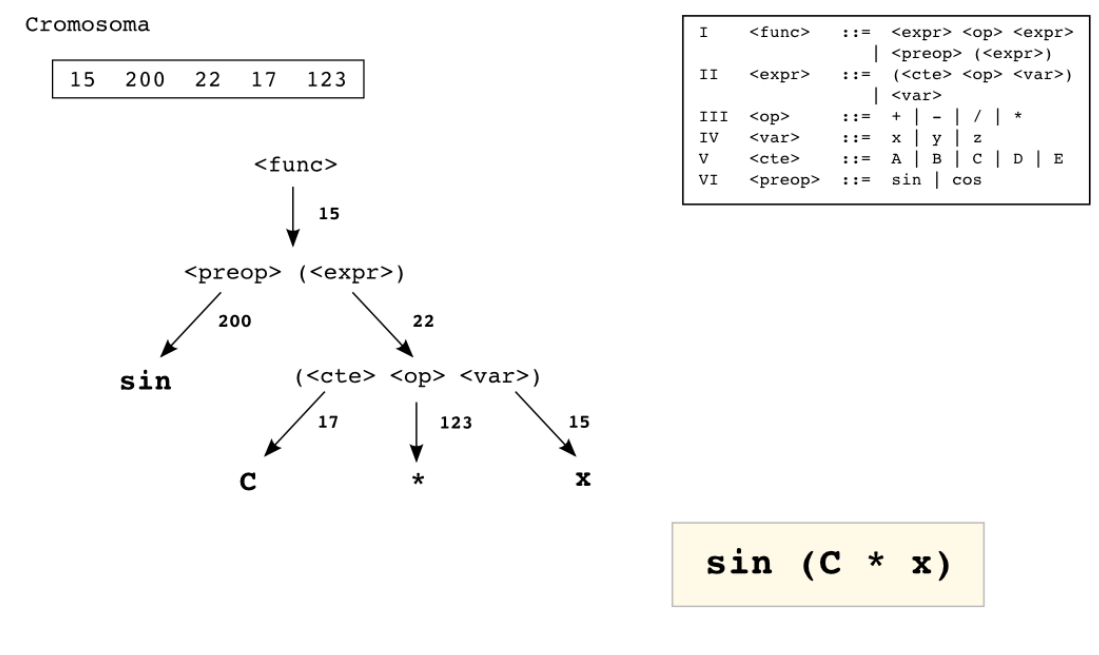
\includegraphics[width=\textwidth]{codon-a-arbol}
\caption{Conversión de un genotipo (cromosoma) a su fenotipo a través del método descrito anteriormente y utilizando la gramática dada \cite{colmenarApuntes}.}
\end{figure}

La estructura de partida de las también llamadas gramáticas evolutivas es muy similar a la de los algoritmos genéticos comunes.
\begin{enumerate}
\item Generar una población aleatoria.
\item Evaluar la población usando una función de fitness.
\item Cruzar la población mediante el operador de cruce elegido.
\item Mutar la población mediante el operador de mutación elegido.
\item Repetir desde el punto dos hasta que se alcance el número de generaciones.
\end{enumerate}

Sin embargo, el uso de operadores clásicos de cruce y mutación produce resultados poco óptimos debido a que genera poblaciones muy caóticas, un pequeño cambio en un codón del genotipo puede producir un programa completamente diferente y sin relación con el anterior dificultando en gran medida la convergencia de la población hacia el óptimo. Es por esta razón por la cual distintos operadores se han diseñado específicamente para su uso en gramáticas evolutivas.

La mayoría de las investigaciones se centran en los métodos de cruce debido a que son bastante destructivos (el fenotipo del hijo de dos padres suelen no tener ninguna relación con el fenotipo de sus padres lo que dificulta una evolución convergente). No es fácil dar con un nuevo método que mejore o no empeore el cruce monopunto, como es el caso del cruce homogéneo \cite{O'neill:2003:CGE:608284.608289}, pero hay algunos operadores de cruce que sí mejoran considerablemente el cruce monopunto e intentan minimizar el comportamiento destructivo que tiene el cruce en los algoritmos genéticos, como es el caso de \textit{LHS replacement crossover} \cite{harper2005structure}.

Este operador de cruce trata de cruzar dos individuos moviendo producciones enteras y no secuencias de codones arbitrarias. Para ello selecciona un codón aleatorio del genotipo y busca el símbolo que ha de ser expandido por ese codón a la hora de generar el fenotipo. Desde ese codón se cogen tantos codones como sea necesario para expandir completamente el símbolo (llegar a un símbolo terminal). Es este conjunto de codones el que es insertado en el genotipo del otro individuo y viceversa. Este proceso se puede ver como un ``cortar-pegar'' de trozos del fenotipo de un individuo en el fenotipo del otro individuo obteniendo hijos que poseen un fenotipo relacionado al del padre.

Los operadores de mutación pueden afectar de manera notable al fenotipo del individuo si se muta un codón que expande un símbolo no terminal. Así mismo puede generar mutaciones sin efecto si se genera un nuevo codón que tenga el mismo módulo que el anterior. Se suelen utilizar los operadores de mutación clásicos. Aún así, nuevos operadores de mutación han sido diseñados centrándose en gramáticas evolutivas, como por ejemplo la mutación neutral \cite{Oesch2015}. Este operador pretender dar mayor diversidad a la población, para ello muta aleatoriamente codones dándoles un nuevo valor que produzca el mismo módulo que el anterior al generar el fenotipo. Este cambio no afecta directamente al fenotipo (se mantiene igual) pero en las siguientes generaciones en las que el genotipo puede haber cambiado esta mutación neutral si puede tener efecto. Se puede utilizar en conjunto con otro operador de mutación que sí produzca cambios en el fenotipo, por ejemplo la mutación bit a bit.

Además de los operadores también se pueden encontrar cambios en la codificación del genotipo \cite{lourencco2016unveiling} o adaptaciones de distintos tipos de algoritmos genéticos a algoritmos de evolución gramatical con el fin de hacer esta misma más eficiente y efectiva, como es el caso de la evolución diferencial. La evolución diferencial es un algoritmo genético el cual genera una población auxiliar adicional y realiza el cruce entre elementos de la población auxiliar y la población principal. El operador de mutación en vez de generar cambios aleatorios utiliza individuos de la población y los combina mediante una fórmula matemática creando un nuevo individuo. El uso de este algoritmo aplicado a un genotipo-fenotipo del algoritmo de evolución gramatical da lugar al algoritmo denominado \textit{evolución diferencial gramatical} \cite{o2006grammatical}.

Otro método típicamente usado es el \textit{Grammatical Swarm Evolution} el cual es una mezcla de la evolución gramatical y \textit{Particle Swarm Optimization} (optimización por enjambre de partículas o PSO) \cite{o2004grammatical} \cite{gomez2010particle}. PSO es un algoritmo que intenta explorar todo el espacio de soluciones y así encontrar el máximo/mínimo global y no estancarse en máximos/mínimos locales. Para eso trata la población de individuos como partículas en un ``mapa'' (espacio de soluciones) representadas mediante una ``posición'' (estado actual) que cambia en cada generación dependiendo de la ``velocidad''  de la partícula. Esta ``velocidad'' se calcula en cada generación mediante una fórmula matemática que utiliza distintas variables como la ``posición'' de la mejor partícula actual (óptimo local) en el ``mapa''.

\blankline

Al igual que la programación genética, las gramáticas gvolutivas también han sido usadas previamente para la evolución de controladores de Pac-Man. Galván-López \cite{galvan2010evolving} usó una estrategia similar a la utilizada por Koza (en su implementación mediante programación genética) usando funciones de alto nivel para los operadores de movimiento (\textit{ANG - Avoid Nearest Ghost}) y para los operadores que obtienen información del estado del juego (\textit{avgDistBetGhosts}). Usaron una gramática compuesta por declaraciones \textit{if-else} para la elección del operador de movimiento adecuado basándose en ciertas características del estado actual del juego. Con esta implementación obtuvieron resultado similares a los controladores obtenidos mediante programación genética y con la ventaja que la gramática utilizada se puede cambiar con facilidad (añadiendo o quitando reglas) y obteniendo de este modo distintos comportamientos adaptados a las nuevas funciones disponibles.

Liberatore \cite{Liberatore2014} propuso otra implementación interesante pero esta vez para el controlador de los fantasmas, utilizando gramáticas evolutivas y \textit{Flocking Strategies} para obtener comportamientos y estrategias basados en una inteligencia de colmena.

\section{Algoritmos Evolutivos Multiobjetivo}
Todas las distintas ramas de algoritmos evolutivos que hemos presentado anteriormente comparten la característica de que están enfocados a optimizar  un único objetivo en la  función de \textit{fitness}. Sin embargo, a veces aparecen problemas en los que se buscan soluciones que optimicen más de una variable y se les denomina problemas multiobjetivo.

Si por cada objetivo a optimizar se crea una función fitness para determinar cómo de bueno es el individuo respecto a ese objetivo entonces se busca:
\begin{equation*}
Optimizar \{f_i(X) \mid \forall i = 1, \dots, \textrm{nº de objetivos}\}
\end{equation*}
donde $f_i$ es la función $i$-ésima de \textit{fitness}.

Por ejemplo, un algoritmo evolutivo que determine dónde invertir en bolsa podría tener dos objetivos, maximizar las ganancias de la inversión y minimizar el riesgo de pérdidas.

La dificultad de un algoritmo multiobjetivo es determinar el óptimo global, es decir, el individuo que optimiza de la mejor forma todos los objetivos. La solución al ejemplo anterior no es trivial ni única, pues el algoritmo puede dictar una inversión que optimice el beneficio obtenido pero con un alto riesgo de pérdidas así como una inversión segura pero que genera muy pocos beneficios.

\blankline

Se suele emplear la definición de óptimo en un contexto multiobjetivo dada por Vilfredo Pareto, denominado óptimo de Pareto. Se dice que una solución Y domina (es mejor) a otra X si es igual o mejor en todos los objetivos y es estrictamente mejor en al menos un objetivo \cite{cervigon09}.
\begin{figure}[H]
\begin{equation*}
f_i(y) \leq f_i(x), (\forall i = 1, \dots, \textrm{nº de objetivos}\}) \wedge \exists f_i(y) < f_j(x)
\end{equation*}
\caption{Óptimo de Pareto para un problema de minimización.}
\end{figure}

Normalmente (como en el ejemplo anterior de inversión en bolsa) existen varios óptimos de Pareto, es decir, un conjunto de soluciones que dominan al resto pero que entre ellas no se dominan. A este conjunto de soluciones se le denomina \textit{frente de Pareto}.

\begin{figure}[H]
\centering
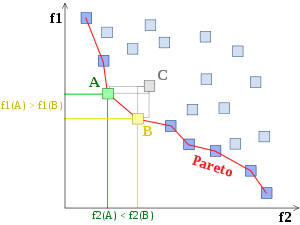
\includegraphics[width=9cm]{pareto}
\caption{Frente de Pareto de un conjunto de soluciones para un problema de minimización. C es una solución dominada por A y B, ambas pertenecientes al frente de Pareto \cite{pictPareto}.}
\end{figure}

A la hora de implementar un algoritmo multiobjetivo podemos elegir entre diferentes  métodos. El más sencillo, y que no altera los esquemas clásicos de los algoritmos evolutivos, es el denominado multiobjetivo mediante funciones agregativas que consiste en la creación de una función fitness $f$ como una combinación lineal de funciones en donde cada una representa un objetivo a optimizar.
\begin{equation*}
f(x) = \theta_1f_1(x) + \theta_2f_2(x) + \dots + \theta_nf_n(x)
\end{equation*}
donde $\theta_i$ son coeficientes utilizados para dar más o menos peso a cada función. El principal problema de este enfoque a problemas multiobjetivo es la dificultad para encontrar los pesos adecuados.

Un método muy utilizado es el desarrollado por Deb, \textit{et al.} denominado NSGA-II (\textit{Non-dominated Sorting Genetic Algorithm}) el cual ofrece buenos resultados pero es bastante exigente computacionalmente, sobretodo para poblaciones grandes \cite{deb2002fast}. El método consiste en la identificación de los distintos frentes de Pareto de la población en la generación actual. Para ello se identifican los individuos pertenecientes al frente de Pareto de la población y se les asigna rango uno, nuevamente se vuelve a identificar el frente de Pareto de la población sin tener en cuenta los individuos que pertenecen al frente de Pareto ya identificado y se les asigna rango dos y se realiza este proceso hasta que todos los individuo de la población tienen asignado un frente de Pareto al que pertenecen. Para los individuos de cada frente de Pareto se calcula una serie de valores denominados \textit{distancias de saturación} respecto a los distintos objetivos. Usando estas distancias de saturación la selección se realiza mediante el método de torneo, se escogen dos elementos aleatorios de la población y se selecciona el que pertenezca al menor frente de Pareto (rango más bajo). Si ambos individuos pertenecen al mismo frente de Pareto entonces se escoge el que tenga mayor distancia de saturación.

\subsection{JECO}
Como punto de partida para abordar el uso de gramáticas evolutivas hemos decidido emplear el \textit{framework} JECO \cite{jecoGit} (\textit{Java Evolutionary Computation Library}). Inicialmente se valoraron otras opciones como  GEVA \cite{gevaGit}, reutilizar código nuestro o partir de cero.

JECO (Java Evolutionary COmputation) es un framework de inteligencia artificial orientado a la computación evolutiva, creado por José Luis Risco Martín y José Manuel Colmenar Verdugo, con la colaboración posterior de Josué Pagán Ortiz.

Soporta muchas técnicas de programación evolutiva, entre las que nos interesaron las gramáticas evolutivas simples y multiobjetivo (utilizando el algoritmo NSGA-II descrito anteriormente y que utilizaremos en nuestro trabajo), con soporte para el uso de varios hilos de procesamiento.

\chapter{Ms. Pac-Man}
\begin{figure}[H]
\centering
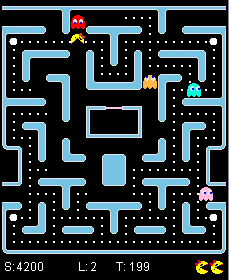
\includegraphics[width=6.5cm]{pacman}
\end{figure}

Ms. Pac-Man es un juego antológico desde su aparición en los arcades en el año 1981. Desde entonces han sido muchas las variantes de este clásico y sus diversos usos (recreacional, investigación, competición).
 
La versión del juego que vamos a utilizar, ``\textbf{\textit{Ms. Pac-Man Vs. Ghosts}}''\cite{pacmanvsghostsTournamentPage}\cite{pacmanvsghostsGit}, está implementada por Philipp Rohlfshagen, basada en implementaciones previas de Simon Lucas y David Robles, los tres de la universidad de Essex, Reino Unido.


\section{Descripción del juego}
Las variantes del juego difieren mucho en cuanto a objetivos de juego y recompensas por los mismos, así como reglas a seguir. La descripción de la versión \textit{Ms. Pac-Man Vs. Ghosts} es la siguiente:

El jugador o Pac-Man debe recorrer laberintos comiendo ``\textit{pills}'' y enfrentándose a cuatro fantasmas que intentarán perseguir a Pac-Man. Se dispone de 4 laberintos, todos con un ``\textit{lair}'' donde nacen y resucitan (cada nivel más rápidamente) los cuatro fantasmas tras ser comidos, y un punto con las mismas características para Pac-Man, el cual puede moverse por los laberintos cambiando su dirección en cualquier momento, siempre que la entrada dada por el jugador sea un movimiento válido (en otro caso continúa hacia delante en la dirección del último movimiento realizado exitosamente).
 
\blankline

Los laberintos son una serie de pasillos y cruces de caminos, repletos de \textit{pillsi}, y con cuatro ``\textit{power pills}'' cada uno. Las pills proporcionan puntos, y las power pills (con forma de pill agrandada) además permiten a Pac-Man comerse a los fantasmas durante un breve periodo de tiempo.

Todos los laberintos tienen una estructura toroidal (o \textit{wraparound}, esto es, al salir de los límites por un lado se aparece por el contrario, dando continuidad y dinamismo a la partida). Al comer Pac-Man una \textit{power pill}, puede comerse a los fantasmas durante un breve periodo de tiempo (siendo este periodo más corto en cada nivel), enviandolos al lair y ganando puntos. Además, durante la duración del efecto de las power pills, la velocidad de los fantasmas queda reducida a la mitad de la de Pac-Man. Las \textit{pills} y las \textit{power pills} también dan puntos, y se pasa al siguiente nivel cuando no queda ninguna de ambas.
 
No existen las frutas de la versión original del juego que aportan puntos adicionales.
Pac-Man tiene tres vidas (La inicial y dos más en reserva), pudiéndose obtener vidas adicionales cada 10.000 puntos.

Además, si tras 4000 iteraciones de la partida aún quedan \textit{pills} o \textit{power pills}, se pasa al siguiente nivel (considerando una iteración un intervalo de tiempo en el que tanto los fantasmas como Pac-Man hacen su movimiento y se actualiza el estado del tablero de juego). Este límite de tiempo se diseñó para evitar, en competiciones previas, que si un participante diseñaba una inteligencia artificial para controlar a los fantasmas, estos no pudieran bloquear una región del laberinto indefinidamente.
 
Los fantasmas tratan de impedir a Pac-Man completar cada laberinto y, al moverse (cuando no son comestibles) a la misma velocidad que este, emplean estrategias basadas en su superioridad numérica. Además, los fantasmas no pueden darse la vuelta (retroceder), con una excepción: turno a turno se evalúa con resultado aleatorio la posibilidad de obligar a todos los fantasmas a darse la vuelta, por defecto 0.015\%.
 
La puntuación se obtiene con los siguientes cálculos (originales del código de competición):
\begin{itemize}
\item Comer pill: 10 puntos.
\item Comer power pill: 50 puntos.
\item Comer fantasma: 200 puntos, duplicándose el valor por cada fantasma comido en cadena (Si durante la duración de la misma \textit{power pill} se come un segundo fantasma, este vale 400; el siguiente 800, etc).
\end{itemize}

\section{Arquitectura para crear bots}
El código del juego viene preparado para facilitar a los concursantes diseñar sus bots, que han de implementar su código en la clase ``\textit{pacman/entries/pacman/MyPacMan.java}'', con la posibilidad de añadir clases auxiliares en ``\textit{pacman/entries/pacman/}''. Dicha clase incluye el método a implementar, que ha de devolver el siguiente movimiento de Pac-Man en cada turno, pudiendo hacer consultas a las funciones de la clase ``\textit{Game.java}'', que contiene el estado del juego para realizar el más conveniente en cada caso.
 
La versión original trae como ejemplo una serie de controladores para los fantasmas, que vamos a usar para medir la ``calidad'' o ``cómo de buenos'' son los programas que generemos con gramáticas evolutivas. Son los siguientes:
\begin{itemize}
\item \textbf{Random Ghosts}. Los fantasmas toman direcciones aleatorias cada vez que llegan a una intersección y al salir del \textit{lair}.

\item \textbf{Starter Ghosts}. Versión de los fantasmas que consiste en: Alejarse de Pac-Man si está cerca de una \textit{power pill} o si el fantasma en concreto es comestible (por haberse comido Pac-Man una \textit{power pill} mientras él estaba vivo), o si no, con un 90\% de posibilidades dirigirse hacia Pac-Man y con un 10\% hacer un movimiento aleatorio entre los que sean posibles para el fantasma en ese momento.

\item \textbf{Aggressive Ghosts}. Cada vez que un fantasma llega a una intersección tiene una probabilidad determinada de o bien dirigirse hacia Pac-Man, o bien hacer un movimiento aleatorio.

\item \textbf{Legacy}. \textit{Legacy} diferencia entre los 4 fantasmas. Cada vez que llegan a una intersección, tres de ellos siempre se dirigen hacia Pac-Man por el camino más corto, cada uno con un cálculo de distancia diferente: Manhattan, Euclídea y utilizando unas distancias precalculadas para cada dos posiciones de cada laberinto. El cuarto fantasma hace siempre un movimiento aleatorio.

\item \textbf{Legacy 2: The Reckoning}. La versión más compleja y efectiva de fantasmas junto a \textit{Legacy}. Tienen en cuenta situaciones como estar muy agrupados entre sí para poder dispersarse, o alejarse de Pac-Man si son comestibles (\textit{edibles}) o Pac-Man está cerca de una \textit{power pill}. Las distancias para determinar los movimientos son definibles mediante constantes en la clase del código.
\end{itemize}
 
También trae dos controladores para Pac-Man, uno que hace movimientos aleatorios (similar a \textit{Random Ghosts}) y otra con un intento primitivo de estrategia que tiene en cuenta si los fantasmas cercanos son comestibles o no y plantea la posibilidad de atacarlos.

\section{Competiciones}
El framework descrito se ha utilizado y se utiliza actualmente para organizar competiciones en las que los participantes implementan un bot para Pac-Man o para los fantasmas, y tratan de obtener la mayor puntuación posible dadas una serie de reglas.
 
Actualmente activa, la ``\textit{Ms. Pac-Man Vs. Ghost Team Competition}'' fue celebrada en el CIG2016\cite{CIG2016Page} (\textit{Computational Intelligence \& Games 2016}) y va a ser celebrada de nuevo en 2017. En esta competición se utiliza la regla de ``observación parcial'', en la que tanto Pac-Man como los fantasmas sólo pueden obtener información de lo que está en su rango de visión, es decir, el pasillo del mapa en el que estén o, si están en una intersección, los pasillos que se originen de ella.

\chapter{Bots basados en secuencias de acciones} \label{cap:bots-secuencia-acciones}
En primer lugar y una vez decididos nuestros dos frameworks de partida, fue necesaria la integración entre el código de Pac-Man y JECO para poder empezar a realizar experimentos.

\section{Integración de Ms. Pac-Man y JECO}
\begin{figure}[H]
\centering
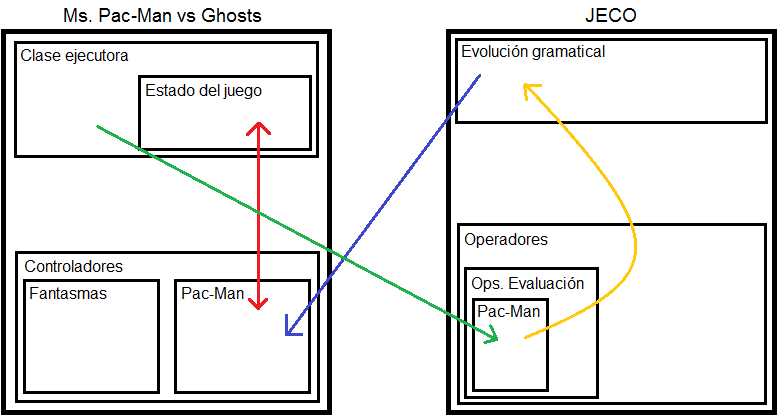
\includegraphics[width=\textwidth]{integracion-jeco-pacman}
\caption{Diagrama de la integración de Pac-Man y JECO.}
\end{figure}
\begin{itemize}
\item Flecha azul: JECO evoluciona individuos (en la primera generación son aleatorios) y transmite su fenotipo al framework de Pac-Man, para ser evaluados.

\item Flecha roja: El controlador de Pac-Man suministra movimientos a la clase ejecutora, al tiempo que la clase ejecutora transmite información necesaria al controlador para que este pueda determinar qué movimientos hacer.

\item Flecha verde: El framework de Pac-Man transmite a una función de evaluación especializada para Pac-Man en JECO la información de la partida (en primer lugar empezamos transmitiendo únicamente la puntuación obtenida).

\item Flecha amarilla: La función de evaluación para Pac-Man traduce la información resultante de la partida a un fitness, que es transmitido al proceso de evaluación gramatical. El individuo evaluado adquiere un fitness y en función del mismo se condiciona la siguiente generación (junto a los resultados del resto de individuos).
\end{itemize}

Debido a que JECO persigue encontrar individuos con el fitness más bajo posible (minimización), tenemos la necesidad de emplear fitness en los que se considere mejor el menor o adaptarlo a maximización. Optamos por lo primero, y empleamos como fitness inicial:
\begin{equation*}
f = 100000 - score
\end{equation*}
donde $score$ es la puntuación total que conseguimos y $100000$ es una cota máxima a dicha puntuación.


\section{Idea general}
Empezamos por plantearnos los objetivos más sencillos e indispensables:
\begin{itemize}
\item Gramáticas evolutivas mono-objetivo.
Un solo thread.

\item Una sola función de fitness que tuviera únicamente en cuenta los puntos conseguidos (Recibiendolos JECO tras cada evaluación del árbol de derivación obtenido en Pac-Man).

\item Uso de una gramática que solo permitiese generar programas en forma de cadena de movimientos simples (\textbf{\texttt{U D L R}}) como una sucesión de caracteres.

\item Un generador de trazas minimalista para registrar los fenotipos que producían una mejora del fitness durante la ejecución.
\end{itemize}

Partiendo de un sistema de evolución gramatical que devolvía árboles de derivación en forma de cadenas de caracteres, la idea inicial fue encapsular tanto acciones como observadores del estado del juego dentro de dichas cadenas, que contendrían de manera prefijada las acciones a realizar o evaluar por el controlador de Pac-Man, repitiéndose en un bucle la evaluación de los caracteres de la cadena desde el principio de la misma al llegar al final. Dicha cadena-programa puede verse como un autómata en las que las transiciones son la evaluación de un carácter y paso al siguiente.

\section{Un primer bot}
La primera versión de autómata conseguido encadenaba los distintos movimientos posibles (\texttt{Arriba, Abajo, Derecha, Izquierda}, \textbf{\texttt{U D L R}} respectivamente) pertenecientes a un alfabeto inicial que más tarde fuimos ampliando y mejorando durante la implementación.
 
El controlador de Pac-Man generaba una transición en el autómata secuencialmente al tiempo que este le proporcionaba el movimiento asociado al estado al que transitaba, volviendo el autómata al estado inicial cuando finalizaba la cadena de caracteres definidos por la gramática. El fundamental problema de este sistema es que el bot no tiene en cuenta el estado de juego, viéndose obligado a realizar acciones de la secuencia que tal vez sean contraproducentes.
 
Por ejemplo, para una de nuestras más sencillas gramáticas de partida:
\begin{lstlisting}[frame=single, breaklines=no, basicstyle=\fontsize{10}{11}\ttfamily, caption=Gramática básica para encadenar movimientos.]
    <mov> ::= <mov> U  | 
              <mov> D  | 
              <mov> R  | 
              <mov> L  |
              U | 
              D | 
              R |
              L
\end{lstlisting}

Una derivación gramatical válida podría ser: ``\textbf{\texttt{U R D L}}'', que podría verse como un autómata con la siguiente forma \cite{jflapPage}:
\begin{figure}[H]
\centering
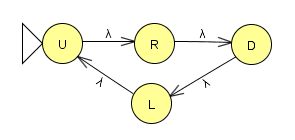
\includegraphics[width=8cm]{jflapo}
\caption{Autómata correspondiente al código \texttt{U R D L}}
\end{figure}

El controlador consume un símbolo tras otro transitando al siguiente estado del autómata al mismo tiempo, traduciéndose en este caso en un comportamiento que lleva a Pac-Man a intentar dar vueltas en sentido horario.
 
Sorprendentemente únicamente con esto, al ser los laberintos siempre los mismos, conseguía hacer algunos puntos antes de ser aniquilado por los fantasmas, pese a la precariedad del método. Lo relevante en este punto era que teníamos una primera integración que funcionaba.
 
A continuación se muestra el resultado de uno de los primeros experimentos realizados, con tamaño de población 100, 50 generaciones, una evaluación por individuo, selección por Torneo Binario, cruce monopunto con 60\% de probabilidad de cruce e \textit{Integer flip mutation} con 10\% de probabilidad de mutación. El controlador de fantasmas era \textit{Starter ghosts} (nuestro bot aún no tenía ninguna oportunidad contra \textit{Legacy}).
\begin{table}[H]
\centering
\begin{tabular}{cc}
\hline
\textbf{Fenotipo} & \textbf{Puntos (avg)} \\ \hline
\texttt{LLDLDRLD}          & 2480                  \\ \hline
\end{tabular}
\end{table}

\section{Incorporando condicionales y acciones de alto nivel}
Para dotar al autómata de capacidad de decisión que tuviera en cuenta el estado del juego en el que se encontraba el bot, incluimos \textbf{símbolos condicionales}, que siempre iban precedidos del símbolo ``\texttt{?}''. A su vez el símbolo ``\texttt{?}'' siempre iba precedido de un carácter que representaba la condición a evaluar.
Si una condición evaluada resultaba cierta, se realizaba la \textbf{acción} que definía el carácter ubicado a continuación del de la condición. Si no, se omitía. 

\blankline

La versión final disponía de evaluaciones y acciones de alto nivel especificados por la cadena de instrucciones del autómata, cuyo alfabeto era el siguiente:
\begin{table}[H]
\centering
\begin{tabular}{ccc}
\hline
\textbf{Char} & \textbf{Tipo de símbolo} & \textbf{Comportamiento}                     \\ \hline
P             & condicional              & Condicional de fantasma no comestible cerca \\
B             & condicional              & Condicional de fantasma comible cerca       \\
H             & acción                   & Huir                                        \\
E             & acción                   & Comer pill                                  \\
W             & acción                   & Comer powerpill                             \\
F             & acción                   & Comer fantasma                              \\ \hline
\end{tabular}
\end{table}

La gramática diseñada para hacer uso de este lenguaje, tenía la siguiente forma:
\begin{lstlisting}[frame=single, breaklines=no, basicstyle=\fontsize{10}{11}\ttfamily, caption=Gramática con acciones de alto nivel.]
    <expr>   ::= ? <cond> <expr> | <action> <expr> | <action>
    <cond>   ::= P | B
    <action> ::= H | E | W | F
\end{lstlisting}

\subsection{Fenotipos producidos}
En bots producidos por esta implementación a veces se aprecia un atisbo de primera inteligencia muy primitiva, así como los habituales intrones o fragmentos de programa inútiles.
 
Los siguientes fenotipos fueron obtenidos tras experimentos con tamaño de población 100, 50 generaciones, una evaluación por individuo, selección por Torneo Binario, cruce monopunto con 60\% de probabilidad de cruce e \textit{Integer flip mutation} con 10\% de probabilidad de mutación. Los fantasmas siguen siendo \textit{Starter ghosts} en esta etapa, dados los malos resultados obtenidos contra fantasmas \textit{Legacy}.
\begin{table}[H]
\centering
\begin{tabular}{cc}
\hline
\textbf{Fenotipo} & \textbf{Puntos (avg)} \\ \hline
\texttt{E?P?PH}          & 6580                  \\
\texttt{?B?PE?BHEHE}          & 7000                  \\ \hline
\end{tabular}
\end{table}

Como ejemplo, la traducción a pseudocódigo del primer programa sería lo siguiente:
\begin{lstlisting}[frame=single, breaklines=no, basicstyle=\fontsize{10}{11}\ttfamily, caption=Pseudocódigo correspondiente al programa \texttt{E?P?PH}]
    MIENTRAS (true)
        Ir hacia la pill más cercana
        SI (fantasma no comible cerca) ENTONCES
            SI (fantasma no comible cerca) ENTONCES
                Huir del fantasma no comible más cercano
            FIN SI
        FIN SI
    FIN MIENTRAS
\end{lstlisting}

Que se traduce en ir siempre hacia la pill más cercana, salvo que haya un fantasma no comible cerca de Pac-Man, en cuyo caso se aleja de él. Se aprecia una doble evaluación consecutiva de lo mismo que no aporta nada: Un problema típico en programación genética. 

\blankline

Resulta destacable el descubrimiento por parte de los bots generados mediante este sistema de la variable ``\textit{Global reversal}'', que en cada movimiento asigna a los fantasmas una probabilidad aleatoria muy baja de darse todos la vuelta.
 
Los fenotipos consistentes en comer pills y huir cuando haya un fantasma cerca, producen una estrategia en la que el bot de Pac-Man huye a la vez que agrupa la mayoría de fantasmas detrás de él. Cuando ocurre el susodicho \textit{Global reversal}, los fantasmas cambian su dirección a la opuesta, y dado que no pueden cambiarla de nuevo salvo que ocurra otro global reversal y las distancias son calculadas teniendo esta limitación en cuenta, todos pasan a estar ``lejos'' de Pac-Man y este puede comer pills con seguridad.
\begin{figure}[H]
\centering
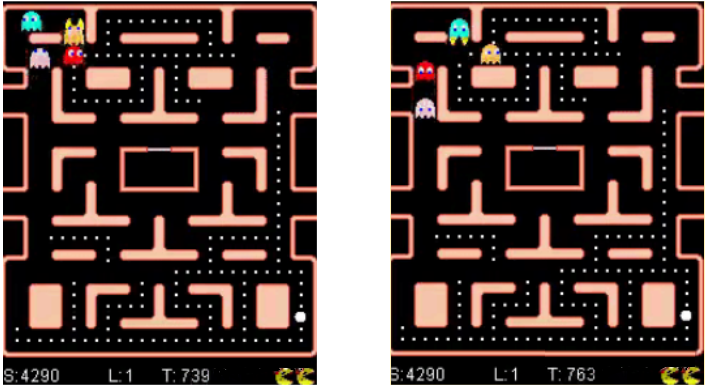
\includegraphics[width=0.8\textwidth]{global-reversal}
\caption{\textit{Global reversal} de los fantasmas.}
\end{figure}

\section{Limitaciones}
Tal como esperábamos, el empleo de este ingenuo autómata tiene varias limitaciones.
 
El funcionamiento de nuestros condicionales permitía una sola condición, es decir, no nos permitían evaluar varias premisas (usando operadores lógicos binarios y/o unarios) salvo mediante el encadenamiento de condicionales (\texttt{if}). 
Tampoco teníamos la posibilidad de emplear una segunda acción que solo se ejecutase en caso de no cumplirse el condicional, a modo ``\texttt{else}''. Además, solo se realizaba una acción en el consecuente, en lugar de poder realizar una serie de acciones. 
 
Otra limitación era la imposibilidad de construir estrategias con continuidad temporal debido a la ejecución de la cadena de instrucciones de forma lineal, dado que esta era única para toda la ejecución y simplemente se volvía a empezar por el principio tras llegar al final.
 
Además, este funcionamiento en forma de bucle que repite la misma secuencia de acciones podía provocar muy fácilmente la ejecución de una acción sin sentido en el contexto en el que el juego se encontraba en determinado momento.
 
Previamente decidimos comprobar si era posible adaptar el autómata con el que contábamos en ese momento de forma que se solventase los problemas descritos.
 
Para dicha prueba, introdujimos un nuevo estado de huida (similar a un estado trampa, pero con una vía de salida), en el que se entraba en caso de encontrarse algún fantasma (comible) por debajo de un radio de peligro. 
En este estado de huida se codificaba un comportamiento, en alto nivel y ajeno al funcionamiento normal del autómata, en el que permanecía hasta que Pac-Man estuviera fuera de la distancia de peligro. Tras estar fuera de peligro, el bot salía del estado de huida y seguía ejecutando la cadena de instrucciones dada por el autómata en el punto en el que se encontraba antes de entrar al estado de huida.
\begin{figure}[H]
\centering
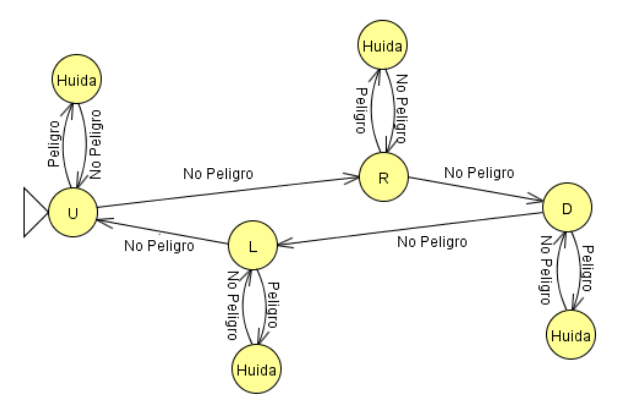
\includegraphics[width=0.8\textwidth]{prueba-automata}
\caption{Ejemplo de autómata que usa el estado Huida.}
\end{figure}

A través de esta prueba comprobamos que la escalabilidad del autómata no era realista, ya que suponía la codificación de eventos cada vez más complejos de gestionar debido a la aparición de conflictos con los ya introducidos a la hora de controlar las transiciones.
 
Llegados a este punto y con esos problemas, considerábamos seriamente la posibilidad de realizar una nueva implementación alejada del sistema de autómatas de movimientos concatenados.

\chapter{Bots basados en árboles de decisión} \label{cap:bots-arboles}

\section{Idea general}
Un Árbol de Decisión es un tipo especial de árbol utilizado en el área de Inteligencia Artificial cuyos nodos internos representan condiciones a evaluar y sus nodos hoja representan las acciones a realizar, resultados, soluciones, etc. El recorrido de un Árbol de Decisión es sencillo, se empieza por el nodo raíz y se evalúa su condición, dependiendo del resultado de esta evaluación se elige el siguiente nodo (hijo del nodo evaluado) que será evaluado y así sucesivamente hasta que se encuentre un nodo hoja.
\begin{figure}[H]
\centering
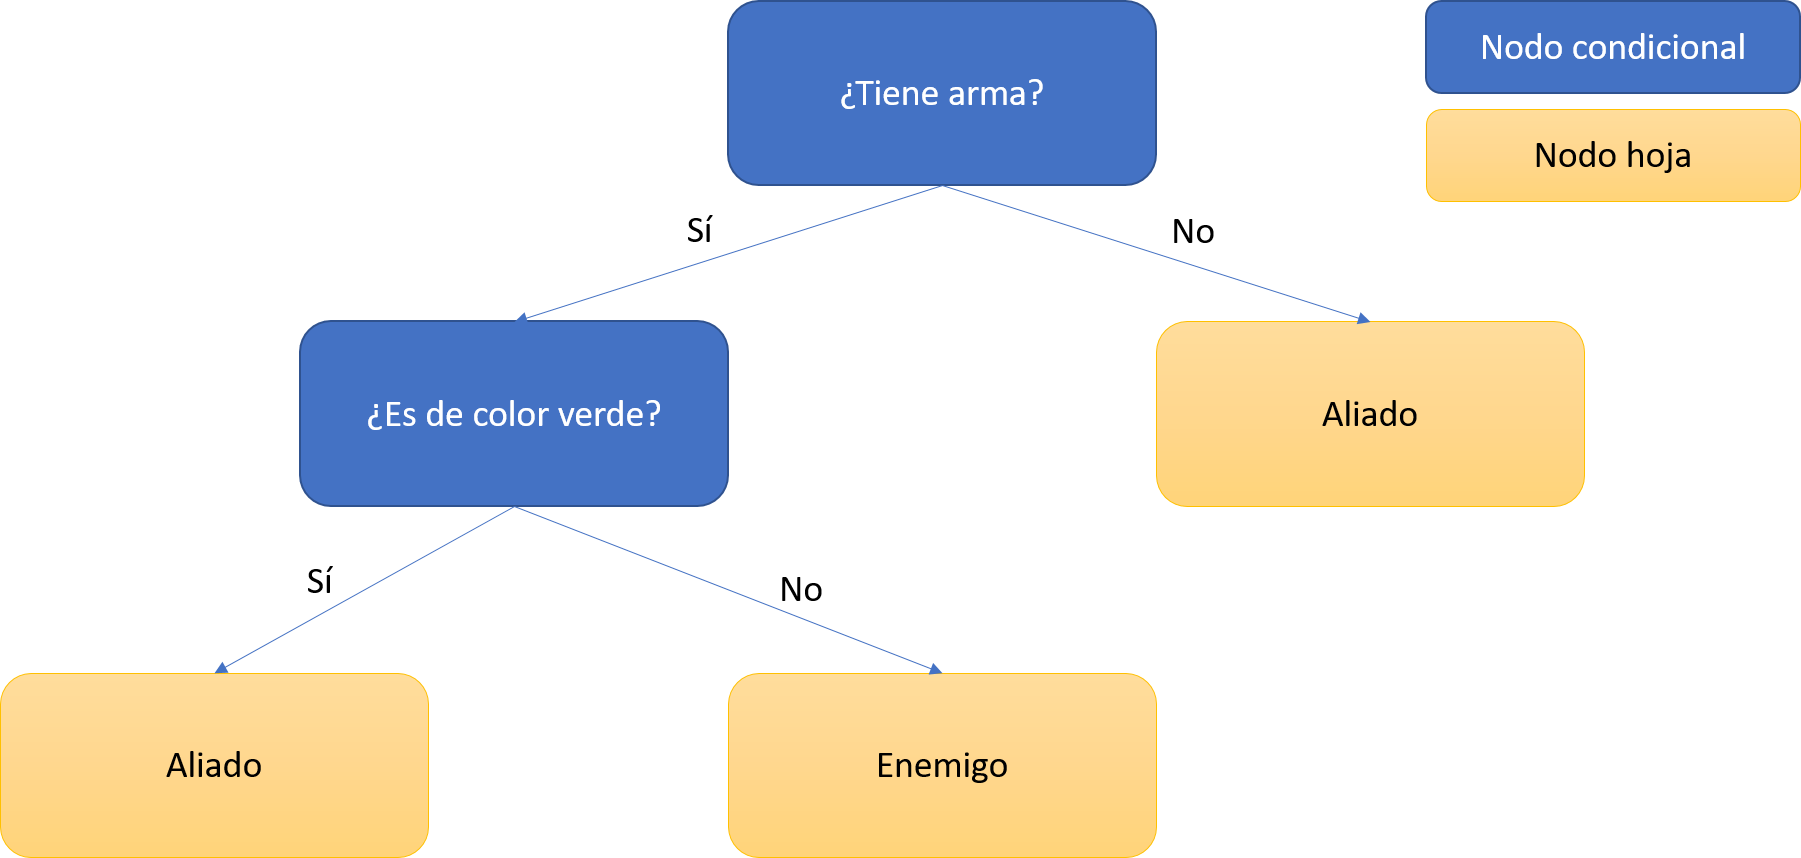
\includegraphics[width=\textwidth]{arbol-decision}
\caption{Árbol de decisión para determinar si un individuo es enemigo o aliado.}
\end{figure}

Los Árboles de Decisión suelen emplearse ampliamente en áreas donde sean necesarias decisiones deterministas automatizadas como finanzas, estadística, videojuegos, aprendizaje automático, etc. Son fáciles de entender y muy rápidos de procesar una vez construidos \cite{aihorizonDecisiontrees}.

En esta fase optamos por seguir un nuevo enfoque mediante Inteligencia Artificial Reactiva. Esto significa evaluar en cada turno un árbol de decisión (partiendo siempre desde la raíz), comprobando una serie de condiciones del estado de la partida, y a partir de ellas determinar una única acción a realizar. La decisión de seguir este enfoque persigue que nuestros bots resultantes tengan un comportamiento con continuidad dentro de una misma situación pero a la vez sean capaz de adaptarse a cambios repentinos en el estado del juego. 
 
Por ejemplo,a partir del código:
\begin{lstlisting}[caption=Ejemplo de código]
    if ( getDistanceToClosestNonEdibleGhost >= 4 ){
        getDirectionToClosestEdibleGhost
    } else {
        getDirectionAwayFromClosestNonEdibleGhost
    }
\end{lstlisting}

construiríamos el siguiente árbol:
\begin{figure}[H]
\centering
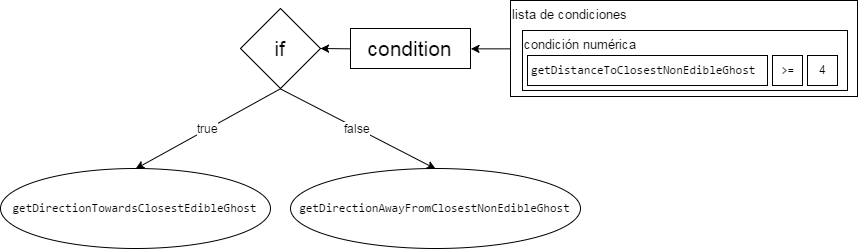
\includegraphics[width=\textwidth]{codigo-a-arbol}
\caption{Árbol contruido a partir de ejemplo de código.}
\end{figure}
La ejecución de este árbol consistiría en turno a turno evaluar desde el nodo raíz: primero, comprobar si la distancia al fantasma no comible más cercano es menor o igual que 4. En caso de que sea así, evalúa la rama izquierda recursivamente, y al ser esta un nodo hoja ejecuta la acción determinada por este, en este caso acercarse al fantasma comible más cercano. En caso de la que condición no se cumpla, se ejecutará de forma análoga la rama derecha, tratándose de un nodo hoja con la acción que genera un movimiento de huida del fantasma más cercano. 

\subsection{Árboles de decisión}
Posteriormente optamos por un cambio en la representación del fenotipo. Concretamente, a partir de cada fenotipo generado por el algoritmo evolutivo, generamos un árbol de decisión para simplificar significativamente la ejecución de una partida con dicho fenotipo, y así lograr la ya mencionada Inteligencia Artificial Reactiva. Dicho árbol contiene las diferentes funciones para consultar el estado de juego (los nodos no terminales) y para decidir movimientos (nodos terminales) como enumerados, obteniéndose cada movimiento evaluando recursivamente el árbol.
 
La razón de estos árboles era poder codificar comportamientos mucho más complejos en sus diferentes ``ramas'', pudiendo además explotar la riqueza de las gramáticas, simplificar la lógica de ejecución, y desarrollar una base mucho más estable sobre la que apoyar futuras iteraciones.

\subsection{Parsing de fenotipo a árbol}
A la hora de realizar el cambio estructural de fenotipo, optamos por realizar un parsing del fenotipo desde una cadena de caracteres (producida por JECO mediante evolución gramatical) a un árbol que organiza los ya mencionados condicionales, consecuentes y movimientos de la forma más intuitiva posible. La estructuración de dichos elementos dentro del árbol se realiza de la siguiente forma:

\subsubsection{Nodos terminales}
Los nodos terminales realizan una acción o una consulta. Si es una acción puede tratarse de:
\begin{itemize}
\item Movimientos simples (direccionales)
\item Movimientos basados en información del juego. Por ejemplo, ``el movimiento que aleja más a Pac-Man del fantasma más cercano''
\end{itemize}

En el caso de las consultas al estado del juego, estas pueden devolver distancias en formato entero (distancia al fantasma comible más cercano, ...) o booleanos (¿Está Pac-Man en una intersección?, ...).

\subsubsection{Nodos condicionales}
Los nodos condicionales contienen una lista de parámetros booleanos (los cuales hemos denominado condiciones) y otra lista que indica qué operadores booleanos binarios operan dichos parámetros. En caso de tratarse de un \texttt{if}, contendrá un nodo hijo con un consecuente, y en caso de ser un \texttt{else}, dos.
 
Una condición puede ser de varios tipos, según el tipo de los parámetros que contenga:
\begin{itemize}
\item de función booleana
\item de función numérica, operador numérico (binario) y función numérica
\item de función numérica, operador numérico (binario) y número
\item de número, operador numérico (binario) y función numérica
\end{itemize}

Los parámetros de tipo función que contenga una condición una vez más se trataran de enumerados, con la diferencia de que en este caso el método que poseen indicará el valor (booleano o numérico) de la consulta del estado de alguna variable de la partida. Finalmente, una condición puede encontrarse negada.

\subsection{Adaptador de árbol a movimiento de Pac-Man}
Para poder ejecutar partidas con estos árboles de decisión, necesitamos implementar un nuevo controlador de Pac-Man. Este controlador contiene el árbol de derivación, actuando como wrapper, de forma que con cada solicitud de movimiento realizada al controlador, este evalúa el árbol de forma recursiva, hasta encontrar un nodo terminal que devuelva un movimiento y que cumple todas sus condiciones previas.

Nótese  que la evaluación de dichos condicionales supone la evaluación de numerosos parámetros booleanos y enteros evaluados entre sí. Estos parámetros son obtenidos directamente de consultas al estado de la partida.

Finalmente se obtiene un movimiento, bien generado por la acción de un nodo terminal a través de la llamada a una determinada función interna del juego Ms. Pac-Man vs Ghosts, bien realizando un movimiento simple direccional.

\section{Gramáticas desarrolladas}
Todas nuestras gramáticas producen códigos basados en inteligencias artificiales reactivas, es decir, a cada turno de movimiento (denominado internamente como \textit{tick}) se evalúan una serie de condiciones del estado del tablero para producir un único movimiento de forma no ambigua. Las gramáticas diseñadas usan una estructura de anidamientos de declaraciones \texttt{if-else} que posteriormente un \textit{parser}\footnote{Un parser es una herramienta que mediante el uso de una gramática transforma texto escrito en el lenguaje representado por la gramática a una representación interpretable por otro sistema \cite{parserTechopedia}.
} convertirá a un Árbol de Decisión. Este Árbol de Decisión tendrá una traducción directa de las funciones escritas en la Gramática a funciones interpretables por el bot (escritas en \textit{Java}) que serán ejecutadas en el proceso de evaluación.
 
A la hora de desarrollar gramáticas las dividimos en tres categorías dependiendo del tipo de acciones que pueden producir:
\begin{itemize}
\item Bajo nivel: Son gramáticas cuyos nodos terminales, aquellos que dicen al bot de Pac-Man qué movimiento hacer en cada \textit{tick} del juego, se constituyen únicamente de las funciones \texttt{Up, Down, Left, Right} que son una codificación directa de las teclas de movimiento que dispondría un humano al jugar el juego.

\item Medio nivel: En lugar de las funciones básicas de movimiento (\texttt{Up, Down, ...}), disponen de funciones de un nivel medio,  entendiéndose nivel medio como funciones que dictan una acción directa, como puede ser comerse la \textit{pill} más cercana, huir del fantasma más cercano, ir a por la \textit{power pill} más cercana, etc.

\item Alto nivel: Se diferencian de las de medio nivel en que sus funciones terminales son muy abstractas y no se puede determinar directamente qué dirección o comportamiento tomará el bot, estas funciones son del estilo de \textit{comer, huir, atacar, ...} funciones que se entienden cuál es su objetivo pero que pueden realizarse de distintas maneras.
\end{itemize}

\subsection{Parámetros del experimento realizado} \label{sec:params}
Todos los resultados de esta sección han sido obtenidos empleando los mismos operadores, parámetros y probabilidad con la que se emplean los operadores del algoritmo evolutivo para permitir una comparación objetiva del rendimiento empleando diferentes gramáticas. Estos parámetros son:
\begin{table}[H]
\centering
\begin{tabular}{lc|c|}
\cline{3-3}
\textbf{}                                                                & \multicolumn{1}{l|}{\textbf{}}     & \multicolumn{1}{l|}{\textbf{Porcentaje}} \\ \hline
\multicolumn{1}{|l|}{\textbf{Población}}                                 & 100                                & -                                        \\ \hline
\multicolumn{1}{|l|}{\textbf{Generaciones}}                              & 100                                & -                                        \\ \hline
\multicolumn{1}{|l|}{\textbf{Evaluaciones por individuo}}                & 30                                 & -                                        \\ \hline
\multicolumn{1}{|l|}{\textbf{Longitud cromosoma}}                        & 100                                & -                                        \\ \hline
\multicolumn{1}{|l|}{\textbf{Límite superior codón\footnotemark[2]}} & 256                                & -                                        \\ \hline
\multicolumn{1}{|l|}{\textbf{Método de selección}}                       & Torneo Binario\footnotemark[3] & -                                        \\ \hline
\multicolumn{1}{|l|}{\textbf{Método de cruce}}                           & LHS                                & 60                                       \\ \hline
\multicolumn{1}{|l|}{\textbf{Método de mutación}}                        & Integer Flip                       & 10                                       \\ \hline
\multicolumn{1}{|l|}{\textbf{Mutación Neutral}}                          & Sí                                 & -                                        \\ \hline
\multicolumn{1}{|l|}{\textbf{Elitismo}}                                  & Sí                                 & 5                                        \\ \hline
\end{tabular}
\caption{Parámetros utilizados.}
\end{table}
\footnotetext[2]{valor máximo que puede tomar}
\footnotetext[3]{o NSGA II si se está empleando multiobjetivo}

\subsection{Gramática de bajo nivel}
Con la gramática de bajo nivel pretendemos que el bot tenga un comportamiento basado en estímulos muy específicos y utilizando solo los operadores de movimiento de los que un jugador humano dispone (\texttt{moveup, moveDown, moveRight, moveLeft}). Como son operadores de bajo nivel que no disponen de información del juego (\textit{pill} más cercana, posición de fantasmas, etc), la gramática necesita contener una gran cantidad de funciones que devuelvan información del estado actual del juego:
\begin{itemize}
\item \texttt{getDistanceToClosestNonEdibleGhost}: Devuelve la distancia al fantasma peligroso más cercano.

\item \texttt{getDistanceToClosestNonEdibleGhost{Up, Down, Left, Right}}: Distancia al fantasma peligroso más cercano a la posición del bot en la dirección dada.

\item \texttt{getDistanceToClosestEdibleGhost}: Devuelve la distancia al fantasma comestible más cercano.

\item \texttt{getDistanceToClosestEdibleGhost{Up, Down, Left, Right}}: Distancia al fantasma comestible más cercano a la posición del bot en la dirección dada.

\item \texttt{getNumberOfActivePowerPills}: Devuelve la cantidad de \textit{power pills} que se encuentran actualmente en el tablero.

\item \texttt{getDistanceToClosestPill}: Distancia a la \textit{pill} (también considerando las \textit{power pills}) más cercana independientemente de la orientación del bot.

\item \texttt{getDistanceToClosestPill{Up, Down, Left Right}}: Devuelve la \textit{pill} más cercana al bot en la dirección especificada.

\item \texttt{getClosesPowerPill{Up, Down, Left Right}}: Idéntica a las anteriores pero teniendo en cuenta solo las \textit{power pills}.

\item \texttt{getClosestJunctionExitsNumber{Up, Down, Left, Right}} = Número de salidas de la intersección más cercana a la posición del bot en la dirección dada.

\item \texttt{getDistanceToClosestJunction{Up, Down, Left, Right}} = Distancia del bot a la intersección más cercana dada una dirección.

\item \texttt{getClosestNonEdibleGhostDistanceToClosestJunction{Up, Down, Left Right}}: Devuelve la distancia del fantasma peligroso más cercano a la intersección más cercana al bot en la dirección dada.

\item \texttt{getClosestEdibleGhostDistanceToClosestJunction{Up, Down, Left Right}}: Identica a las anteriores funciones pero con fantasmas comestibles.

\item \texttt{getGeometricMeanDistanceToNonEdibleGhosts}: Devuelve la distancia media geométrica a los fantasmas peligrosos.

\item \texttt{getGeometricMeanDistanceToEdibleGhosts}: Idéntica a la anterior pero la distancia a los fantasmas comestibles.
\end{itemize}

Los resultados de estos operadores de obtención del estado del juego se comparan dentro de las condiciones de las declaraciones \texttt{if} contra un número. Este número en vez de permitir generarlo de forma arbitraria por la gramática lo que hemos decidido es introducir nosotros un conjunto discreto de números que pueden ser escogidos para las comparaciones, reduciendo de este modo el espacio de búsqueda y la generaciones de números absurdos (extremadamente grandes).

\subsubsection{Notación BNF}
\begin{lstlisting}[caption={Gramática de bajo nivel.}]
<grammar> ::= <selection-statement>
 
<selection-statement> ::= if( <condition> ){ <statement> }
                          else{ <statement> }
                        | if( <condition> ){ <statement> }
 
<statement> ::= <terminal-func>
              | <selection-statement>
 
<terminal-func> ::= <simpleMoves>
 
<condition> ::= <number-func> <number-operator> <number>
 
<number-func> ::= getDistanceToClosestNonEdibleGhost
                | getDistanceToClosestNonEdibleGhostUp
                | getDistanceToClosestNonEdibleGhostDown
                | ... 
 
<number-operator> ::= ==
                    | !=
                    | <
                    | >
                    | <=
                    | >=
 
<simpleMoves> ::= moveUp
                | moveDown
                | moveLeft
                | moveRight
 
<number> ::=  5 | 10 | 15 | 20 | 25 | 30
           | 40 | 50 | 60 | 75 | 80 | 90
\end{lstlisting}

\subsubsection{Resultados}
\begin{figure}[H]
\centering
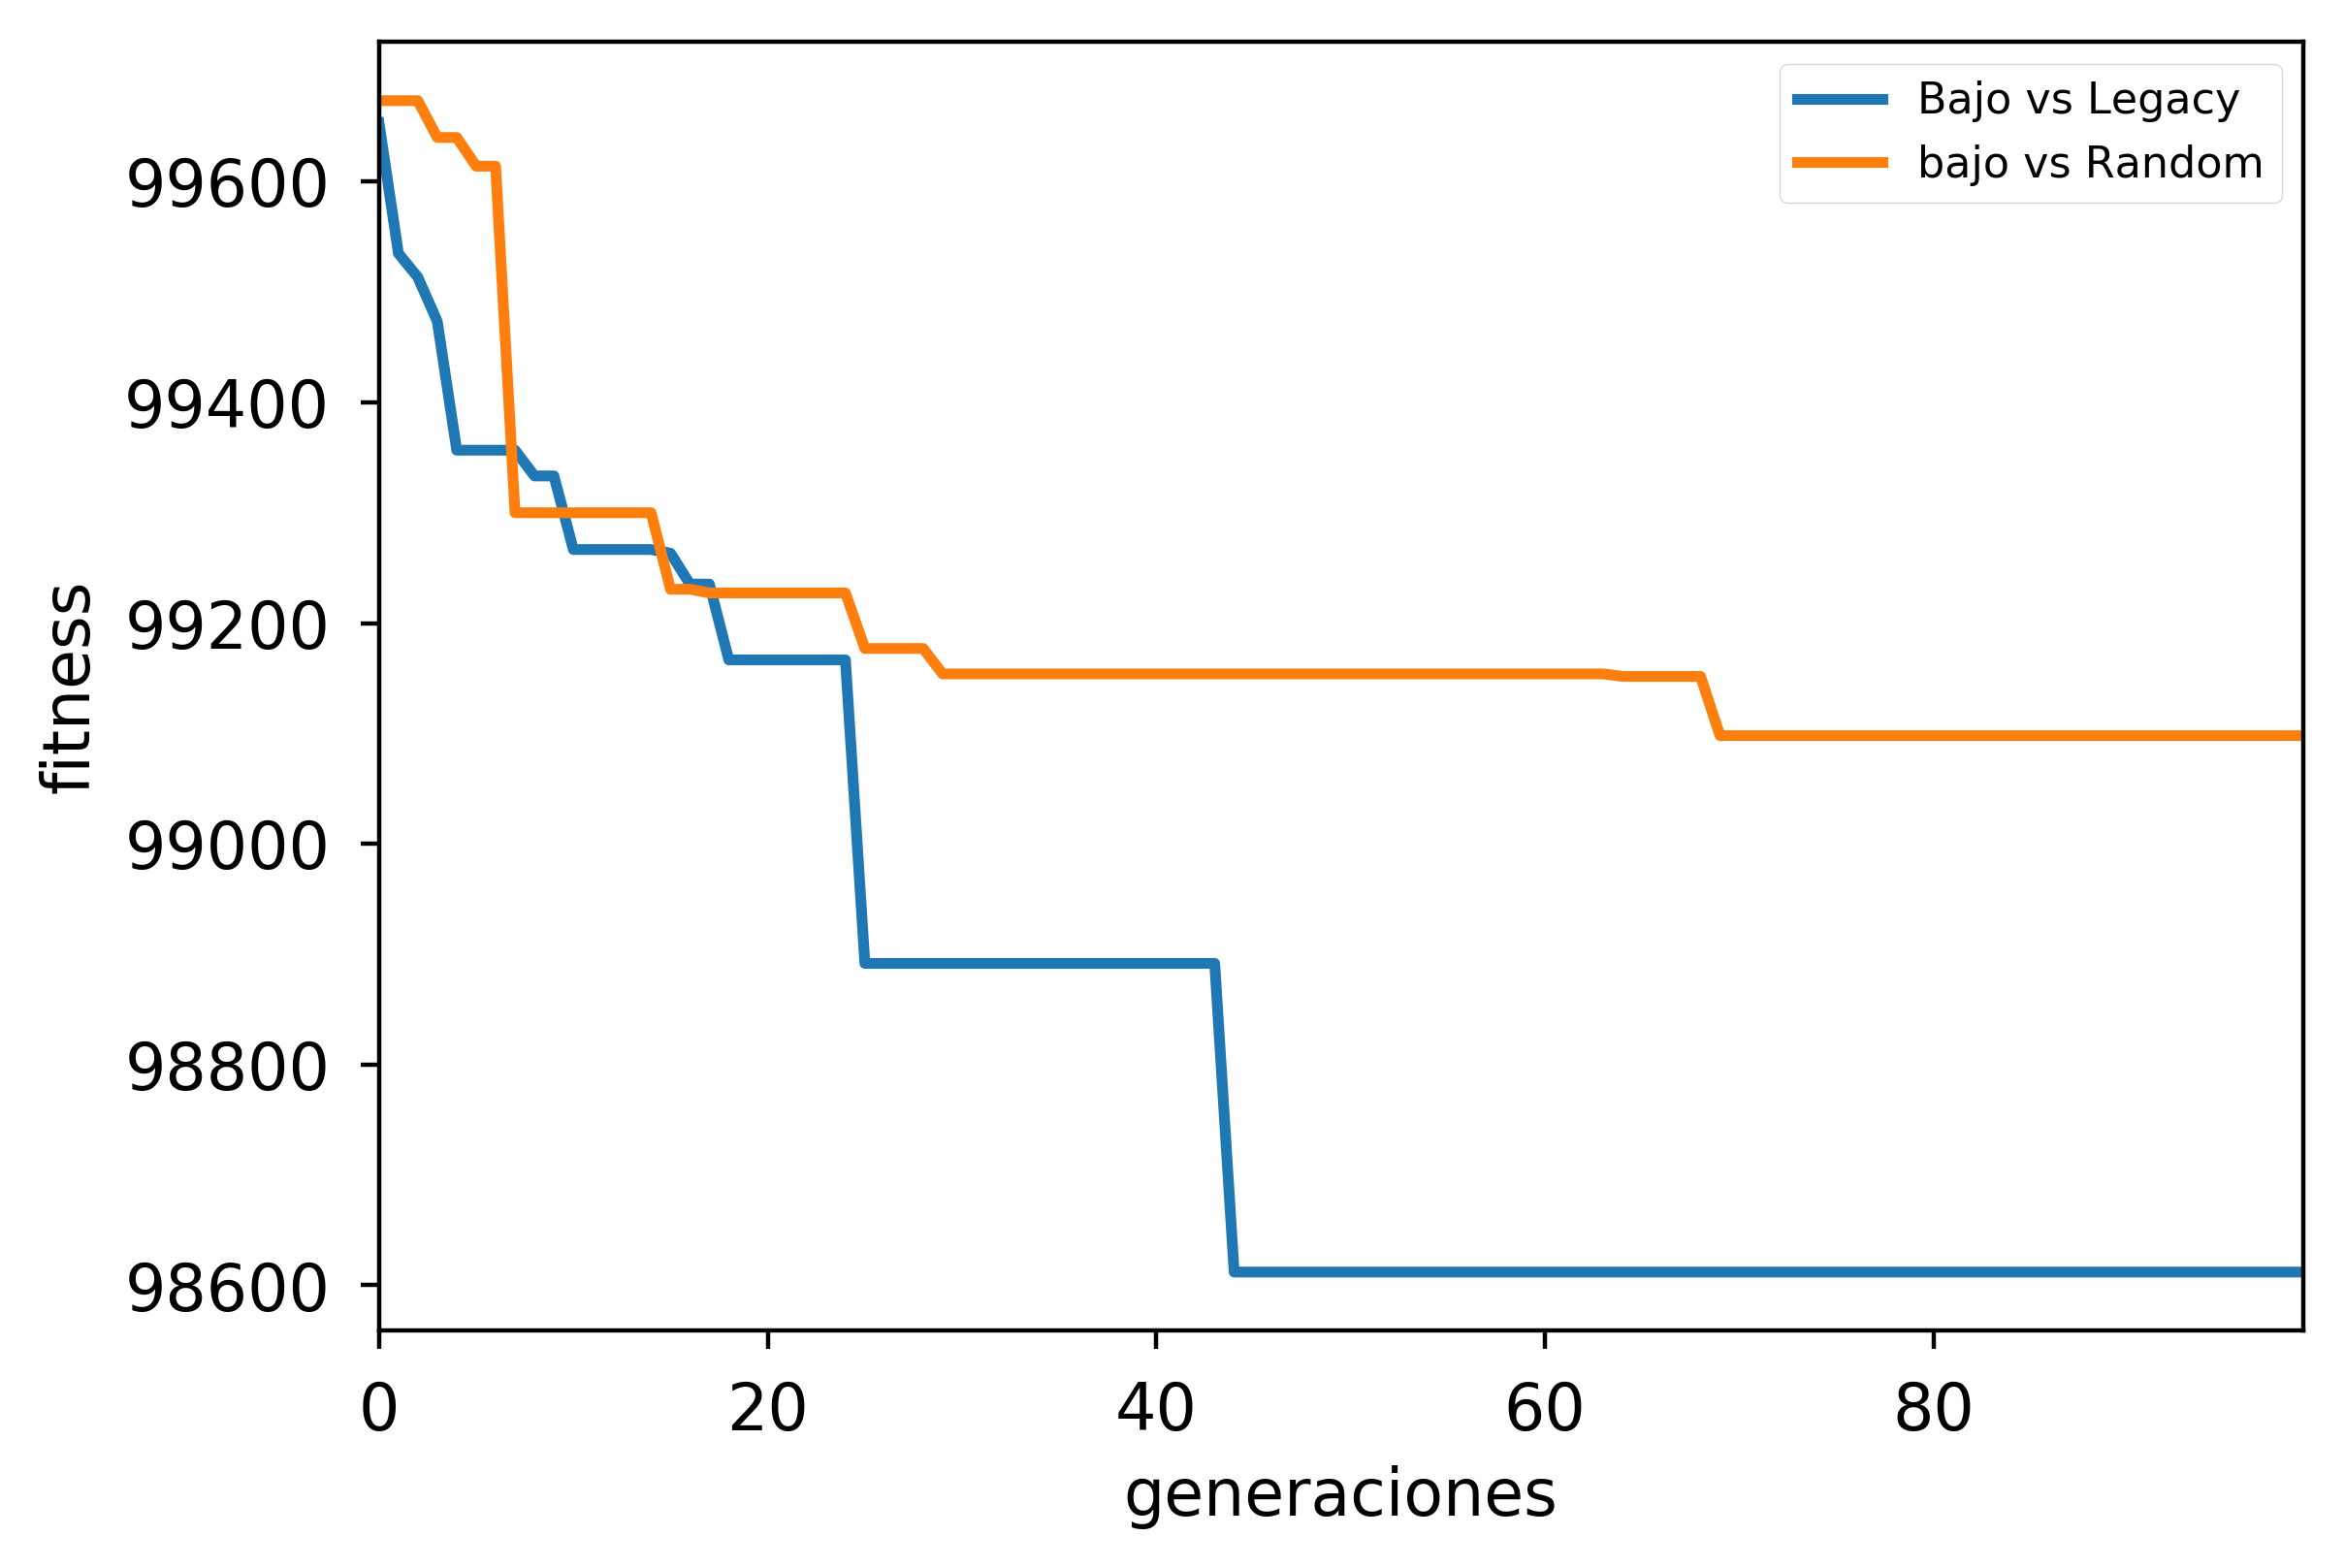
\includegraphics[width=0.8\textwidth]{grafica/low_level}
\caption{Gráfica que muestra las primeras 100 generaciones de dos ejecuciones distintas contra los controladores de fantasmas Random y Legacy usando la gramática de bajo nivel. Función fitness: 1000000 - puntos obtenidos.}
\end{figure}

Se obtuvieron las siguientes conclusiones a través de distintas ejecuciones:
\begin{itemize}
\item Los programas generados (fenotipo) son bastante largos debido a que hay muchos anidamientos de \texttt{if-else} que generan distintas acciones para determinados casos particulares. Esto es un resultado esperado al usar la gramática de bajo nivel.

\item Se obtienen malos resultados en cuanto a puntos obtenidos pero hay una gran convergencia de la población hacia el individuo óptimo actual.

\item El comportamiento del mejor individuo es siempre el mismo. Pac-Man va directamente a la esquina inferior izquierda del nivel y se queda quieto en cierto punto en el cual los fantasmas no le detectan, consiguiendo pasarse niveles porque el juego cada 4000 \textit{ticks} cambia de nivel inexorablemente y da una cierta cantidad de puntos al jugador. Este error del juego solo lo detecta hasta el nivel 3, nivel en el que es siempre eliminado por los fantasmas. A este comportamiento le hemos denominado bot ``Camper''.
\end{itemize}

\begin{lstlisting}[caption={Ejemplo de bot típico producido usando la gramática de bajo nivel entrenado contra Random Ghosts.}]
if (getDistanceToClosestNonEdibleGhostUp != 25) {
  if (getDistanceToClosestNonEdibleGhostLeft <= 90) {
    moveRight
  } else {
    if (getDistanceToClosestJunctionLeft <= 10) {
      if (getClosestEdibleGhostDistanceToClosestJunctionRight < 20) {
        if (getDistToClosestPowerPillUp < 30) {
          moveLeft
        } else {
          if (getDistanceToClosestNonEdibleGhostDown > 25) {
            moveRight
          } else {
            moveRight
          }
        }
      } else {
        if (getGeometricMeanDistanceToNonEdibleGhosts < 10) {
          moveLeft
        } else {
          if (getClosestJunctionExitsNumberLeft > 20) {
            if (getNumberOfActivePowerPills > 90) {
              if (getClosestJunctionExitsNumberUp != 10) {
                moveLeft
              }
            }
          } else {
            moveUp
          }
        }
      }
    } else {
      if (getDistToClosestPowerPillDown != 15) {
        moveUp
      } else {
        if (getDistanceToClosestNonEdibleGhostUp > 60) {
          if (getClosestEdibleGhostDistanceToClosestJunctionRight < 60) {
            if (getDistToClosestPowerPillLeft > 5) {
              if (getNumberOfActivePowerPills <= 25) {
                if (getDistanceToClosestEdibleGhost > 25) {
                  moveLeft
                } else {
                  if (getDistanceToClosestEdibleGhost >= 5) {
                    if (getClosestEdibleGhostDistanceToClosest JunctionRight > 10) {
                      if (getDistToClosestPowerPillUp >= 50) {
                        moveRight
                      } else {
                        if (getDistanceToClosestJunctionUp == 75) {
                          moveUp
                        } else {
                          if (getClosestJunctionExitsNumberLeft == 20) {
                            moveDown
                          }
                        }
                      }
                    } else {
                      moveDown
                    }
                  } else {
                    moveDown
                  }
                }
              } else {
                moveUp
              }
            } else {
              moveUp
            }
          }
        }
      }
    }
  }
} else {
  if (getClosestEdibleGhostDistanceToClosestJunctionUp > 60) {
    if (getDistToClosestPowerPillLeft >= 40) {
      moveDown
    } else {
      moveUp
    }
  } else {
    moveLeft
  }
}
\end{lstlisting}

\begin{lstlisting}[caption={Mejor individuo producido usando la gramática de bajo nivel evolucionado jugando contra Legacy Ghosts.}]
    if (getDistanceToClosestNonEdibleGhostRight <= 5) {
        moveDown
    }
    else {
        if (getDistanceToClosestEdibleGhostLeft <= 40) {
            moveUp
        }
        else {
            moveRight
        }
    }
\end{lstlisting}

\subsection{Gramática de medio nivel}
Con esta gramática de medio nivel intentamos obtener mejores resultados en puntos que los obtenidos con la gramática de bajo nivel. Hemos eliminado de la gramática los operadores de movimientos básicos (\texttt{moveUp, moveDown, ...}) debido a que han sido sustituidos por operadores más abstractos y de más alto nivel:
\begin{itemize}
\item \texttt{getDirectionTowardsClosestPill}: Devuelve el movimiento a efectuar (arriba, abajo, derecha, izquierda) para ir hacia la \textit{pill} más cercana al bot.

\item \texttt{getDirectionAwayFromClosestNonEdibleGhost}: Devuelve el movimiento a efectuar para alejarse (normalmente en dirección contraria al fantasma) del fantasma peligroso más cercano.

\item \texttt{getDirectionTowardsClosestEdibleGhost}: Devuelve el movimiento hacia el fantasma comestible más cercano.

\item \texttt{getDirectionTowardsClosestPowerPill}: Devuelve el movimiento hacia la \textit{power pill} más cercana.
\end{itemize}

Dado que estos operadores de acción disponen internamente de acceso al estado del juego hemos optado por prescindir de los operadores de obtención de información menos utilizados o que no son útiles en la gramática de medio nivel (como la distancia a la \textit{pill} más cercana al bot en dirección arriba). De este modo solo dispone de los operadores más útiles (y los que prácticamente siempre usa) y permite guiar la búsqueda más eficientemente.

\subsubsection{Notación BNF}
\begin{lstlisting}[caption={Gramática de medio nivel.}]
<grammar> ::= <selection-statement>

<selection-statement> ::= if( <condition> ){ <statement> }
                          else{ <statement> }
                        | if( <condition> ){ <statement> }

<statement> ::= <terminal-func>
              | <selection-statement>

<terminal-func> ::= getDirectionTowardsClosestPill
                  | getDirectionAwayFromClosestNonEdibleGhost
                  | getDirectionTowardsClosestEdibleGhost
                  | getDirectionTowardsClosestPowerPill
                  
<condition> ::= <number-func> <number-operator> <number>

<number-func> ::= getDistanceToClosestNonEdibleGhost
                | getDistanceToClosestEdibleGhost
                | getNumberOfActivePowerPills
                | getDistToClosestPill
                | getDistToClosestPowerPill
                | getGeometricMeanDistanceToNonEdibleGhosts
                | getGeometricMeanDistanceToEdibleGhosts

<number-operator> ::= ==
                    | !=
                    | <
                    | >
                    | <=
                    | >=

<number> ::=  5 | 10 | 15 | 20 | 25 | 30
           | 40 | 50 | 60 | 75 | 80 | 90
\end{lstlisting}

\subsubsection{Resultados}
\begin{figure}[H]
\centering
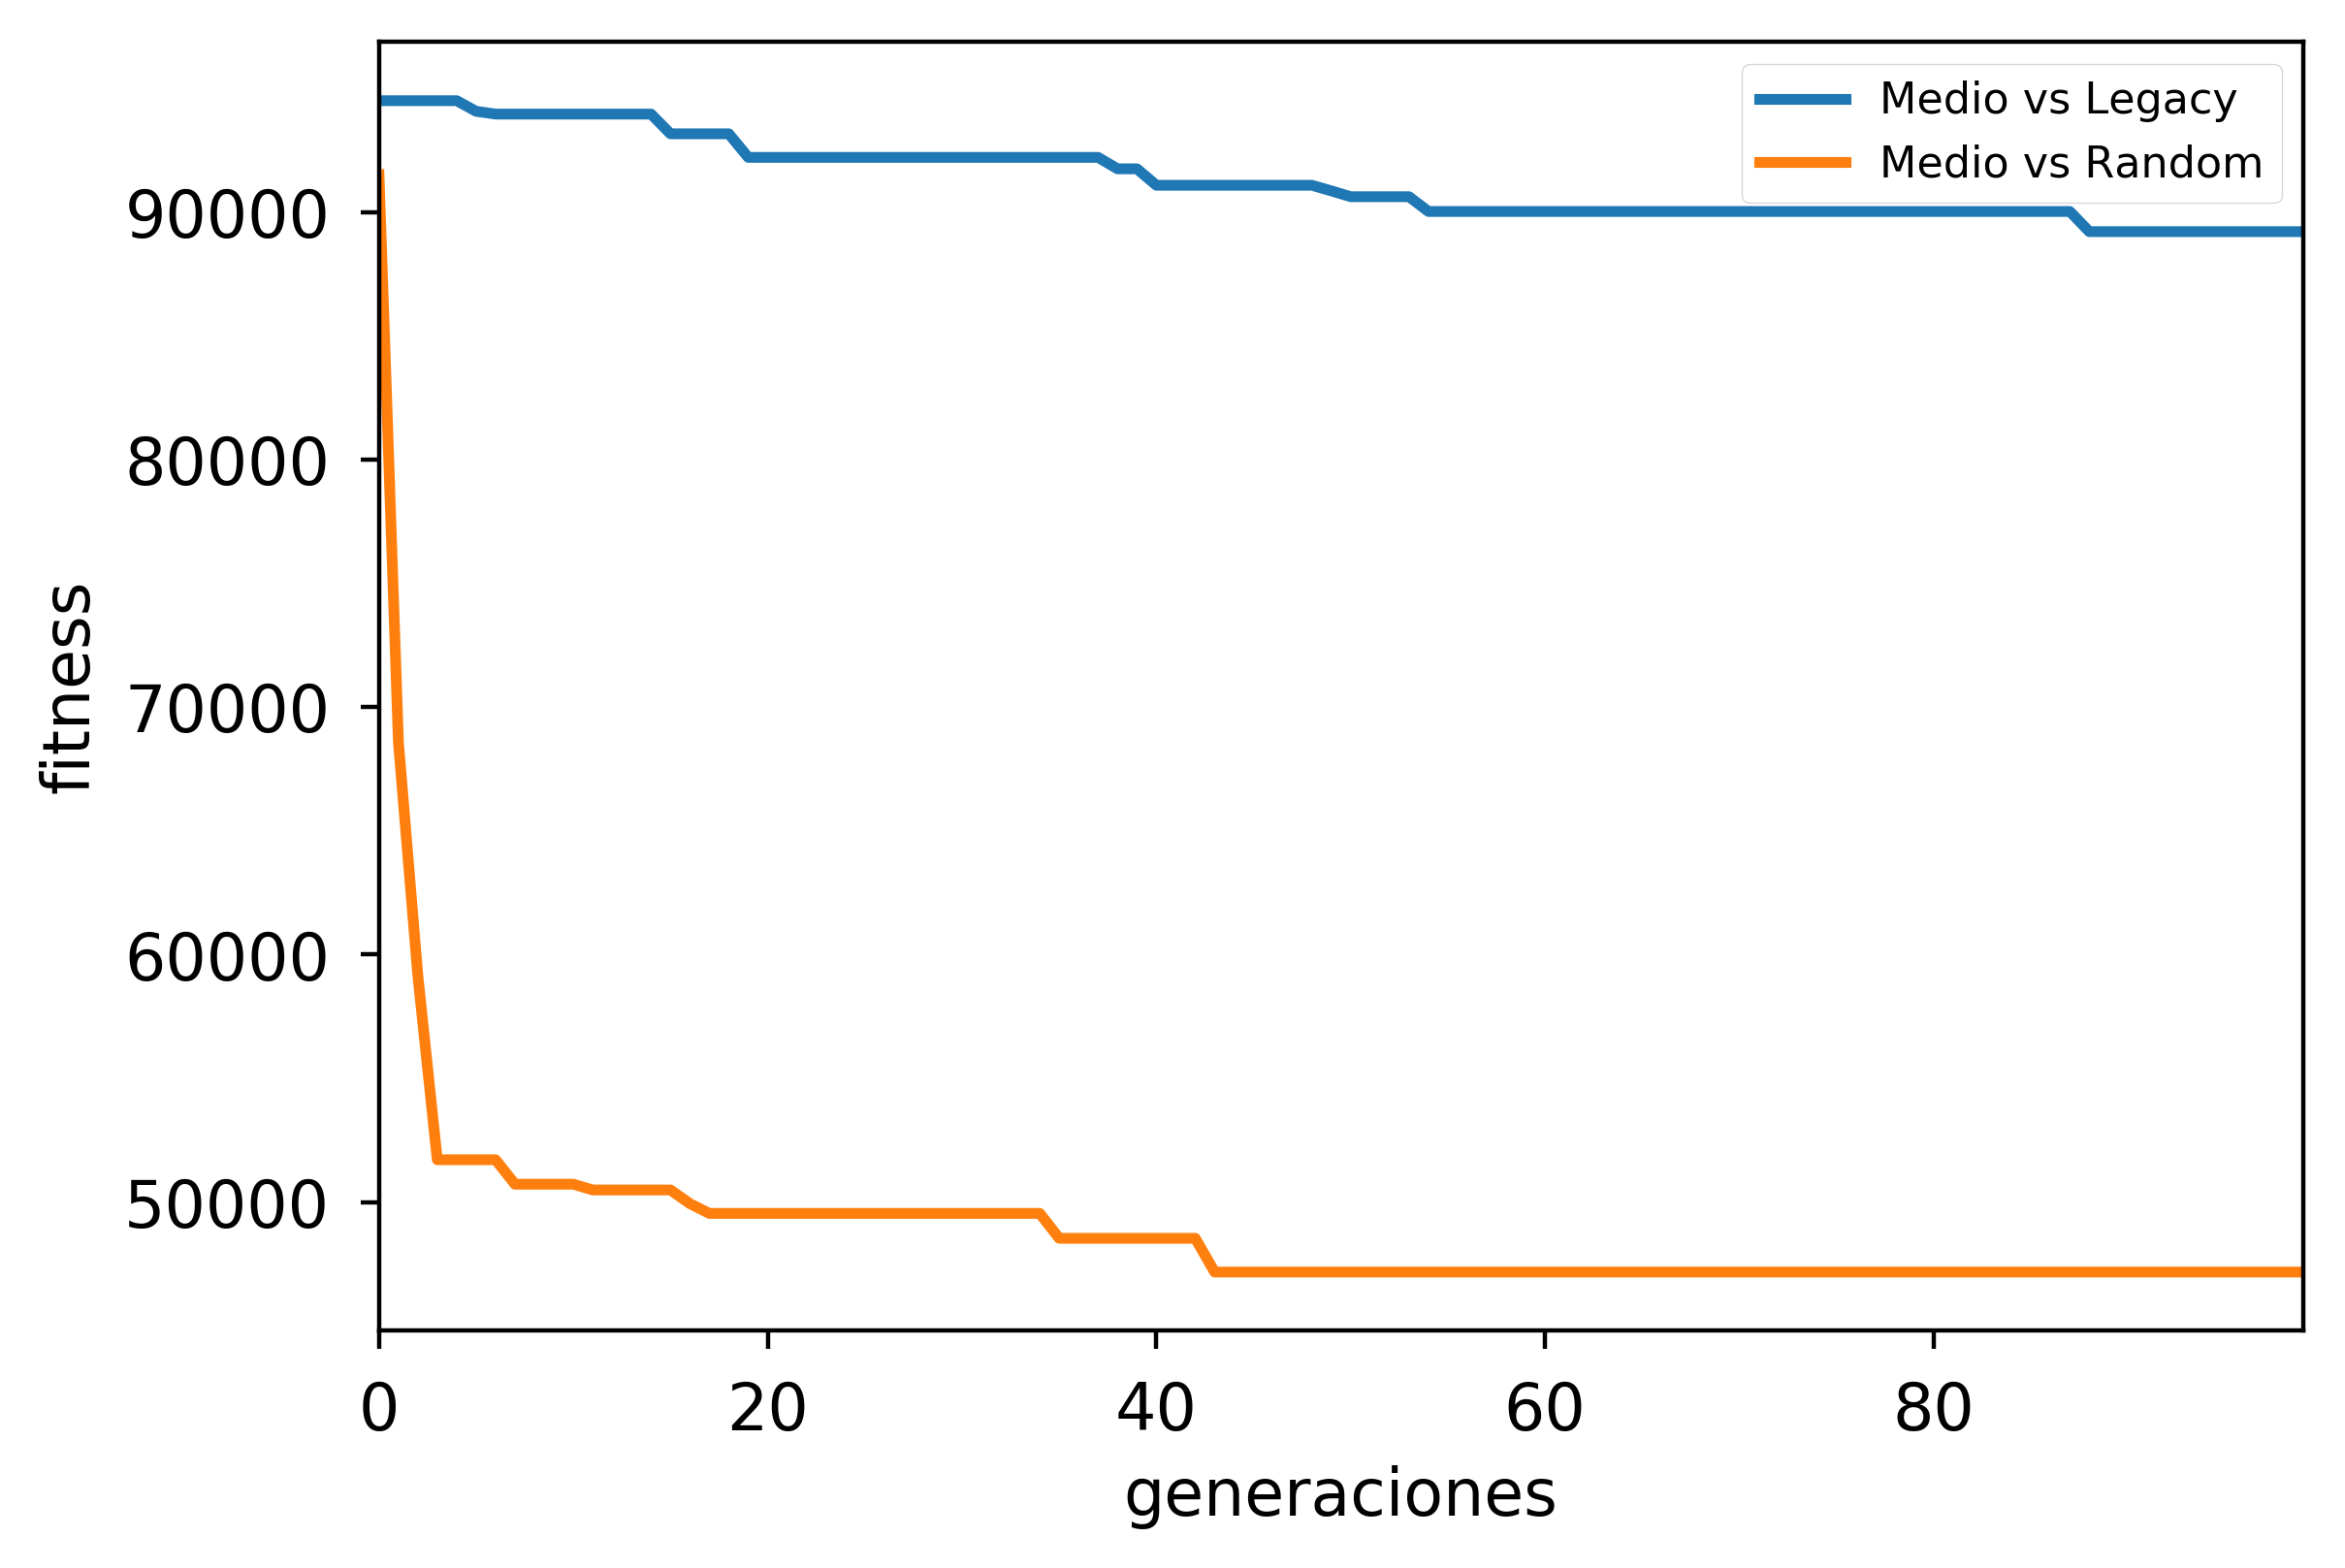
\includegraphics[width=0.8\textwidth]{grafica/medium_level}
\caption{Gráfica que muestra las primeras 100 generaciones de dos ejecuciones distintas contra los controladores de fantasmas Random y Legacy usando la gramática de medio nivel. Función fitness: 1000000 - puntos obtenidos.}
\end{figure}

Las conclusiones obtenidas son:
\begin{itemize}
\item La velocidad de ejecución del algoritmo evolutivo ha sido significativamente más rápida que la de bajo nivel, de forma que la ejecución se realiza en apenas unos minutos.

\item Los resultados obtenidos en puntos son bastante superiores a los obtenidos con la gramática de bajo nivel.

\item El código generado por el mejor individuo (fenotipo) es muy corto, generalmente consiste de un solo \textit{if-else} que contiene cada uno una única función.

\item Creemos que la longitud del código está directamente relacionada al comportamiento que poseen los mejores individuos y que es obtenido de forma recurrente. Al principio y si no hay fantasmas cercanos el bot solo realiza movimientos neutros (continuar en la misma dirección), quedándose atascado en una esquina del mismo modo que lo hace el bot ``Camper'' de la gramática de nivel bajo. Pero si un fantasma se acerca lo suficiente el bot pasa a un modo agresivo dirigiéndose a la \textit{power pill} más cercana, comiéndosela y cazando a tantos fantasmas como puede. Este comportamiento lo repite con todas las \textit{power pills} hasta que se queda sin ellas, pasando a un estado de movimiento neutral y siendo eliminado por los fantasmas sin pasar nunca del primer nivel del juego. Este comportamiento es debido a una característica del juego que provoca una explosión en la puntuación al comer fantasmas seguidos. Esto se debe a que durante el tiempo que dura el efecto de una \textit{power pill} cada fantasma comido da una serie de puntos, este valor es duplicado si se come otro fantasma y el nuevo valor es a su vez duplicado si otro fantasma es consumido. Esto permite obtener una gran cantidad de puntos provocando que el fitness de ese individuo destaque
\end{itemize}

Como se puede apreciar, la gramática de bajo nivel siempre lleva a un comportamiento de bot ``Camper'' y la gramática de medio nivel a un comportamiento de bot ``Cazador''. Estos comportamientos vienen dados principalmente por los puntos que se obtienen al jugar, por lo que investigamos el uso de una gramática de alto nivel y comparamos los resultados obtenidos con la gramática de medio nivel. Así mismo estudiamos distintas funciones \textit{fitness} y comprobamos si con estas nuevas funciones conseguimos mejores comportamientos.

\begin{lstlisting}[caption={Mejor individuo producido usando la gramática de medio nivel para evolucionar contra Random Ghosts.}]
    if (getDistanceToClosestNonEdibleGhost > 10) {
        if (getDistanceToClosestNonEdibleGhost < 20) {
            getDirectionTowardsClosestPowerPill 
        }
        else {
            getDirectionTowardsClosestPill
        }
    }
    else {
        getDirectionAwayFromClosestNonEdibleGhost
    }
\end{lstlisting}

\begin{lstlisting}[caption={Mejor individuo producido usando la gramática de medio nivel para evolucionar contra Legacy Ghosts.}]
    if (getDistanceToClosestNonEdibleGhost >= 5) {
        getDirectionTowardsClosestPill
    } else {
        getDirectionAwayFromClosestNonEdibleGhost
    }
\end{lstlisting}

\subsection{Gramática de alto nivel}
Tras los resultados obtenidos con las gramáticas anteriores, decidimos estudiar hasta qué punto sería posible mejorarlos mediante el empleo de una gramática de alto nivel, empleando  un número reducido de funciones de alto nivel, proporcionándole de esta forma conocimiento experto.

\subsubsection{Nuevas funciones de alto nivel}

\paragraph{escapeHL}
Genera un movimiento de huida hacia la \textit{power pill} mas cercana si puede alcanzarla antes que el fantasma más cercano. Si no llega a tiempo o bien no quedan \textit{power pill}s, genera un movimiento de huida del fantasma más cercano en la dirección que más le aleje de él.

\paragraph{attackHL}
Genera un movimiento hacia el fantasma más comible cercano siempre que este pueda ser alcanzado por otro fantasma no comible antes. Si no hay fantasmas comibles, genera un movimiento igual a la última dirección en la que se movió.

\paragraph{seekFoodHL}
Genera un movimiento hacia la \textit{pill} más cercana (o si no quedan \textit{pills}, la \textit{power pill} más cercana) siempre y cuando sea alcanzable por Pac-Man antes que por un fantasma. Si no llega a tiempo, mueve en la última dirección en la que lo hizo el turno anterior.

\subsubsection{Notación BNF}
\begin{lstlisting}[caption={Gramática de alto nivel.}]
<grammar> ::= <selection-statement>

<selection-statement> ::= if( <condition> ){ <statement> }
                          else{ <statement> }
                        | if( <condition> ){ <statement> }

<statement> ::= <terminal-func>
              | <selection-statement>

<terminal-func> ::= escapeHL
                  | attackHL
                  | seekFoodHL

<condition> ::= <number-func> <number-operator> <number>

<number-func> ::= getDistanceToClosestNonEdibleGhost
                | getDistanceToClosestEdibleGhost

<number-operator> ::= ==
                    | !=
                    | <
                    | >
                    | <=
                    | >=

<number> ::=  5 | 10 | 15 | 20 | 25 | 30
           | 40 | 50 | 60 | 75 | 80 | 90
\end{lstlisting}

\subsubsection{Resultados}
Debido al conocimiento experto que poseen las funciones, la gramática utilizada solo contiene como operadores de acción las tres funciones de alto nivel comentadas, dos operadores de obtención de información del tablero  (\texttt{getDistanceToClosestNonEdibleGhost} y \texttt{getDistanceToClosestEdibleGhost}) debido a que recurrentemente han sido las más utilizadas, el comportamiento de los mejores bots obtenidos con las gramáticas anteriores se basan únicamente en ellas para la toma de decisiones.
\begin{figure}[H]
\centering
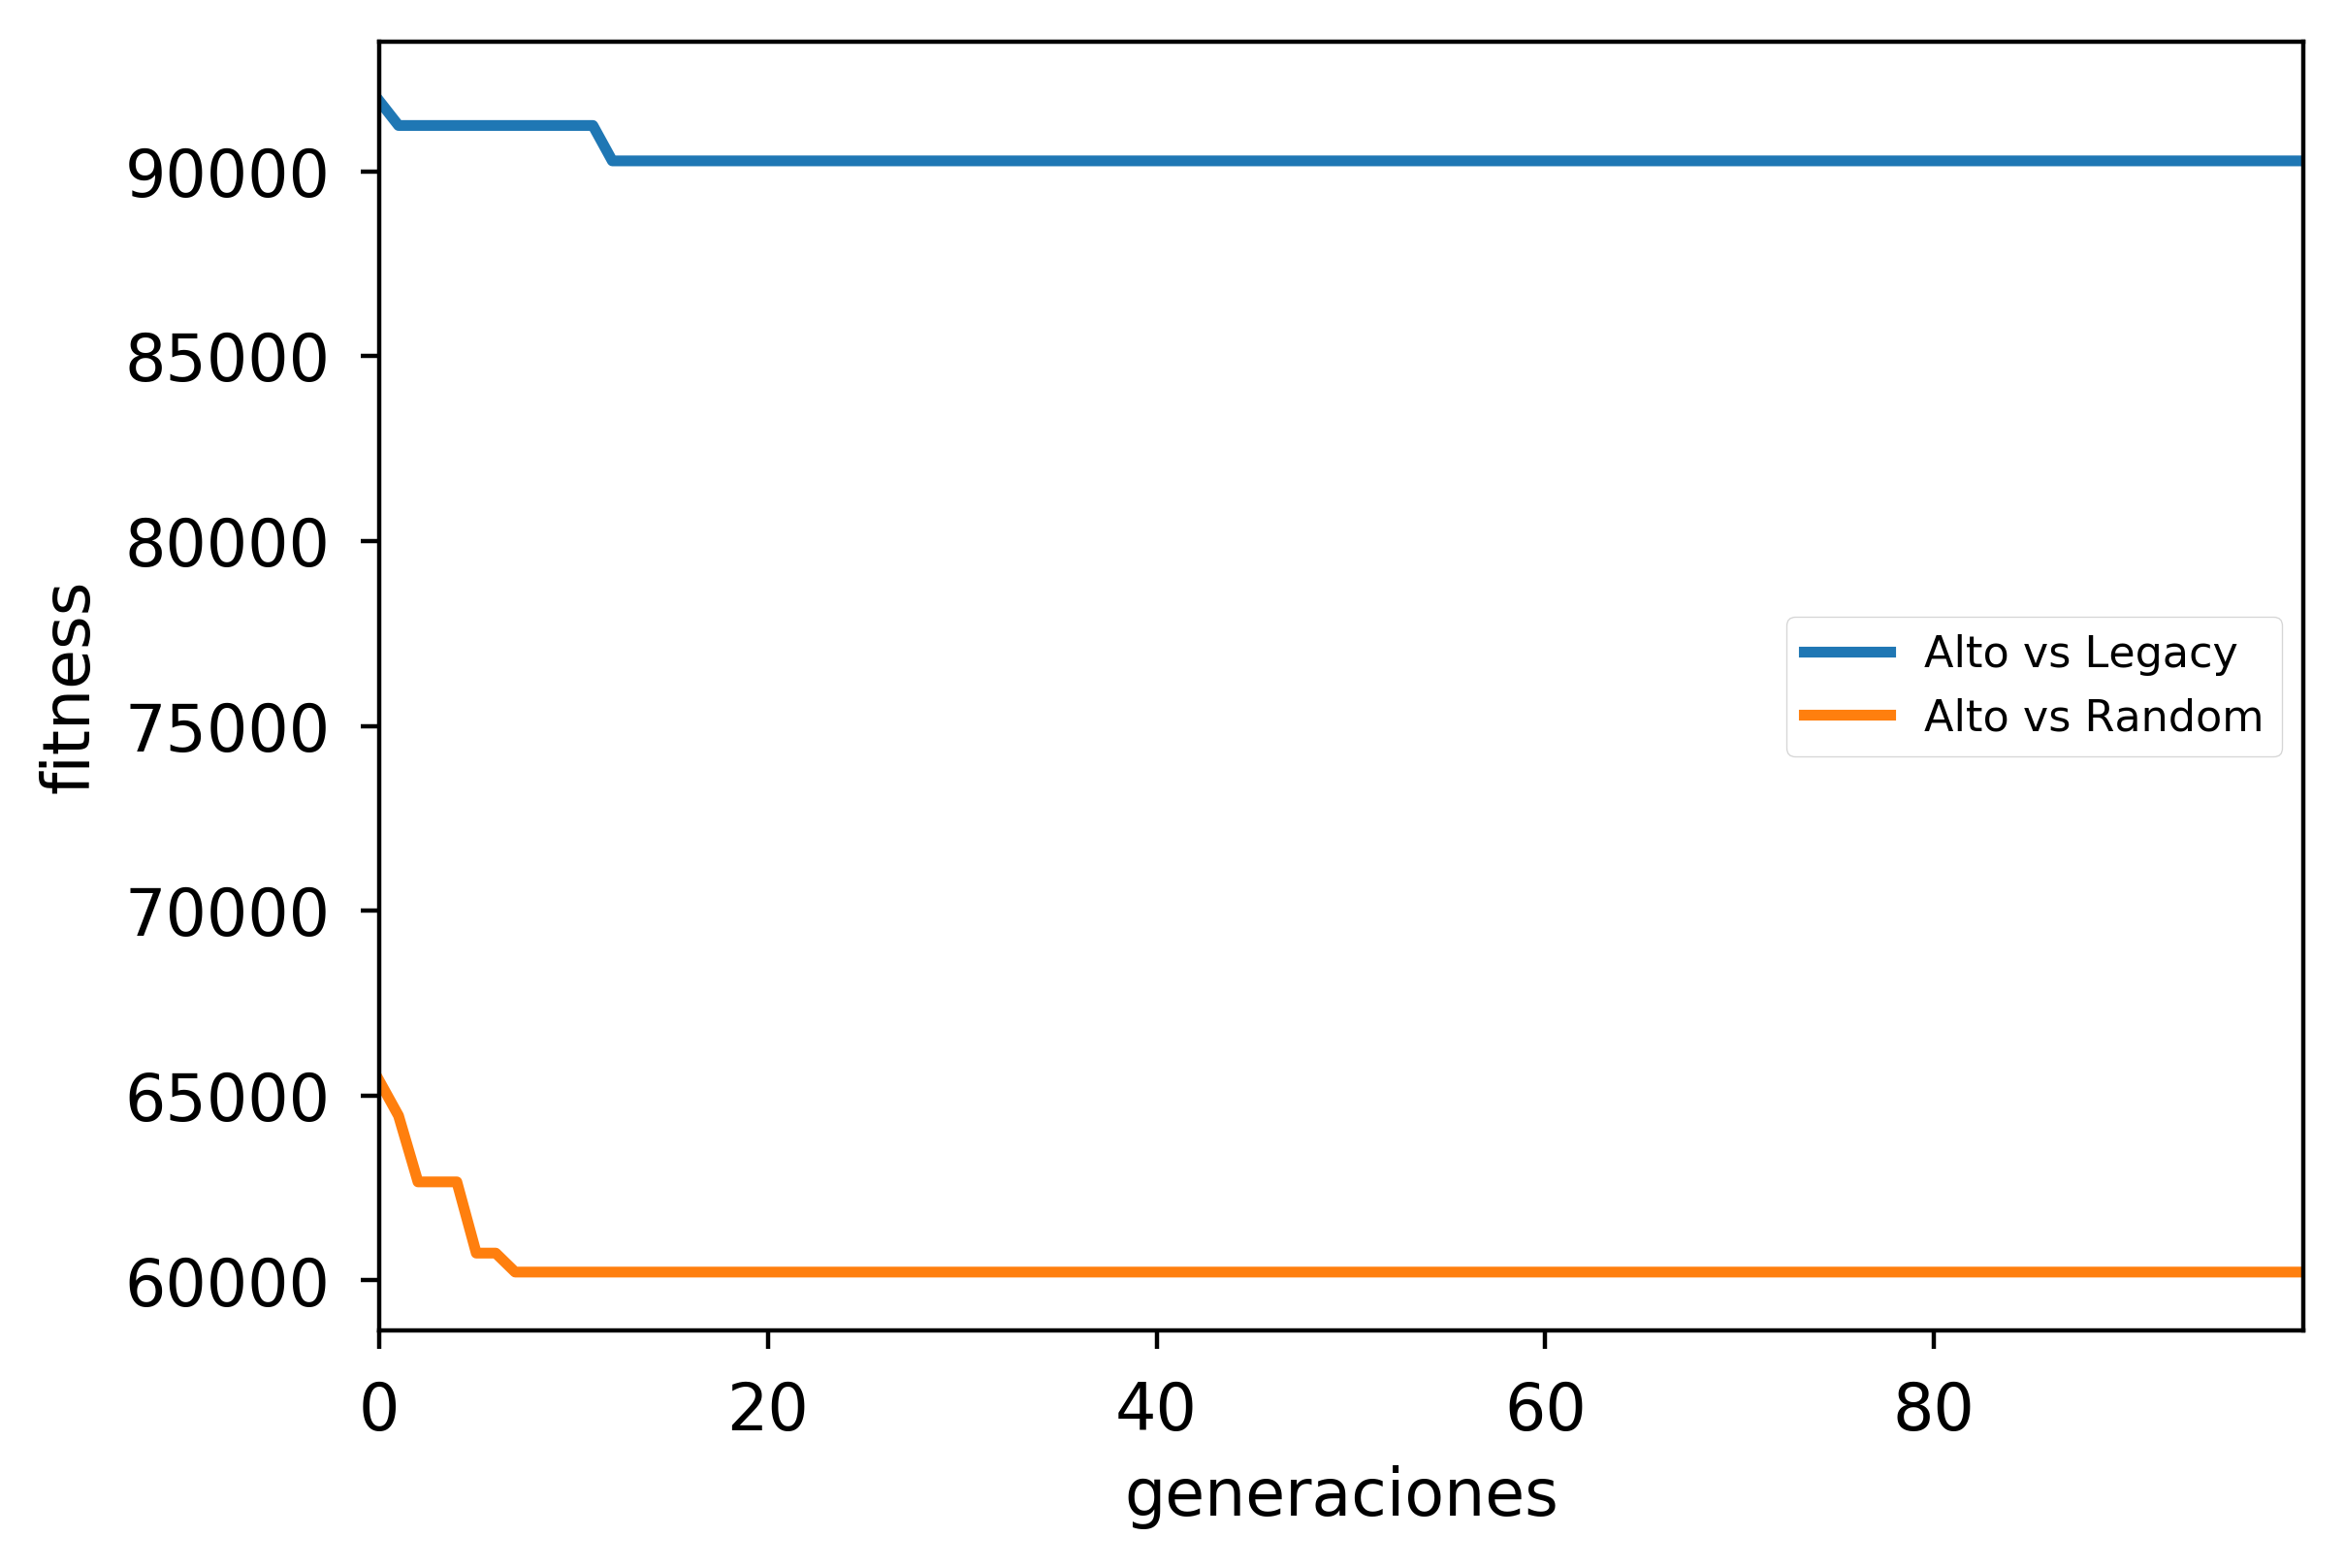
\includegraphics[width=0.8\textwidth]{grafica/high_level}
\caption{Gráfica que muestra las primeras 100 generaciones de dos ejecuciones distintas contra los controladores de fantasmas Random y Legacy usando la gramática de alto nivel. Función \textit{fitness}: $1000000 - puntos obtenidos$.}
\end{figure}

Las conclusiones obtenidas al evolucionar el bot usando esta gramática fueron:
\begin{itemize}
\item La velocidad de ejecución del algoritmo es aún más rápida que con la gramática de medio nivel, de forma que la ejecución se realiza en apenas unos segundos.

\item El código generado habitualmente se parece mucho al obtenido mediante la gramática de medio nivel: Un \textit{if-else} con una inecuación numérica que generalmente tiene en cuenta el fantasma más cercano. La más notable diferencia es que las acciones de medio nivel como \texttt{getDirectionAwayFromClosestNonEdibleGhost}, se ven sustituidas por su correspondiente directa de alto nivel, como \texttt{escapeHL}.
\begin{lstlisting}[caption={Código del mejor individuo obtenido en una población evolucionada con la gramática de medio nivel.}]
    if (getDistanceToClosestNonEdibleGhost >= 5) {
        getDirectionTowardsClosestPill
    } else {
        getDirectionAwayFromClosestNonEdibleGhost
    }
\end{lstlisting}

\begin{lstlisting}[caption={Código del mejor individuo obtenido en una población evolucionada con la gramática de alto nivel.}]
    if (getDistanceToClosestNonEdibleGhost <= 5) {
        escapeHL
    } else {
        seekFoodHL
    }
\end{lstlisting}

\item Obtiene buenos resultados muy rápidamente comparada con la gramática de medio nivel (Figura~\ref{grafica:comparacion-todas}). Esto se debe probablemente al reducido espacio de búsqueda de soluciones al ser una gramática tan compacta. Sin embargo y como se analizó en nuestro artículo (Apartado~\ref{cap:paper}),  la evolución utilizando la gramática de alto nivel se estanca en un óptimo local y es superada por la de medio nivel que obtiene mejores resultados, como se puede apreciar en la Figura~\ref{grafica:comparacion-todas}. La de medio nivel consigue algunos puntos más en promedio con 100 generaciones.
\end{itemize}

Todo esto nos indica que para tareas en las que es importante obtener buenos resultados de forma rápida, conviene favorecer gramáticas de alto nivel, mientras que si buscamos los mejores resultados posibles a cambio de un tiempo de evolución largo, conviene usar gramáticas de medio nivel.

\begin{lstlisting}[caption={Ejemplo de bot producido al evolucionar usando la gramática de alto nivel (mismo resultado entrenando tanto contra Random Ghosts como Legacy Ghosts).}]
    if (getDistanceToClosestNonEdibleGhost <= 5) {
        escapeHL
    } else {
        seekFoodHL
    }
\end{lstlisting}

\subsection{Comparativa gráfica de niveles}
\begin{figure}[H]
\centering
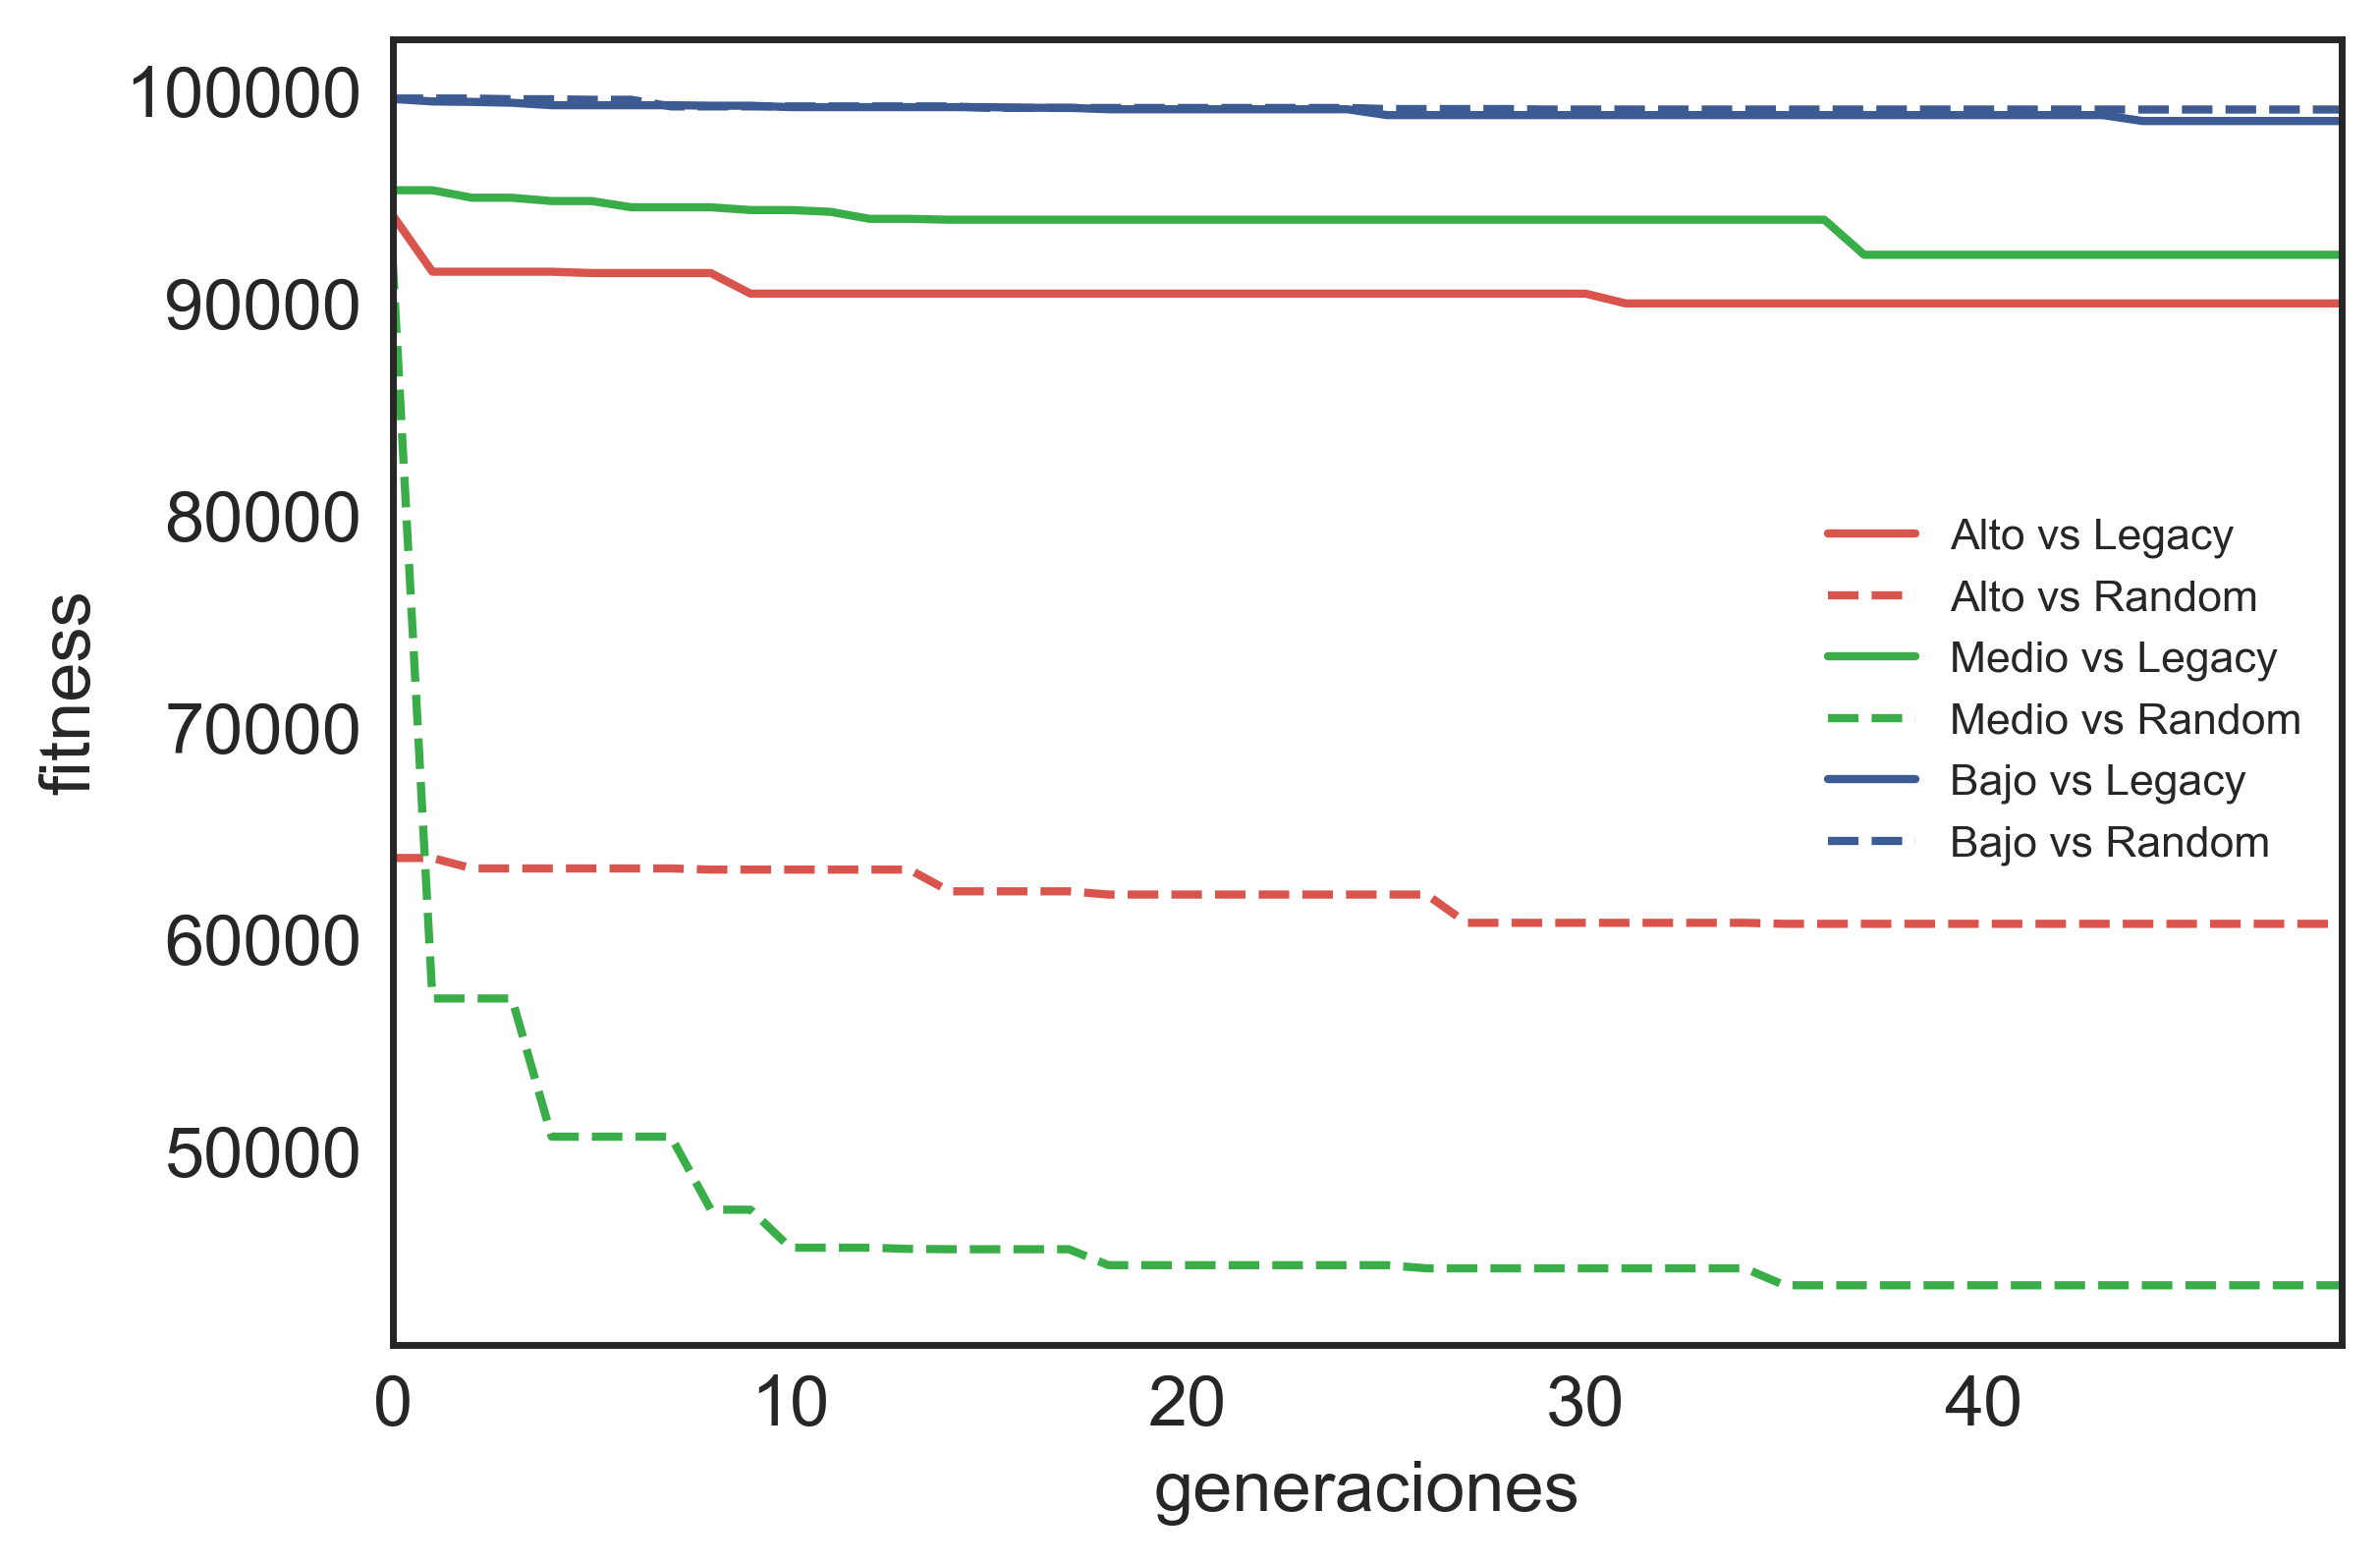
\includegraphics[width=0.8\textwidth]{grafica/all_fitnesses}
\label{grafica:comparacion-todas}
\caption{Gráfica de comparación de la evolución de una misma población usando las gramáticas de bajo, medio y alto nivel para dos controladores de fantasmas distintos (menos es mejor).}
\end{figure}

\chapter{Estudios, optimizaciones y mejoras} \label{cap:analisis}
Llegados a este punto nos planteamos realizar varios estudios relativos al rendimiento del algoritmo evolutivo, basadas en inquietudes fundadas en numerosos artículos científicos, para verificar que no se estaba produciendo ninguna inconsistencia dentro del entrenamiento de dicho algoritmo evolutivo. Además, también realizamos una serie de optimizaciones sobre funciones ya existentes en JECO, con el fin de reducir lo máximo posible el tiempo de ejecución y retocar algunas opciones por defecto del framework evolutivo para mejorar los resultados.

\section{Estudio de la presión selectiva}
Una de los factores que consideramos de importancia dentro de nuestro algoritmo evolutivo es la conservación de diversidad dentro de nuestra población y tratar de evitar el estancamiento en óptimos locales, la convergencia prematura y la evolución en avalancha producidas por la falta de ésta diversidad. Para ello hemos decidido evaluar cuál es la presión selectiva durante la ejecución, siendo esta la frecuencia con que es seleccionado el mejor individuo frente al resto. Esto se calcula en problemas de maximización mediante la siguiente fórmula
\begin{equation*}
\textrm{Presión selectiva} = \frac{\textrm{fitness mejor}}{\textrm{fitness promedio}}
\end{equation*}
En nuestro caso, al ser el nuestro un problema de minimización ($100000 - score$) empleamos:
\begin{equation*}
\textrm{Presión selectiva} = \frac{\textrm{fitness promedio}}{\textrm{fitness mejor}}
\end{equation*}

Habitualmente se recomienda emplear una presión selectiva en torno a $1.5$ \cite{whitley1989genitor}, mientras que nosotros a partir de mediciones hemos comprobado que empleamos una de aproximadamente $1.35$. Además, cada vez que se produce una mejora del mejor \textit{fitness}  se produce un aumento proporcional en la presión selectiva, volviéndose a equilibrar al adaptarse el \textit{fitness} promedio a esta mejora. No obstante, dicho aumento de la presión selectiva es despreciable.
 
Concluimos que tenemos una presión selectiva adecuada y por tanto no requerimos la implementación de ningún sistema de escalado del \textit{fitness} de los individuos para mantener una conservación de diversidad.
\begin{figure}[H]
\centering
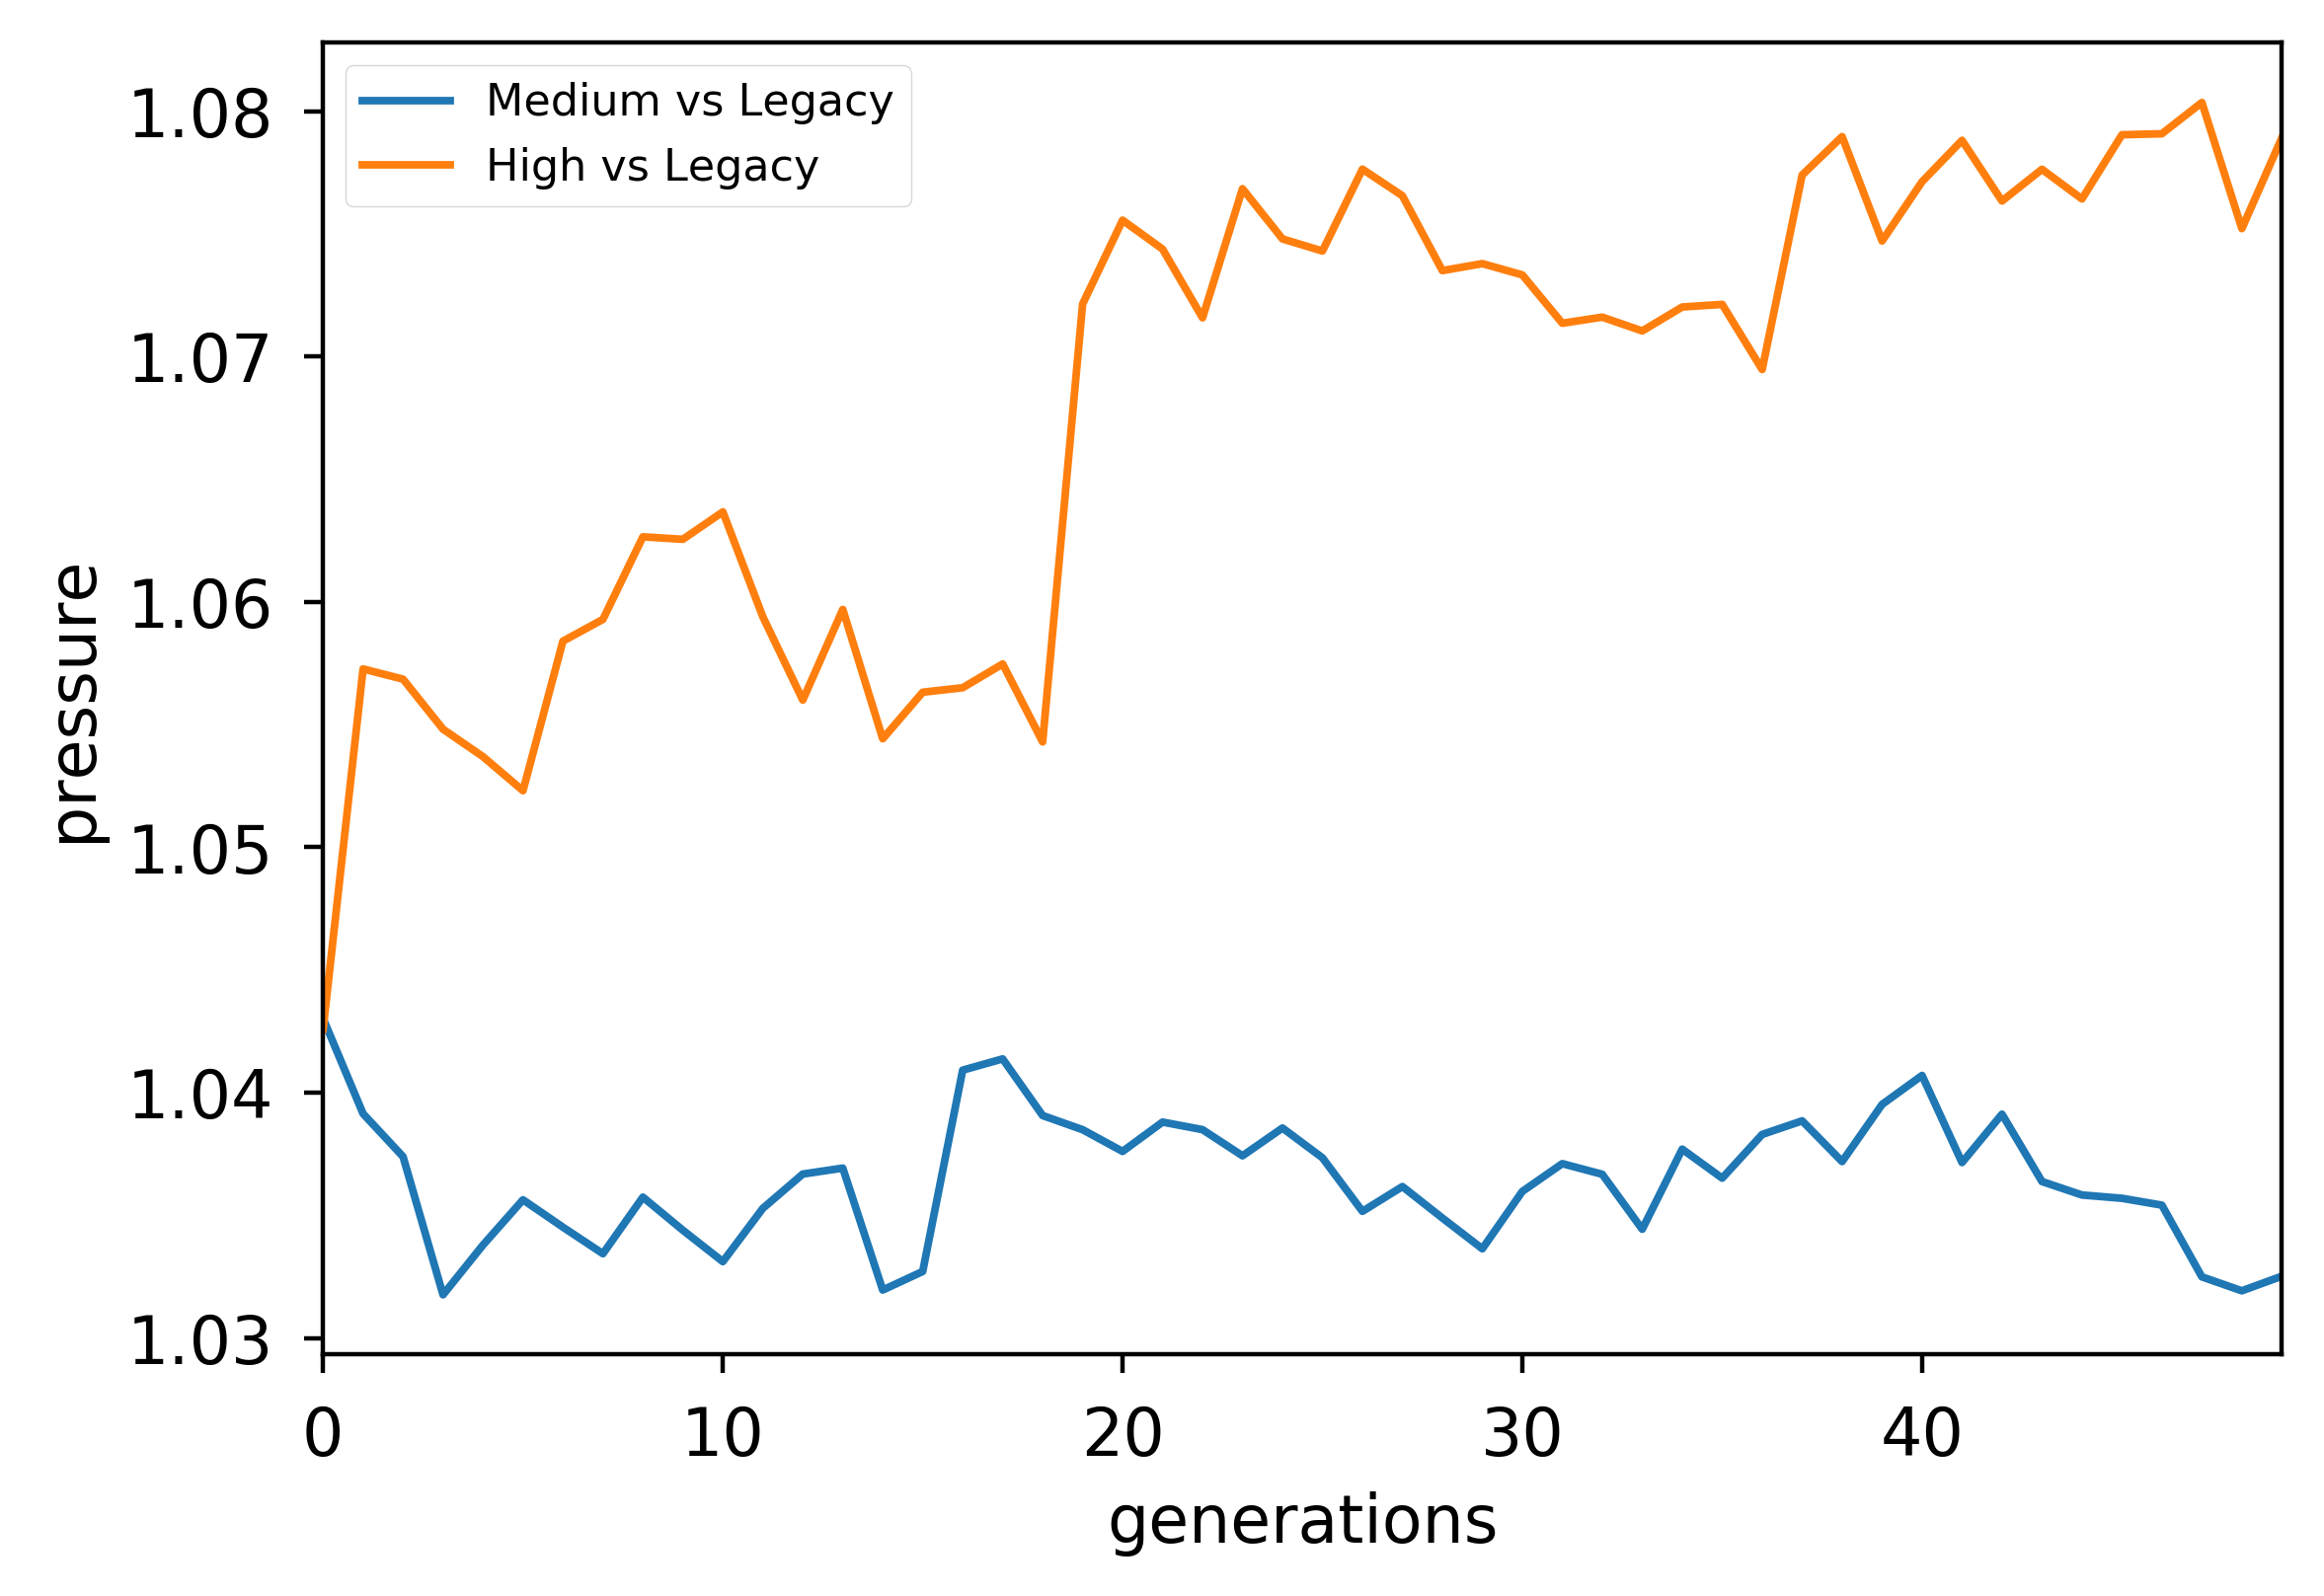
\includegraphics[width=0.8\textwidth]{grafica/presion-selectiva-detalle}
\caption{Vista en detalle  de la presión selectiva.}
\end{figure}

\begin{figure}[H]
\centering
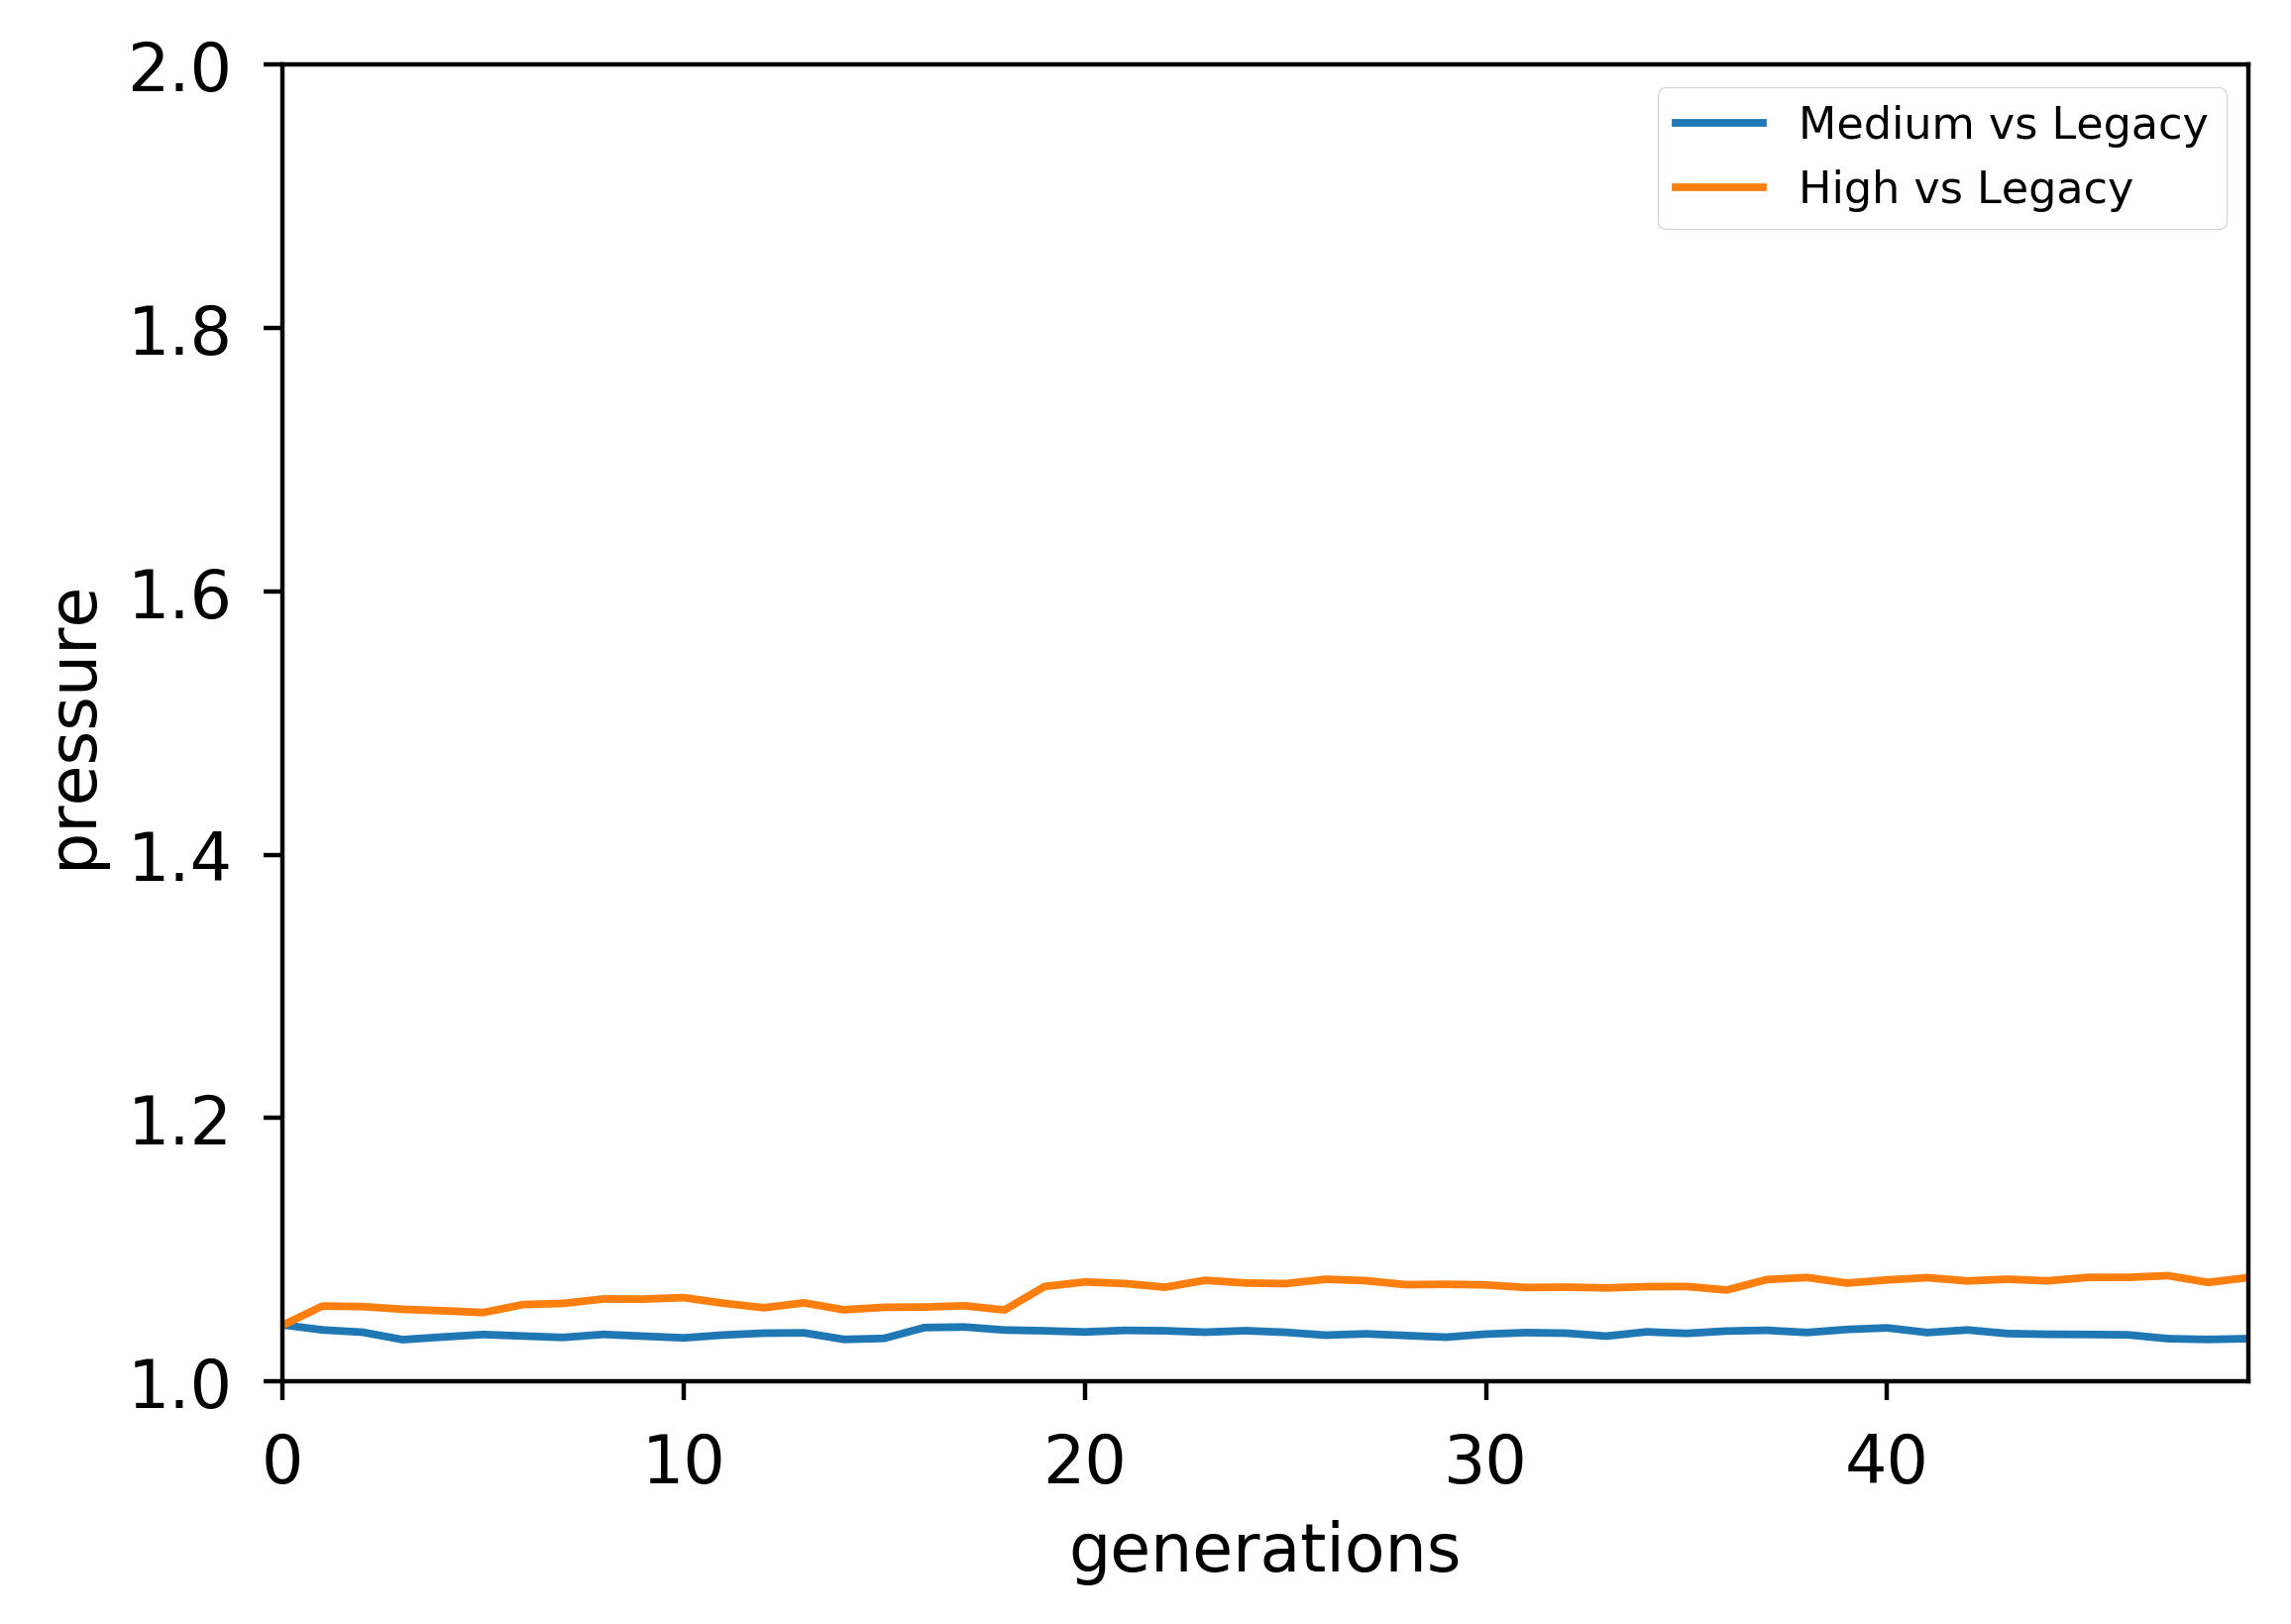
\includegraphics[width=0.8\textwidth]{grafica/presion-selectiva-general}
\caption{Vista global de la presión selectiva.}
\end{figure}

Además, tras un estudio en profundidad de nuestros operadores de selección hemos comprobado que todos (Torneo Binario, Torneo Binario NSGA y Torneo n-ario) emplean alguna modificación del operador de torneo, siendo este independiente al valor de la presión selectiva. Esto es así porque estos operadores no tienen en cuenta comparaciones entre fitness relativos (por ejemplo seleccionar proporcionalmente más veces los individuos con mejor fitness) sino comparaciones directas (seleccionar el individuo con mejor fitness entre varios elegidos de forma completamente aleatoria).

\section{Cruce LHS}
Antes de proceder con el estudio de nuevas funciones de \textit{fitness} decidimos comprobar si la razón por la que se producían programas tan cortos en las gramáticas de medio y alto nivel era por culpa del operador de cruce utilizado.

El operador de cruce monopunto usado en Gramáticas Evolutivas tiene el problema de generar mucho ruido en la población porque al cruzar los dos genotipos el nuevo hijo no suele guardar ninguna relación con los padres dada la forma en que se genera el fenotipo. Visto de otra forma, el cruce no copia un trozo de código de un individuo en el código del otro individuo, sino que lo altera desestructuradamente.

Para resolver este problema se implementa el cruce LHS que intenta solventar este problema. El cruce LHS, al igual que el monopunto, elige un punto aleatorio del genotipo pero en vez de cruzar la parte del genotipo restante a partir de ese punto lo que hace es ver cuántos codones expanden el símbolo no terminal marcado por el punto de cruce. Una vez visto cuántos codones componen la derivación total de dicho símbolo estos se insertan en la posición del punto de corte en el otro individuo, donde también se ha realizado el mismo proceso.

Este nuevo cruce produce ligeramente mejores resultados y menos ruido en la población pero tampoco se aprecia una gran mejoría en general. Aún así se convierte en el principal cruce que utilizamos en adelante.

\section{Estudio de uso de codones}
Durante la implementación del cruce LHS hicimos un estudio del número de codones utilizado en cada individuo para generar el fenotipo. El estudio lo hacemos con individuos de 100 y 50 codones permitiendo hacer \textit{wrapping}\footnote{El Wrapping se produce cuando se han procesado todos los codones del genotipo y aún no se ha llegado a procesar todos los símbolos no terminales dejando el fenotipo incompleto por lo que se sigue expandiendo los símbolos sin procesar usando nuevamente los codones del principio del genotipo.} 3 veces.  Los resultados obtenidos son los siguientes:
\begin{figure}[H]
\centering
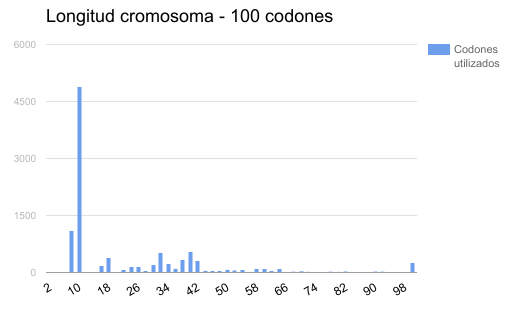
\includegraphics[width=0.8\textwidth]{grafica/codones-100}
\caption{Distribución del número real de codones utilizados. Longitud máxima 100 codones.}
\end{figure}

\begin{table}[H]
\centering
\begin{tabular}{|c|c|c|c|c|}
\hline
\textbf{Media} & \textbf{Wrappings} & \textbf{Moda} & \textbf{Mediana} & \textbf{Desviación  est.} \\ \hline
23.9           & 331                & 10            & 10               & 21.7                      \\ \hline
\end{tabular}
\caption{Estadísticas con longitud del cromosoma = 100.}
\end{table}

\begin{figure}[H]
\centering
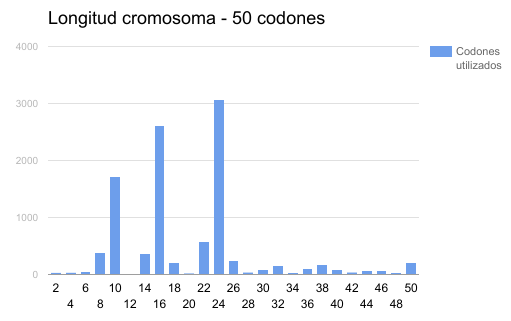
\includegraphics[width=0.8\textwidth]{grafica/codones-50}
\caption{Distribución del número real de codones utilizados. Longitud máxima 50 codones.}
\end{figure}

\begin{table}[H]
\centering
\begin{tabular}{|c|c|c|c|c|}
\hline
\textbf{Media} & \textbf{Wrappings} & \textbf{Moda} & \textbf{Mediana} & \textbf{Desviación  est.} \\ \hline
20           & 375                & 24            & 18               & 9                      \\ \hline
\end{tabular}
\caption{Estadísticas con longitud del cromosoma = 50.}
\end{table}

Como se puede ver, cuando se usan longitudes de 100 codones los fenotipos se generan en su mayoría usando solo diez codones, lo que implica programas muy cortos y que la mayoría de las mutaciones y cruces sobre ellos no tienen efecto dado que se producen en el 90\% de los codones del genotipo que no se usan.

En cambio, con una longitud de 50 codones los individuos suelen generar individuos más largos, usando 25, 16 y 10 codones normalmente. Lo que sugiere que longitudes más pequeñas de cromosomas implican programas más largos a los que una mutación o un cruce los afecta en mayor medida y que pueden llegar a generar mejores resultados.

Para comprobar esto realizamos un banco de pruebas donde comprobar si es verdad que longitudes de cromosomas más cortas producen mejores resultados. Evolucionamos varias poblaciones idénticas pero variando en cada una la longitud de sus cromosomas, usando valores de 10 a 100 incrementados de diez en diez.

Los resultados obtenidos de este banco de pruebas no aportaron nada dado que los resultados y longitudes de fenotipos en las poblaciones con longitudes entre 40 y 100 eran prácticamente iguales, por lo que concluimos que la longitud del cromosoma no tiene mucha relación con los resultados obtenidos.

\section{Estudio de funciones fitness}
Como ya hemos visto, las gramáticas de bajo y medio nivel producen comportamientos demasiado específicos e incluso indeseados pero que consiguen muchos puntos. Hemos decidido probar nuevas funciones y ver el comportamiento obtenido por el bot. Para estas pruebas utilizaremos la última versión de la  gramática de nivel medio y con los mismos valores y operadores para los operadores de cruce, mutación, etc (Apartado~\ref{sec:params}).
\begin{itemize}
\item \textit{Puntuación \{1000000 - puntuación media\}}: Es la función de \textit{fitness} que se utiliza de forma genérica. Puntúa a los individuos por la puntuación media obtenida al evaluarlos, siendo los mejores individuos aquellos que obtengan mayor puntuación media.

Esta función se estanca siempre en un óptimo local produciendo el bot ``cazador'' el cual solo busca comerse el mayor número de fantasmas dado que esta acción produce una gran cantidad de puntos, pero una vez acabadas las \textit{power pill} realiza movimientos neutrales o come la \textit{pill} más cercana sin importarle la posición de los fantasmas, por lo que es eliminado por los fantasmas y no es habitual que complete el nivel uno.

\begin{lstlisting}[caption={Mejor individuo obtenido mediante esta función fitness.}]
    if( getDistanceToClosestEdibleGhost <= 20 ){ 
        getDirectionTowardsClosestPowerPill
    }
\end{lstlisting}

\item \textit{Pills \{1000 - media de pills consumidas\}}: \textit{Fitness} que tiene como objetivo comer el máximo número de \textit{pills} posibles, sin importar la puntuación obtenida ni el nivel, aunque este último está directamente relacionado con comer \textit{pills}. Al mejor individuo que suele producir le hemos denominado bot ``Glotón''.

Este bot se centra únicamente en comer \textit{pills} normales pero, si se siente amenazado por un fantasma cercano, se dirige hacia una \textit{power pill}, la consume y sigue comiendo \textit{pills} normales (pero no caza a los fantasmas). Cuando no dispone de más \textit{power pills} a las que dirigirse y un fantasma se acerca, este sigue comiendo \textit{pills} normales y es comido por los fantasmas. Este bot suele perder en el nivel dos o en el nivel uno cuando quedan pocas \textit{pills} por comer. El código producido es el antónimo del producido por el \textit{fitness} de \textit{Puntuación}.

\begin{lstlisting}[caption={Mejor individuo obtenido mediante esta función fitness.}]
    if( getDistanceToClosestNonEdibleGhost >= 25 ){ 
        getDirectionTowardsClosestPill
    }
    else{ 
        getDirectionTowardsClosestPowerPill
    }
\end{lstlisting}

\item \textit{Niveles \{10 - máximo nivel alcanzado\}}: El objetivo de este \textit{fitness} es pasarse el mayor número de niveles sin importar la puntuación, las \textit{pills} comidas, el tiempo utilizado, etc por lo que los mejores individuos son los que han llegado al nivel más avanzado. Este bot nos sorprendió dado que aprovecha el fallo del juego que provoca que no sea detectado por algunos controladores de fantasmas como \textit{Starter ghosts}, si se coloca en una cierta posición del laberinto.

Este ``exploit'' lo conocíamos pero nunca se había producido en el nivel tres, sin embargo este bot consigue realizarlo en todos los niveles llegando a superar\footnote{La versión actual del juego soporta un número ilimitado de niveles pero dispones de un tiempo máximo de juego (24000 \textit{ticks}). El juego es detenido si se consume el tiempo total, independientemente del nivel en el que te encuentres. Dado que la versión actual del juego hace que se avance de nivel automáticamente al estar 4000 \textit{ticks} en el mismo nivel el número máximo de niveles al que se puede llegar usando el fallo del juego (estancándose en una parte del laberinto sin moverse hasta que se avanza de nivel por tiempo) es de $24000 / 4000 = 6$ niveles.} el juego. Se trata del bot ``Camper'' pero con un comportamiento mejorado. Nos dimos cuenta de que este comportamiento es alcanzable con las funciones \texttt{getDistanceToClosestJunction\{Up, Down, Right, Left\}}. Si eliminamos dichas funciones de la gramática de medio nivel entonces se produce un bot ``Camper'' que no supera el nivel cuatro.
\end{itemize}

Observamos que el bot se especializa dependiendo del objetivo de la función \textit{fitness} como es de esperar. No obstante contra controladores de fantasmas especialmente bien diseñados como \textit{Legacy} la diversidad de comportamientos decrece, ya que en Pac-Man la mayoría de objetivos están relacionados (por ejemplo, para pasarse niveles Pac-Man ha de comerse todas las \textit{pills} si le es imposible ``atascar'' a los fantasmas y ganar el nivel por agotar el tiempo).

En cualquier caso decidimos explorar una estrategia multiobjetivo con la intención de conseguir un comportamiento acorde a lo que se debería esperar de un jugador \textit{amateur}, avanzar el máximo número de niveles consiguiendo la mayor cantidad posible de puntos, comportamiento que no conseguimos usando una función \textit{fitness} con un único objetivo en consideración contra todos los tipos de fantasmas.

\section{Optimización Multiobjetivo}
Para intentar solventar el problema de especialización que se está produciendo contra algunos tipos de fantasmas decidimos implementar una estrategia multiobjetivo en el algoritmo.

Existen varios métodos de implementación de estrategias multiobjetivo y por la primera que nos decantamos fue una estrategia mediante funciones agregativas. Decidimos usar esta estrategia en primer lugar porque no altera el algoritmo de gramáticas evolutivas que estamos usando actualmente. Consiste en la implementación de una función \textit{fitness} (como hasta ahora) pero que consta de una combinación lineal de funciones o parámetros que cada una determina la valía de un individuo en un determinado aspecto.

\subsection{Funciones Agregativas}
La primera función agregativa mediante este método fue la unión de las anteriores funciones fitness de comer el máximo número de pills y alcanzar el mayor nivel. La unión directa de las funciones como una combinación lineal del estilo
\begin{equation*}
f = \textrm{nº de pills} + \textrm{nivel máximo alcanzado}
\end{equation*}
no es posible por la diferencia de escala de los objetivos (el número de \textit{pill} comidas va a ser siempre más grande que el nivel máximo alcanzado por lo que ese objetivo no tiene impacto visible en el \textit{fitness} del individuo) por lo que el uso de unos pesos $w_i$ serán necesarios para que ambas funciones tengan la misma importancia en la combinación lineal.

Dada la función
\begin{equation*}
f = w_0 * \textrm{nº de pills} + w_1 * \textrm{nivel máximo alcanzado}
\end{equation*}
tuvimos que experimentar varias versiones con distintos valores de los pesos wihasta conseguir un balance adecuado. La versión final de la función fue
\begin{equation*}
f = \textrm{nº de pills} + 10 * \textrm{nivel máximo alcanzado}
\end{equation*}
donde $w_0 = 0$ y $w_1 = 10$.

Los resultados no fueron los esperados y normalmente se obtenía un comportamiento de bot ``Glotón'' en los mejores casos pero se vio un incremento en la longitud media de los programas (fenotipo) evolucionados.

El mismo proceso se realizó con la unión de las funciones \textit{fitness} de conseguir puntos y avanzar de niveles
\begin{equation*}
f = 0.1 * \textrm{nº de puntos obtenidos} + \textrm{nivel máximo alcanzado}
\end{equation*}
donde $w_0 = 0.1$ y $w_1 = 1$ pero se obtuvo un bot ``Camper'' pero con un código menos eficiente y llegando hasta el cuarto nivel de media.

\begin{lstlisting}[caption={Código del bot Camper obtenido mediante funciones agregativas.}]
if( getDistanceToClosestJunctionLeft >= 60 ){ 
    getDirectionTowardsClosestPill
 }
 else{ 
    if( getDistanceToClosestEdibleGhostUp > 75 ){ 
        if( getClosestEdibleGhostDistanceToClosestJunctionLeft < 30 ){ 
            if( getDistanceToClosestNonEdibleGhost <= 50 ){ 
                getDirectionTowardsClosestEdibleGhost
             }
             else{ 
                getDirectionTowardsClosestEdibleGhost
             }
         }
         else{ 
            if( getDistanceToClosestNonEdibleGhost <= 10 ){ 
                if( getClosestEdibleGhostDistanceToClosestJunctionDown <= 5 ){ 
                    getDirectionAwayFromClosestNonEdibleGhost
                 }
                 else{ 
                    getDirectionTowardsClosestPowerPill
                 }
             }
 
         }
     }
     else{ 
        getDirectionTowardsClosestPill
     }
 }
\end{lstlisting}

Nuevamente no obtenemos los resultados esperados y el proceso de creación de combinaciones lineales es experimental, poco preciso y tedioso, así que nos decidimos a realizar una implementación avanzada de la estrategia multiobjetivo mediante el uso del algoritmo NSGA-II el cual usa la definición de óptimo de Pareto y frente de Pareto en su algoritmo para determinar los mejores individuos en los objetivos a optimizar.

\subsection{NSGA-II}
JECO disponía de una implementación del algoritmo NSGA-II que nos sirvió como base para desarrollar la implementación de la estrategia multiobjetivo mediante NSGA-II. Los cambios realizados en JECO a nivel de código se explicarán en el apartado~\ref{sec:multi}).
 
Hemos desarrollado una serie de funciones fitness por cada objetivo que deseemos optimizar. Hemos intentado representar los objetivos típicos que un jugador humano amateur intenta conseguir.

\paragraph{Naive fitness}
Puntuación directa obtenida en juego, en la que se tienen en cuenta \textit{pills}, \textit{power pills} y fantasmas comidos. Cuantos más puntos mejor \textit{fitness} obtenido (minimización).
\begin{equation*}
f = 1000000 - \textrm{puntuación media}
\end{equation*}

\paragraph{Ghosts eaten}
Número de fantasmas comidos. Cuantos más fantasmas consumidos mejor fitness tendrá el individuo.
\begin{equation*}
f = 1000 - \textrm{fantasmas comidos}
\end{equation*}

\paragraph{Levels completed}
Número de niveles completados. A mayor nivel alcanzado mejo fitness del individuo.
\begin{equation*}
f = 100 - \textrm{último nivel alcanzado}
\end{equation*}

\paragraph{Points without ghost multiplier}
La puntuación total obtenida pero sin emplear el multiplicador de puntos que utiliza Pac-Man al comer varios fantasmas seguidos.
\begin{equation*}
\begin{split}
f = 100000 - (\textrm{número de pills consumidas} * \textrm{puntos por pill consumida}) \\
+ (\textrm{número de power pills consumidas} * \textrm{puntos por power pill consumida}) \\
+ (\textrm{número de fantasmas consumidos * puntos por fantasma consumida})
\end{split}
\end{equation*}

\subsection{Resultados}
Desafortunadamente, la inclusión de multiobjetivo no parece marcar una diferencia notable. Si por ejemplo usamos los \textit{fitness} \textit{Naive} y \textit{Levels completed} no se obtienen mejores bots que los mismos \textit{fitness} por separado. Esto se debe a que los objetivos que se pueden crear para el juego dependen directa o indirectamente de la puntuación, por lo que no se crea diversidad de comportamiento en nuestros programas. Lo que nos lleva a pensar que funcionaría mucho mejor cuando los objetivos no están directamente relacionados.
 
Los resultados muestran que si forzamos el objetivo de alcanzar más niveles, los programas obtenidos alcanzan puntuaciones similares ya que Pac-Man avanza niveles comiendo todas las \textit{pills} del laberinto, y por tanto consiguiento puntuaciones más altas. Lo mismo pasa al contrario, si nos centramos en conseguir puntos, Pac-Man completará todos los niveles que le sea posible porque se centra en comerse todas las \textit{pills}.
 
De cualquier forma siempre tenemos una ventaja clara usando multiobjetivo; en vez de definir un comportamiento monolítico podemos crear un diseño más modular, más fácilmente, añadiendo subobjetivos adicionales a los ya escogidos. Como por ejemplo comer \textit{pills} y mantenerse lo más alejado posible de los fantasmas, lo que le hace sobrevivir más tiempo.

\section{Mutación neutral}
La Mutación Neutral es un operador específico para gramáticas evolutivas \cite{oesch2015neutral} que pretende proporcionar más diversidad a la población realizando una mutación que no afecta al fenotipo. Esto es posible en gramáticas evolutivas, ya que si modificamos un codón del fenotipo de un individuo sumándole un múltiplo del número de producciones de la regla que determinó esa parte del fenotipo, el fenotipo resultante es el mismo. Por ejemplo, si tenemos un símbolo no terminal expandible a través de cuatro reglas de producción a los codones mutados se les suma a su valor actual un múltiplo de cuatro (dado que hay cuatro reglas de producción) por lo que al generar el fenotipo y realizar el módulo al codón este devolverá el mismo número que antes de la mutación produciendo el mismo fenotipo.
Aunque se mantiene el mismo fenotipo del individuo, se gana una mayor diversidad, ya que en evaluaciones posteriores el genotipo de este individuo ha podido ser modificado a través del operador de cruce o un operador de mutación adicional que sí produzca cambios (como Mutación bit a bit) y este cambio en el codón ya no tiene por qué producir el mismo módulo y modificará el fenotipo.


\section{Multithread}
Al empezar a desarrollar el segundo bot también pudimos aprovechar otra funcionalidad de JECO que consiste en paralelizar la etapa más pesada del algoritmo (evaluación) en los distintos procesadores del ordenador.

Así, las etapas donde se ejecutan los operadores de selección, cruce y mutación se hacen en el mismo hilo de procesamiento, ya que estas etapas son más llevaderas, con algún operador ejecutándose por ejemplo un 10\% de las veces en la iteración. Y seguidamente cuando llegamos a la etapa de evaluación, podemos dividir la tarea entre tanto núcleos como haya disponibles para ejecutar el juego 1, 10, 20 o incluso más veces para paliar la aleatoriedad de los fantasmas, y eso para cada individuo de la población.

Gracias a esta técnica nos hemos podido permitir poblaciones más grandes y mayor número de generaciones en las evoluciones sin que los tiempos para completarlas sean desorbitados.


\section{Optimizaciones secundarias de JECO}
El framework JECO nos es de mucha ayuda, pero ha habido ciertos momentos en los que se necesitaban ciertos ajustes o carecía de ciertas funcionalidades que nos hacían falta, por lo que las hemos tenido que implementar a mano. Las más importantes son:

\subsection{Creación de las clases para cada función fitness}
Se implementó un patrón de diseño \textit{Command} para estructurar la creación de funciones de \textit{fitness}. Así todas las funciones, aunque dispares, tienen un punto común que funciona de acuerdo a lo esperado.

\subsection{Wrapper de funciones fitness para su uso en multiobjetivo} \label{sec:multi}
Gracias al patrón \textit{Command} para las clases de las funciones de fitness se pudo implementar una factoría de clases fitness y un envoltorio (\textit{FitnessWrapper}). A esta clase se le pasan las funciones creadas fácilmente desde \textit{ObjectiveFactory} cuando se quieren cambiar objetivos, incluso en tiempo de ejecución. Después, \textit{FitnessWrapper} es llamado cada vez que se evalúa el algoritmo en las sucesivas generaciones, justo después de ejecutar Pac-Man para pasarle las estadísticas de la partida.

\subsection{Modificación de la mutación}
La mutación por defecto en JECO se realiza únicamente sobre los individuos que son resultantes de un cruce. Mezclar cruce y mutación de esta manera no nos ha dado buenos resultados, y lo hemos sustituido por una aproximación más común en los Algoritmos Genéticos: Primero se aplica el operador de cruce a los elementos seleccionados de la población anterior, y después se aplica el operador de mutación a toda esa nueva población de elementos seleccionados e hijos generados por el operador de cruce. De esta manera garantizamos la independencia de operadores, ya que de lo contrario, tener una probabilidad de cruce muy baja implicaba que el operador de mutación se aplicase con una probabilidad distinta y solo a ciertos elementos.

\subsection{Modificación de la élite}
JECO utiliza un método particular a la hora de mantener la élite en la población. En cada generación y después de haber realizado la selección, cruce y mutación en los individuos pertinentes JECO unía la población antigua y la nueva población, constituida por los elementos seleccionados y los hijos creados a través de aplicar el operador de cruce, creando una unión de poblaciones ordenada de mejor a peor fitness. De este nuevo conjunto se extrae el número de individuos máximo que pueden haber en una población.

Este método no aporta diversidad a la población dado que se usa toda la población de la anterior generación (sin alterar) y la nueva población para generar la población final que será utilizada en la siguiente generación, haciendo que muchos individuos de la anterior generación se conserven en la nueva generación (y normalmente a lo largo de muchas generaciones más) conduciendo la búsqueda rápidamente a un óptimo local del cual es difícil de salir por falta de diversidad.

Optamos por deshacernos de esta implementación e implementamos un elitismo clásico, donde un subconjunto de los mejores individuos de la población antigua (determinado por un parámetro denominado porcentaje de elitismo) se incluyesen en la nueva generación sustituyendo un porcentaje idéntico de peores individuos en la nueva población, aportando mayor diversidad y permitiendo que la búsqueda no se estanque tan rápido en un óptimo local e incluso pudiendo salir de él.
\begin{figure}[H]
\centering
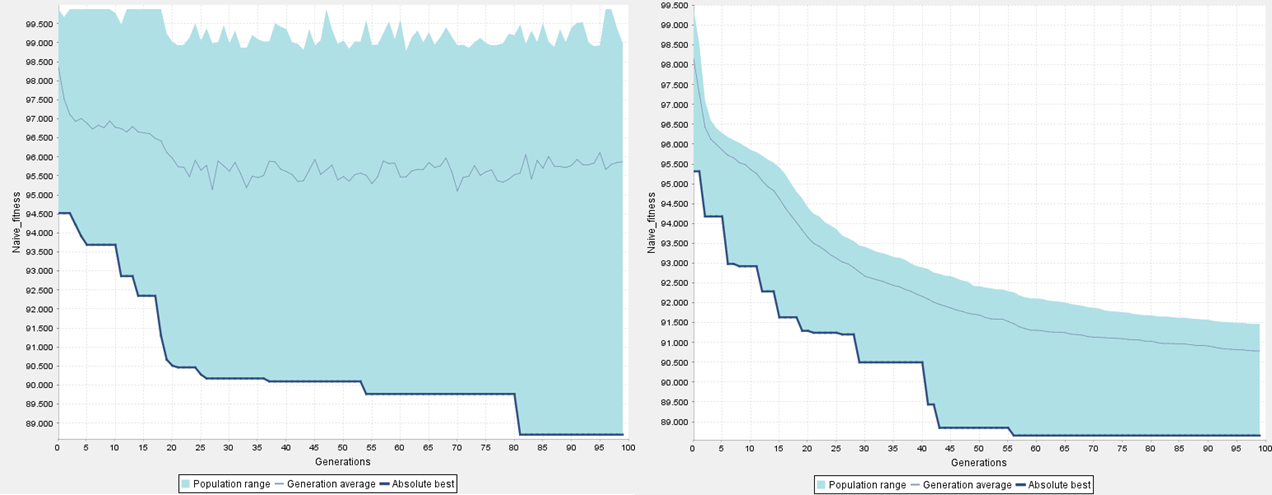
\includegraphics[width=\textwidth]{comparacion-elite}
\caption{A la izquierda gráfica de la evolución de la población con el nuevo método de elitismo. A la derecha gráfica usando el método de elitismo de JECO usado anteriormente. La línea gris muestra la media del fitness de la población.}
\end{figure}

\section{Batch Executor}
Debido que empleamos controladores de fantasmas no deterministas, necesitamos ejecutar varias partidas con un mismo controlador de Pac-Man para obtener resultados estadísticamente correctos de su rendimiento. Puesto que aumentar el número de partidas que juega un mismo individuo en la evaluación del algoritmo evolutivo supone un impacto significativo en el tiempo de ejecución de este, optamos por ejecutar un número conservador de partidas (unas 30, como queda reflejado en el parámetro iterspeind de la tabla con los mejores parametros \ref{table:best-params}).
 
Una vez terminada la ejecución del algoritmo evolutivo, extraemos el código del mejor individuo producido. Después empleamos este código para jugar mil partidas contra el controlador de fantasma deseado.
 
Gracias a este procedimiento podemos obtener datos precisos manteniendo tiempos de entrenamiento razonables. Requerimos esta reevaluación mas precisa del bot debido a la gran aleatoriedad del comportamiento de controladores de los fantasmas. Cabe destacar el hecho de que a partir de 1000 partidas no se produce ninguna mejora en la precisión de los datos obtenidos.

\chapter{Herramienta gráfica de experimentación} \label{cap:herramienta-grafica}

\section{Necesidad de este tipo de herramientas}
Necesitamos una interfaz gráfica (GUI) para la ejecución continua de algoritmos. Con ligeras variaciones, pero siempre presentando los resultados de forma inmediata y eficaz.

El patrón que mejor se nos ajusta es \textit{Feature, Search and Browse} \cite{tidwell2010designing}, porque podemos tener tanto los parámetros como el resultado de su ejecución a la vista, al mismo tiempo.
\begin{figure}[H]
\centering
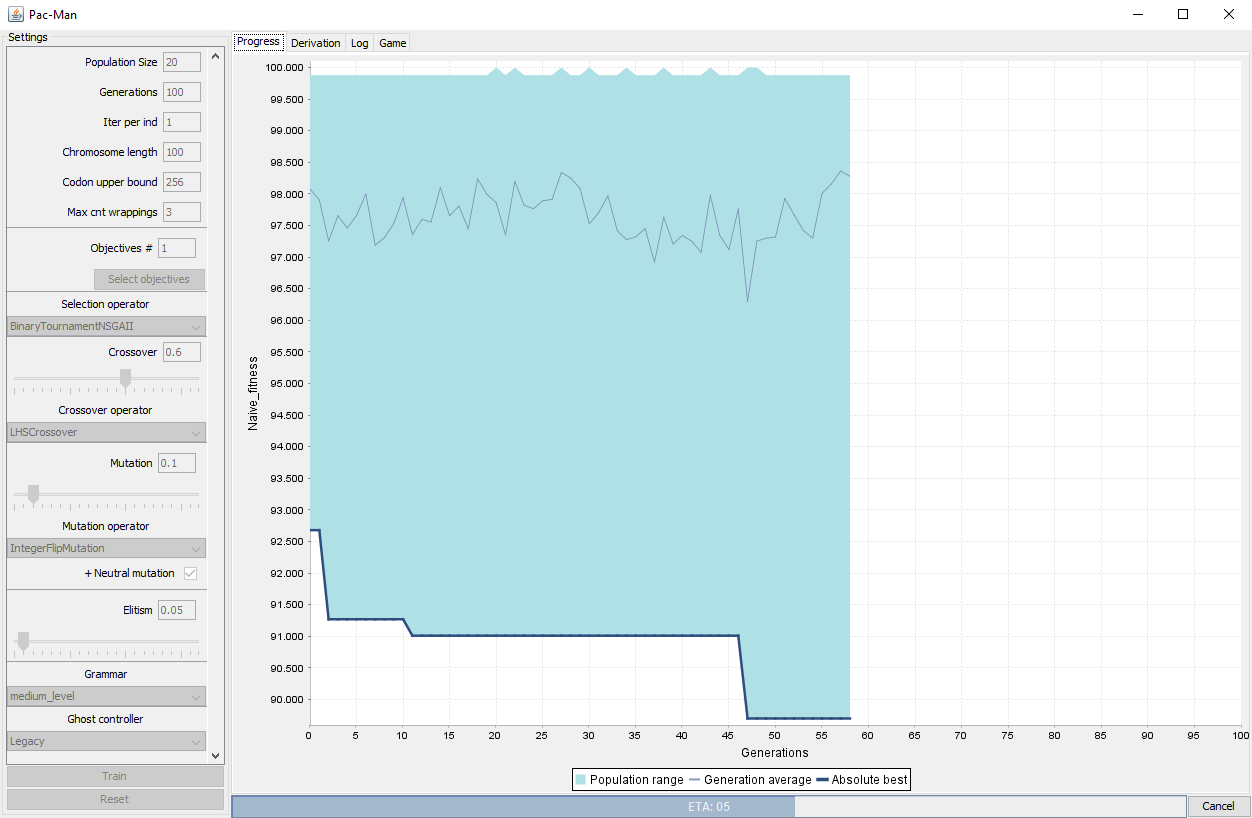
\includegraphics[width=\textwidth]{gui/portada}
\end{figure}

\section{Panel de ajustes del experimento}
A la izquierda tenemos el panel de los ajustes. Aquí se pueden modificar parámetros tanto del algoritmo evolutivo como de Pac-Man. Haremos una explicación por partes.
 
En la parte inferior izquierda pueden verse dos botones. \textit{Train} comienza la ejecución del algoritmo con los parámetros establecidos, mientras que \textit{Reset} revierte todos los parámetros a su valor por defecto.
\begin{figure}[H]
\centering
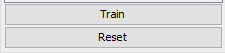
\includegraphics[width=6cm]{gui/train-reset}
\end{figure}

Una vez que finaliza la ejecución del algoritmo puede verse que aparece un botón más.
\begin{figure}[H]
\centering
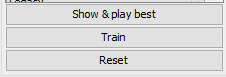
\includegraphics[width=6cm]{gui/train-reset-showplay}
\end{figure}

\textit{Show \& play best} es un atajo que cambia a la pestaña donde se ejecuta Pac-Man de manera visual, copia el fenotipo del mejor individuo en la ventana de edición y comienza la ejecución del fenotipo en el juego automáticamente.

\subsection{Parámetros del algoritmo}
Comenzando por la parte de arriba, tenemos los parámetros concretos del algoritmo de evolución gramatical.
\begin{figure}[H]
\centering
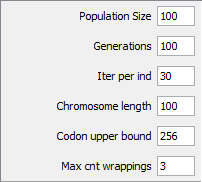
\includegraphics[width=5.5cm]{gui/parametros-algo}
\end{figure}

Con estos parámetros se pueden manejar:
\begin{itemize}
\item \textbf{\textit{Population Size}}: Tamaño de la población.

\item \textbf{\textit{Generations}}: Número de generaciones (iteraciones del algoritmo).

\item \textbf{\textit{Iter per Ind}}: Número de partidas que juega un individuo para evaluarlo.

\item \textbf{\textit{Chromosome length}}: Tamaño del cromosoma (número de codones).

\item \textbf{\textit{Codon upper bound}}: Número máximo que puede alcanzar un codón.

\item \textbf{\textit{Max cnt wrappings}}: Número máximo de \textit{wrappings} permitidos al derivar un codón.
\end{itemize}

Posteriormente tenemos el selector de objetivos del algoritmo evolutivo.
\begin{figure}[H]
\centering
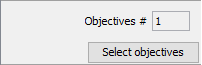
\includegraphics[width=5.5cm]{gui/objetivos}
\end{figure}

Donde ya hemos visto que se puede seleccionar la combinación de los mismos que se quiera.
\begin{figure}[H]
\centering
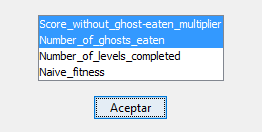
\includegraphics[width=7cm]{gui/objetivos-selector}
\end{figure}

A continuación tenemos los parámetros generales de cualquier algoritmo evolutivo: métodos de selección, operadores de cruce y operadores de mutación que se pueden seleccionar desde listas desplegables. Para el cruce y la mutación también se puede elegir la probabilidad con la que se va a aplicar el operador, la cual se puede seleccionar desde el \textit{slider} o escribir directamente en el campo de texto para mayor precisión (valores de $0$ a $1$).
\begin{figure}[H]
\centering
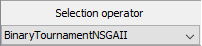
\includegraphics[width=5.5cm]{gui/seleccion}
\end{figure}
\begin{figure}[H]
\centering
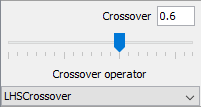
\includegraphics[width=5.5cm]{gui/cruce}
\end{figure}
\begin{figure}[H]
\centering
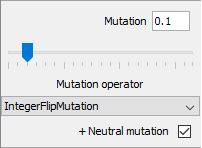
\includegraphics[width=5.5cm]{gui/mutacion}
\end{figure}

Asimismo, podemos seleccionar el porcentaje de elitismo en el algoritmo genético ya sea por \textit{slider} o campo de texto.
\begin{figure}[H]
\centering
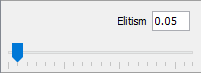
\includegraphics[width=5.5cm]{gui/elitismo}
\end{figure}

\subsection{Parámetros de Pac-Man}
Después tenemos un selector de gramáticas que el algoritmo gramatical es capaz de usar para su evolución.
\begin{figure}[H]
\centering
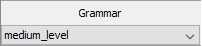
\includegraphics[width=5.5cm]{gui/grammar}
\end{figure}

Por último tenemos el controlador que los fantasmas van a usar cada vez que se juegue una partida.
\begin{figure}[H]
\centering
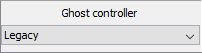
\includegraphics[width=5.5cm]{gui/ghost-controller}
\end{figure}

\section{Panel de progreso}
\begin{figure}[H]
\centering
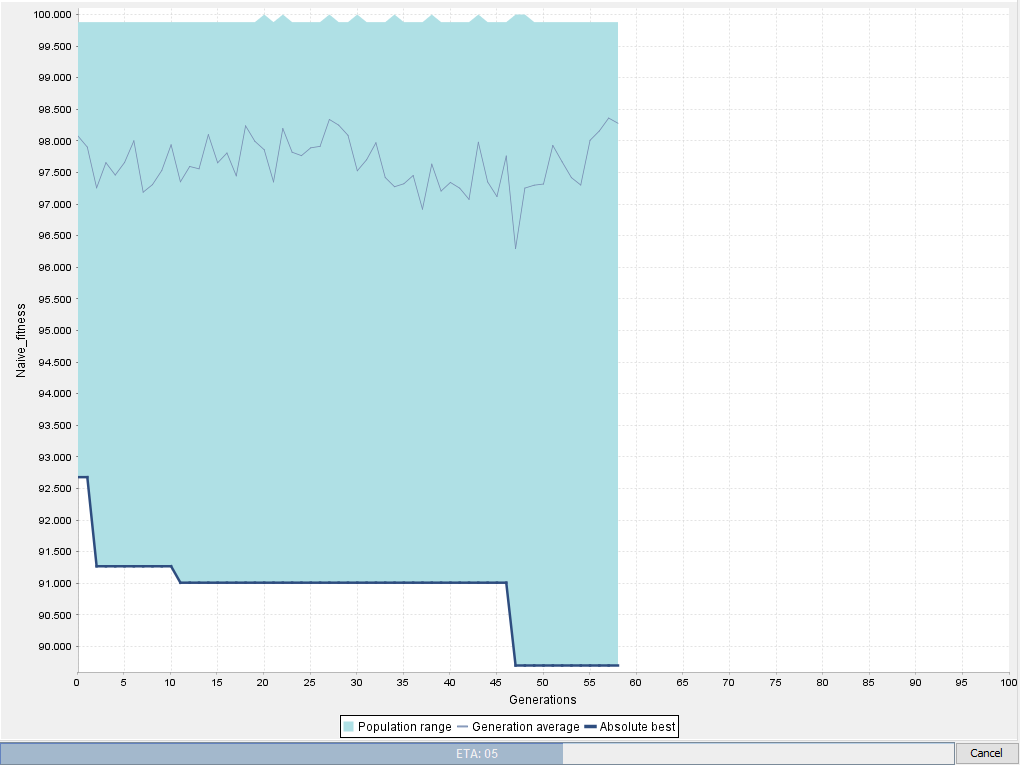
\includegraphics[width=\textwidth]{gui/progreso}
\end{figure}

Aquí vemos en tiempo real el \textit{fitness} de los individuos con cada generación, es decir, cuánto mejor se está volviendo la población. Está descendiendo porque hacemos minimización.

El eje $X$ representa el número de generaciones (iteraciones del algoritmo). El eje $Y$ son los puntos de \textit{fitness} que se están alcanzando. Si se seleccionaran dos o más objetivos, la gráfica tendría una subfigura por cada objetivo, donde se mostraría el \textit{fitness} de cada uno por separado.

La línea azul gruesa es el \textit{fitness} del mejor individuo de entre toda la población, para esa iteración del algoritmo.

La línea azul delgada indica la media del \textit{fitness} de toda la población. Con esta línea se puede discernir la puntuación global.

La franja indica el rango de \textit{fitness} en el que se mueve la población, que comprende desde el peor \textit{fitness} al mejor.

El esquema de color está inspirado en el que usa GEVA \cite{gevaGit}.

\subsection{Multiobjetivo}
También se puede visualizar el \textit{fitness} en caso de que seleccionemos más de un objetivo.
\begin{figure}[H]
\centering
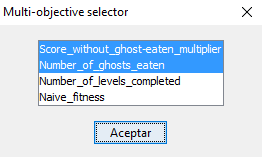
\includegraphics[width=7cm]{gui/objetivos-selector2}
\end{figure}

En ese caso se mostrarían tantas gráficas como objetivos hayamos seleccionado, teniendo cada una sus propias estadísticas para analizar la evolución de cada objetivo por separado, además de poder vislumbrar relaciones en conjunto.
\begin{figure}[H]
\centering
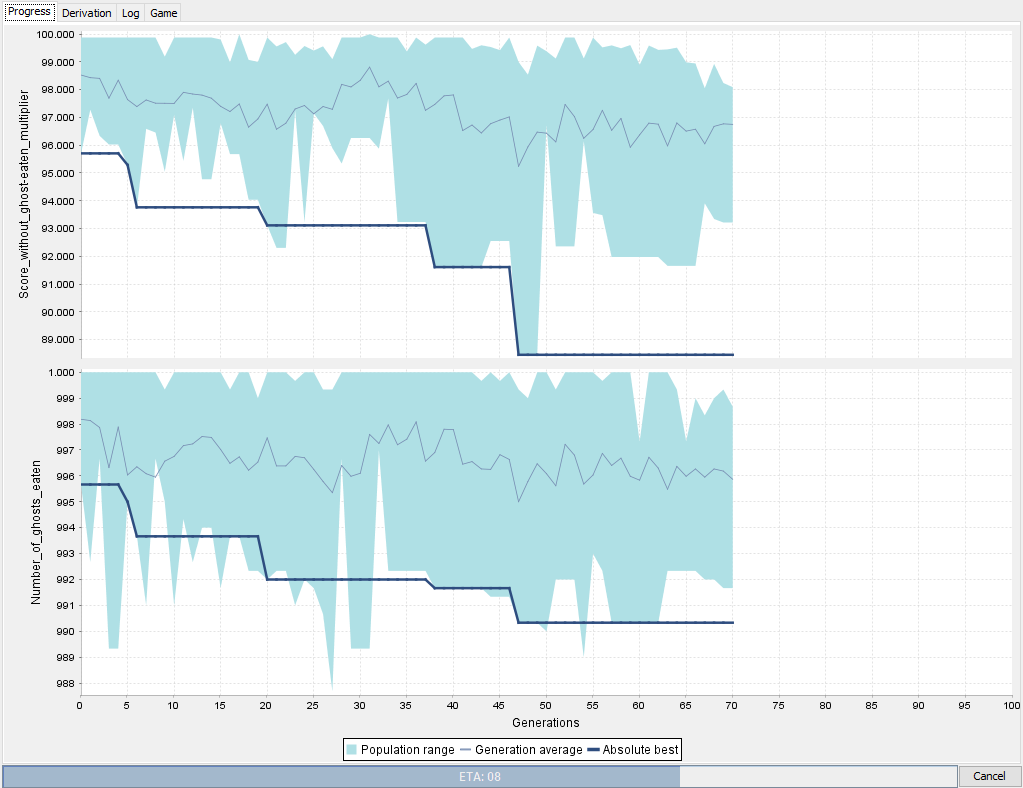
\includegraphics[width=\textwidth]{gui/multi-grafica}
\end{figure}

\subsection{Pestañas}
Tenemos varias presentaciones al mismo nivel, por lo que se han dispuesto diferentes pestañas para cambiar entre ellas. Este diseño no es limitante, permitiendo incluso analizar resultados del entrenamiento anterior mientras se está realizando un nuevo entrenamiento.
\begin{figure}[H]
\centering
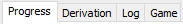
\includegraphics[width=7cm]{gui/pestanas}
\end{figure}

\subsection{Tiempo estimado}
Este panel también cuenta con una barra de progreso que aparece durante la ejecución y desaparece al terminar. Indica además el tiempo estimado restante en una etiqueta sobre la barra. Esta barra también cuenta con un botón \textit{Cancel} para detener la ejecución del algoritmo en cualquier punto del entrenamiento, pudiendo hacer análisis de la evolución y ejecuciones del mejor individuo hasta el momento de la parada.
\begin{figure}[H]
\centering

\includegraphics[width=\textwidth]{gui/barra-progreso}
\end{figure}

\section{Panel del mejor individuo}
En cuanto el algoritmo termina de entrenar aquí podemos ver el fenotipo correspondiente al mejor individuo.
\begin{figure}[H]
\centering
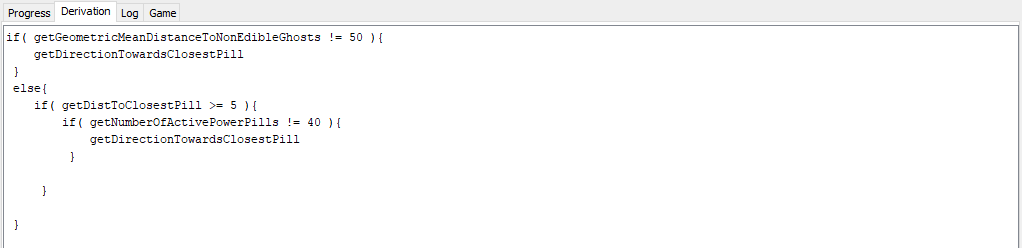
\includegraphics[width=\textwidth]{gui/derivation}
\end{figure}

\section{Panel de juego}
Permite ejecutar y analizar visualmente una partida del juego \textit{Ms. Pac-Man} a partir de un fenotipo dado.

El botón \textit{Copy best here} copia el programa del mejor individuo generado por el algoritmo a la ventana de edición, para después ejecutarlo directamente en Pac-Man con el botón \textit{Run code} o editarlo antes de ejecutar, si se desea.

Los controles contienen además un slider que permite ajustar la velocidad de la partida dentro de un rango razonable.
\begin{figure}[H]
\centering
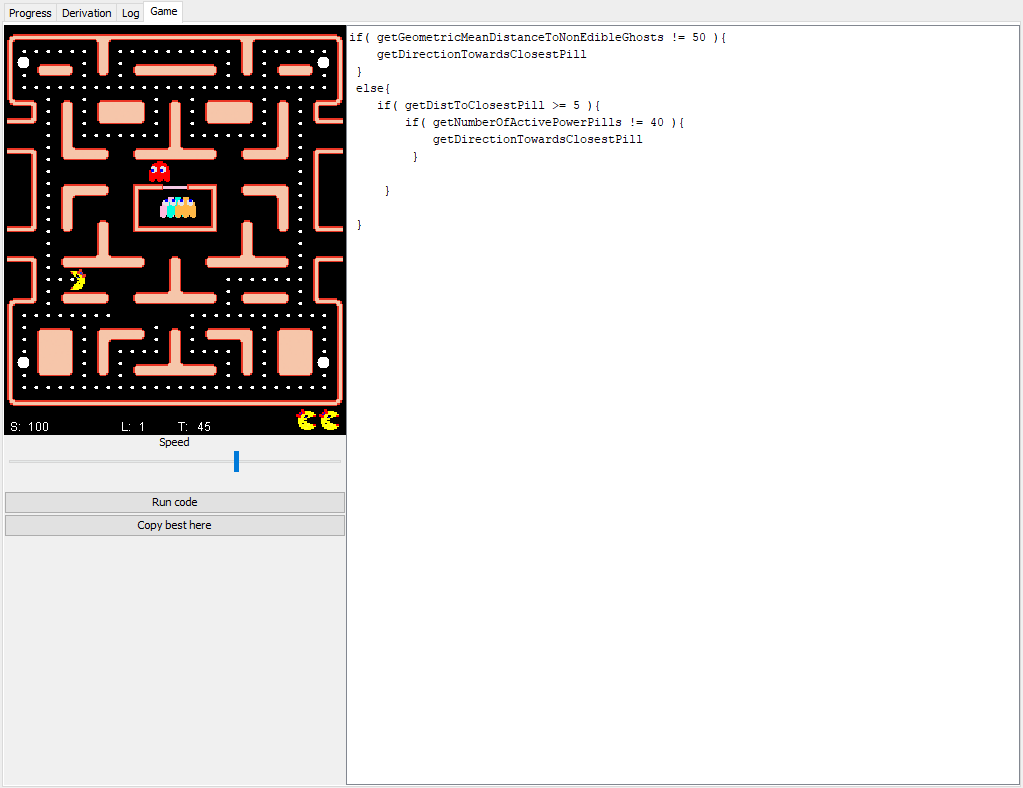
\includegraphics[width=\textwidth]{gui/game}
\end{figure}

\chapter{Conclusiones}

\section{Conclusiones}
A lo largo del desarrollo del Trabajo de Fin de Grado hemos pasado por numerosas versiones con distintos enfoques aplicados a la generación de bot de Ms. Pac-Man a través de gramáticas evolutivas. 
 
Primero de todo, mediante la generación de autómatas que ejecutaban cadenas de acciones (que posteriormente fue ampliado con acciones de más alto nivel y condicionales muy simples), que, si bien no alcanzó resultados destacablemente positivos, si logró encontrar una brecha en las reglas del juego que le permitía conseguir completar niveles muy fácilmente contra fantasmas no muy inteligentes.
 
Después, orientamos nuestra gramática a la generación de controladores reactivos, sustituyendo también las anteriores cadenas de acciones por un árbol de decisión. Este cambio supuso una mejora significativa, permitiéndonos diseñar gramáticas de distintos niveles de abstracción.
 
A continuación, realizamos una serie de estudios (de la presión selectiva, del uso de codones y de funciones de fitness) que nos llevaron a incluir numerosas mejoras con el fin de mejorar tanto los resultados obtenidos por el algoritmo evolutivo (cruce LHS, Mutación Neutral, optimización multiobjetivo y numerosos cambios menores en el framework JECO), como la comodidad de empleo de la herramienta (multithread). Todas estas mejoras centradas en el algoritmo evolutivo han tenido la suficiente repercusión en el rendimiento de los bots generados como para formar parte de los parámetros con los que alcanzamos mejores resultados.
 
Finalmente, tras un profundo análisis de todas las diferentes pruebas que hemos realizado durante el transcurso de Trabajo de Fin de Grado, podemos concluir con una serie de hechos. 
 
Primero de todo, obtenemos los mejores resultados, tanto para cualquier gramática como para cualquier controlador de fantasmas adversario, utilizando los siguientes parámetros del algoritmo evolutivo:
\begin{table}[H]
\centering
\begin{tabular}{lcc}
\cline{3-3}
                                                   &                                                               & \textbf{Porcentaje} \\ \cline{3-3} 
\multicolumn{1}{|l|}{\textbf{Método de selección}} & Torneo Binario \footnotemark & -                   \\
\multicolumn{1}{|l|}{\textbf{Método de cruce}}     & LHS                                                           & 60                  \\
\multicolumn{1}{|l|}{\textbf{Método de mutación}}  & Integer Flip                                                  & 10                  \\
\multicolumn{1}{|l|}{\textbf{Mutación Neutral}}    & Sí                                                            & -                   \\
\multicolumn{1}{|l|}{\textbf{Elitismo}}            & Sí                                                            & 5                  
\end{tabular}
\end{table}
\footnotetext{o NSGA II si se está empleando multiobjetivo}
\begin{figure}[]
\centering
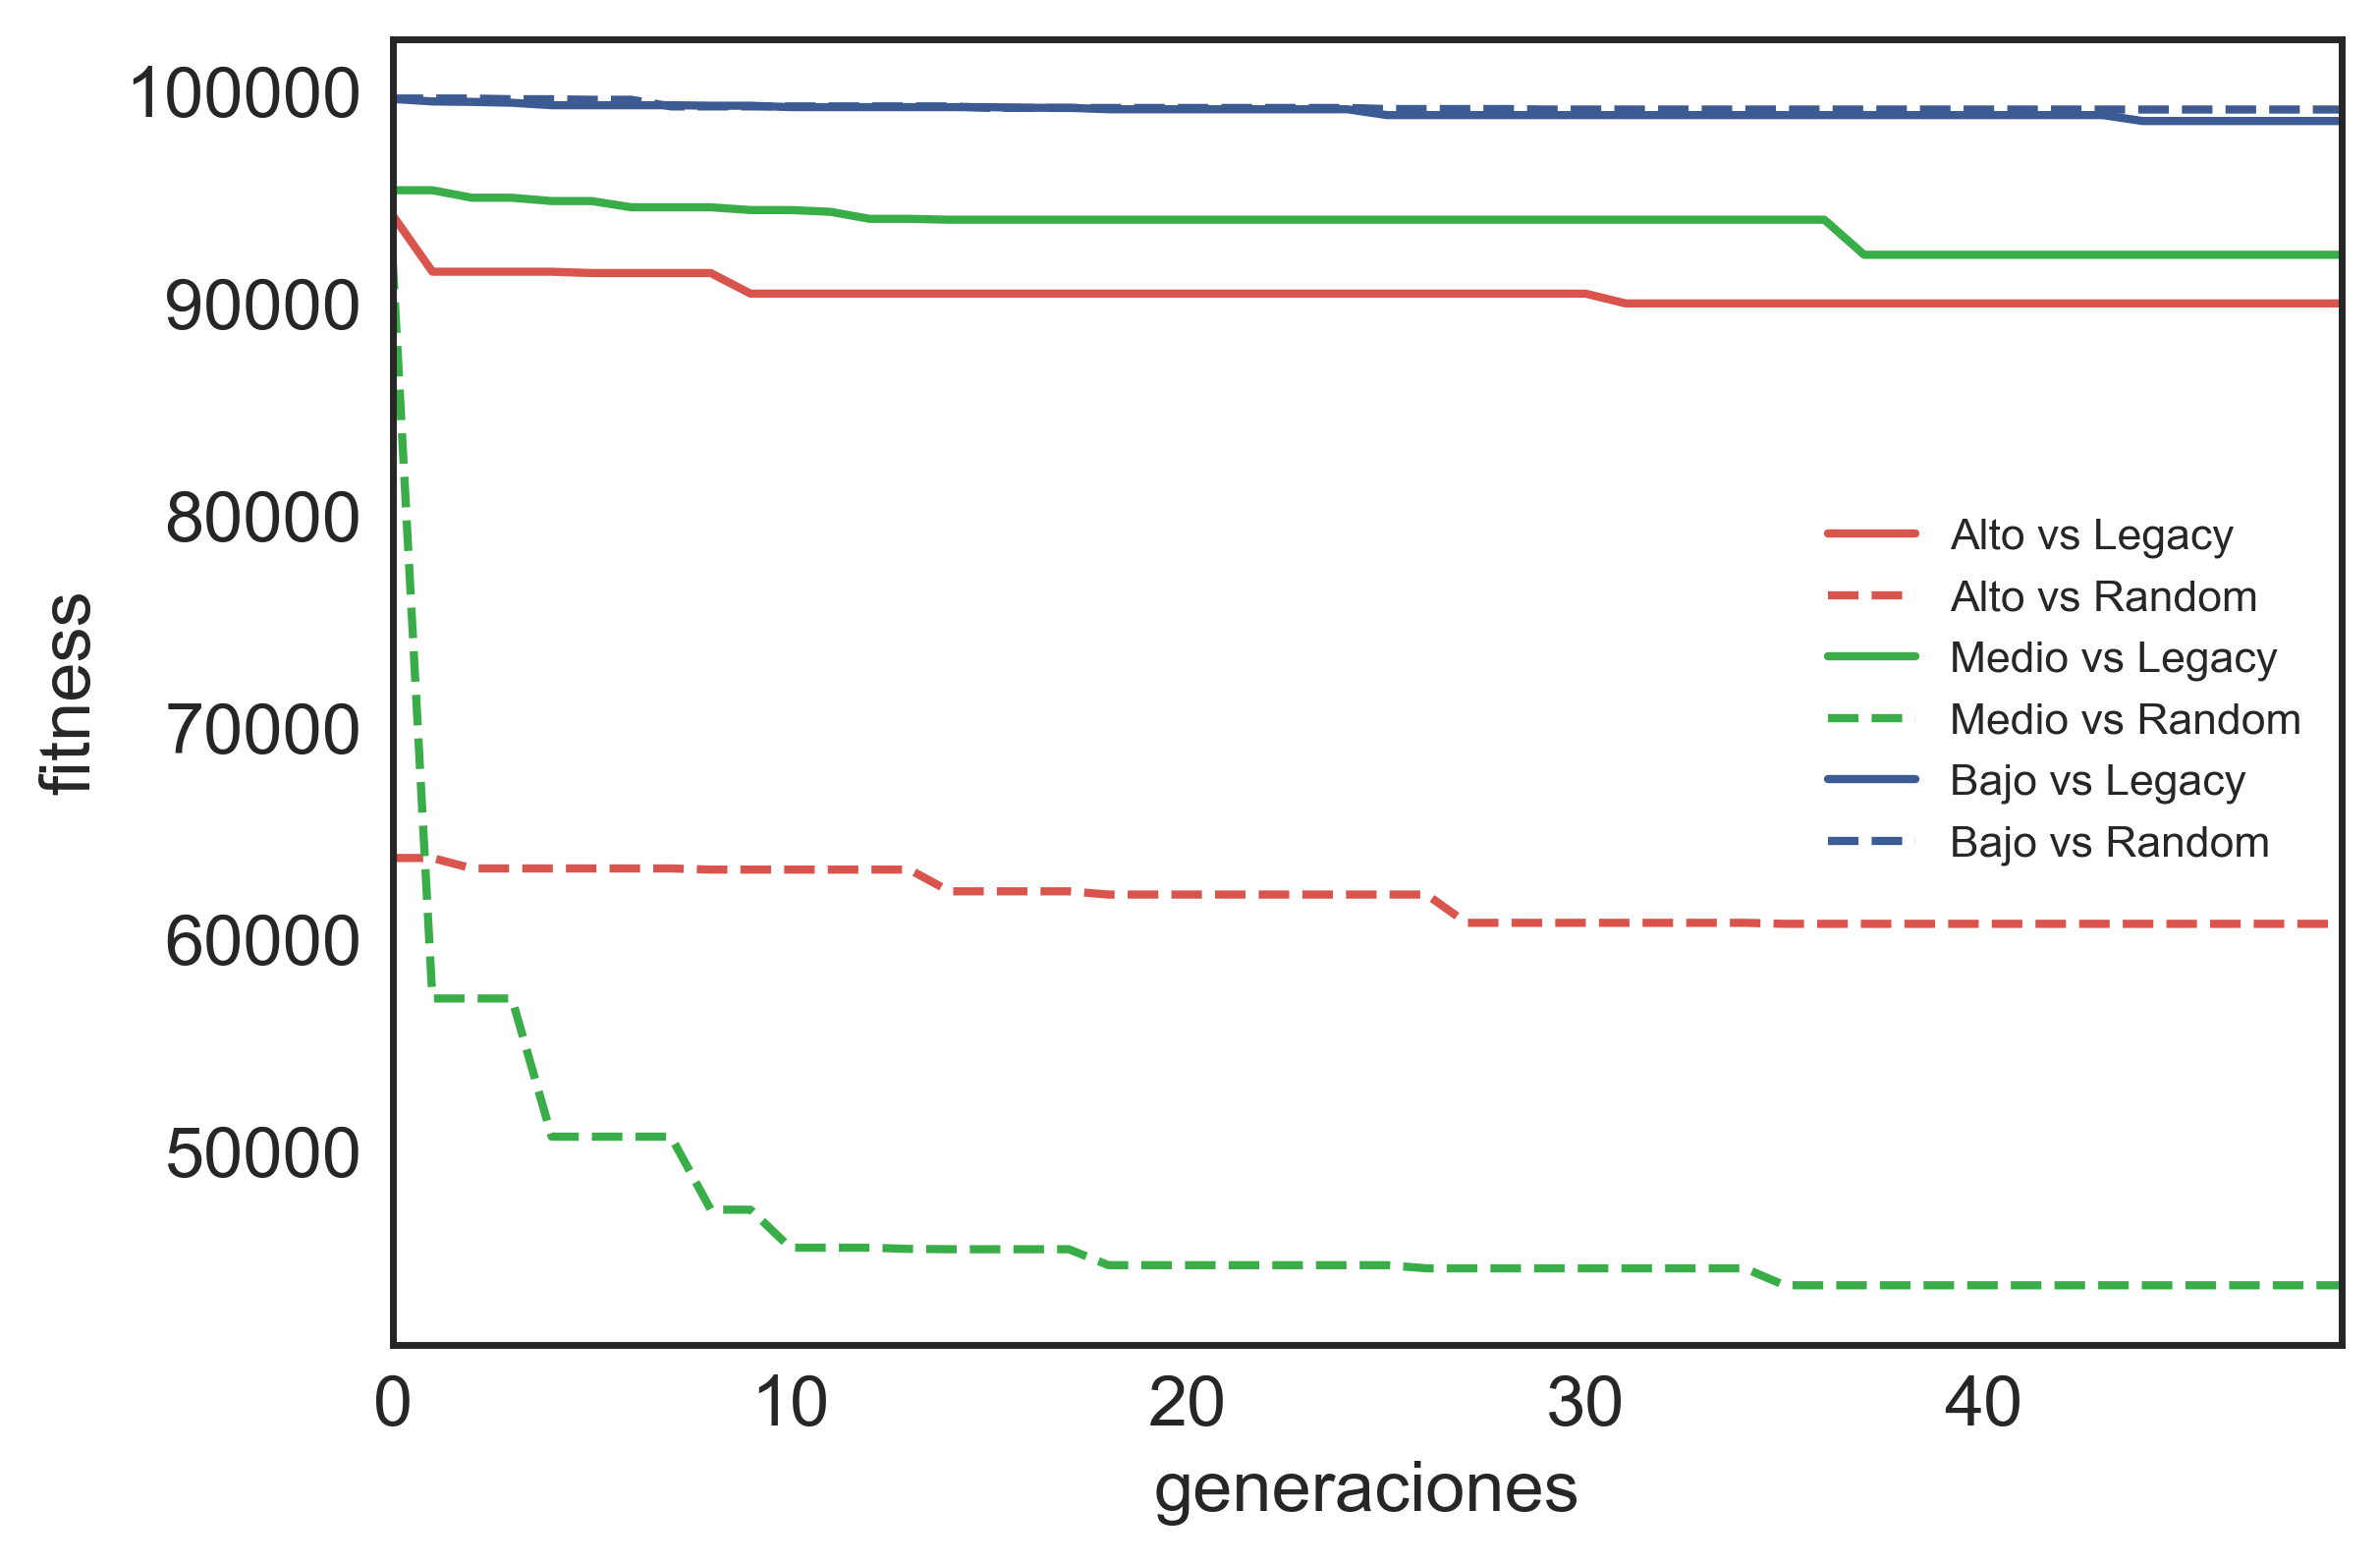
\includegraphics[width=0.8\textwidth]{grafica/all_fitnesses}
\label{graph:all_fitness}
\caption{\textit{Fitness} con un solo objetivo.}
\end{figure}

Segundo, tal como se aprecia se en la Figura~\ref{graph:all_fitness}, los bots consiguen mejores resultados en evoluciones con pocas generaciones, 50 en el caso de la gráfica, cuanto mayor es la abstracción de la gramática aplicada. No obstante, los bots generados usando la gramática de medio nivel consiguen superar a los de alto nivel con muchas generaciones (por ejemplo 100), al tener mayor potencial, como se explica más adelante en la Tabla~\ref{table:single_obj}.
 
Tercero, tal como se aprecia en la Tabla~\ref{table:single_obj}, los bots generados usando tanto la gramática de medio nivel como la de alto nivel superan los controladores de Pac-Man base así como otros bots generados por gramáticas evolutivas, como por ejemplo el generado por la universidad UCD de Dublín. Esto ocurre tanto enfrentándose al controlador \textit{Random Ghosts} como al de \textit{Legacy Ghosts}.
 
Uno de los factores que nos permiten obtener mejores resultados que el bot \cite{galvan2010evolving} de UCD Dublin (especialmente interesante al estar también basado en gramáticas evolutivas) consiste en que su bot emplea funciones demasiado específicas, las cuales acaban limitando el comportamiento del bot, siendo una de ellas por ejemplo esperar a que los fantasmas se acerquen siempre que se encuentre al lado de una \textit{power pill}. 
Otro de los factores es el uso de numerosos parámetros para evaluar sus funciones condicionales. Por ejemplo, su bot utiliza una ventana alrededor de Pac-Man, dentro de la cual evalúa condiciones como encontrar fantasmas dentro de esta. Para emplear dicha ventana, emplea dos parámetros ancho y alto. Por otro lado, nuestras funciones condicionales obtienen directamente la distancia de la ruta a determinados elementos, pudiendo operar esta distancia con distintos operadores numéricos sobre valores también numericos.
\begin{table}[]
\centering
\label{table:single_obj}
\begin{tabular}{|l|c|r|r|r|r|r|r|r|r|r|}
\hline
\multicolumn{1}{|c|}{\multirow{2}{*}{\textbf{Pac-Man}}} & \multirow{2}{*}{\textbf{Ghosts}} & \multicolumn{3}{c|}{\textbf{score}} & \multicolumn{3}{c|}{\textbf{level}} & \multicolumn{3}{c|}{\textbf{time (game ticks)}} \\ \cline{3-11} 
\multicolumn{1}{|c|}{} &  & \multicolumn{1}{c|}{\textbf{max}} & \multicolumn{1}{c|}{\textbf{avg}} & \multicolumn{1}{c|}{\textbf{std}} & \multicolumn{1}{c|}{\textbf{max}} & \multicolumn{1}{c|}{\textbf{avg}} & \multicolumn{1}{c|}{\textbf{std}} & \multicolumn{1}{c|}{\textbf{max}} & \multicolumn{1}{c|}{\textbf{avg}} & \multicolumn{1}{c|}{\textbf{std}} \\ \hline
Random &  \multirow{5}{*}{Random} & 1380 & 501 & 213 & 1 & 0.036 & 0.186 & 5635 & 1943 & 887.5 \\ \cline{1-1} \cline{3-11} 
NearestPill &  & 18910 & 4471 & 2654 & 5 & 1 & 0.9 & 7216 & 1795 & 1018 \\ \cline{1-1} \cline{3-11} 
UCD Dublin bot \cite{galvan2010evolving} &  & 11640 & 4288 & - & - & - & - & - & - & - \\ \cline{1-1} \cline{3-11} 
\textbf{Low-level} &  & \textbf{900} & \textbf{151} & \textbf{117} & \textbf{1} & \textbf{0.071} & \textbf{0.257} & \textbf{5094} & \textbf{2151} & \textbf{972.1} \\ \cline{1-1} \cline{3-11} 
\textbf{Medium-level} &  & \textbf{64600} & \textbf{48558} & \textbf{10780} & \textbf{18} & \textbf{15} & \textbf{3.4} & \textbf{24000} & \textbf{21579} & \textbf{4470} \\ \cline{1-1} \cline{3-11} 
\textbf{High-level} &  & \textbf{55480} & \textbf{32704} & \textbf{13237} & \textbf{18} & \textbf{10.4} & \textbf{4.3} & \textbf{24000} & \textbf{17457} & \textbf{6784} \\ \hline
Random & \multirow{5}{*}{Legacy} & 1840 & 197 & 107 & 0 & 0 & 0 & 877 & 465 & 61.3 \\ \cline{1-1} \cline{3-11} 
NearestPill &  & 7190 & 3531 & 638 & 1 & 0.4 & 0.5 & 1881 & 1152 & 143.7 \\ \cline{1-1} \cline{3-11} 
UCD Dublin bot \cite{galvan2010evolving} &  & 12350 & 3945 & - & - & - & - & - & - & - \\ \cline{1-1} \cline{3-11} 
\textbf{Low-level} &  & \textbf{120} & \textbf{120} & \textbf{0} & \textbf{0} & \textbf{0} & \textbf{0} & \textbf{600} & \textbf{425} & \textbf{34.5} \\ \cline{1-1} \cline{3-11} 
\textbf{Medium-level} &  & \textbf{15960} & \textbf{6358} & \textbf{2883} & \textbf{3} & \textbf{0.9} & \textbf{0.7} & \textbf{4973} & \textbf{1916} & \textbf{730} \\ \cline{1-1} \cline{3-11} 
\textbf{High-level} &  & \textbf{20040} & \textbf{5972} & \textbf{2832} & \textbf{4} & \textbf{1} & \textbf{0.6} & \textbf{8364} & \textbf{2026} & \textbf{1020} \\ \hline
\end{tabular}
\caption{Pac-Man vs Ghost controllers' comparison.}
\end{table}

Por último, si bien el empleo de la optimización multiobjetivo supone una mejora significativa en ejecuciones del algoritmo evolutivo relativamente cortas (al evitar estancamiento en los numerosos mínimos locales), no produce una diferencia suficientemente significativa en los bots generados mediante ejecuciones suficientemente largas. Esto es apreciable en la Tabla~\ref{table:multi-objective} (donde las sigles MO se refieren a los bots que emplean la Optimización Multiobjetivo), y sucede así en el caso concreto de Ms. Pac-Man vs Ghost debido a la relación directa entre los distintos fitness que hemos perseguido en multiobjetivo (fantasmas comidos, niveles completados y puntos alcanzados sin el multiplicador de puntos al comer fantasmas) con la puntuación (fitness perseguido previo a la optimización multiobjetivo), siendo esta una composición de los fitness anteriores.
\begin{table}[tb]
\centering
\label{table:multi-objective}
\begin{tabular}{|l|c|r|r|r|r|r|r|r|r|r|}
\hline
\multicolumn{1}{|c|}{\multirow{2}{*}{\textbf{Pac-Man}}} & \multirow{2}{*}{\textbf{Ghosts}} & \multicolumn{3}{c|}{\textbf{score}} & \multicolumn{3}{c|}{\textbf{level}} & \multicolumn{3}{c|}{\textbf{time (game ticks)}} \\ \cline{3-11} 
\multicolumn{1}{|c|}{} &  & \multicolumn{1}{c|}{\textbf{max}} & \multicolumn{1}{c|}{\textbf{avg}} & \multicolumn{1}{c|}{\textbf{std}} & \multicolumn{1}{c|}{\textbf{max}} & \multicolumn{1}{c|}{\textbf{avg}} & \multicolumn{1}{c|}{\textbf{std}} & \multicolumn{1}{c|}{\textbf{max}} & \multicolumn{1}{c|}{\textbf{avg}} & \multicolumn{1}{c|}{\textbf{std}} \\ \hline
Medium-level \ref{table:single_obj} & \multirow{4}{*}{Random} & {64600} & {48558} & {10780} & {18} & {15} & {3.4} & {24000} & {21579} & {4470} \\ \cline{1-1} \cline{3-11} 
\textbf{Medium-level (MO)} &  & \textbf{62050} & \textbf{46922} & \textbf{1243} & \textbf{18} & \textbf{15} & \textbf{4} & \textbf{24000} & \textbf{20868} & \textbf{5094.5} \\ \cline{1-1} \cline{3-11} 
{High-level \ref{table:single_obj}} &  & {55480} & {32704} & {13237} & {18} & {10.4} & {4.3} & {24000} & {17457} & {6784} \\ \cline{1-1} \cline{3-11} 
\textbf{High-level (MO)} &  & \textbf{57370} & \textbf{32441} & \textbf{12712} & \textbf{17} & \textbf{10} & \textbf{4.1} & \textbf{24000} & \textbf{17536} & \textbf{6604.7} \\ \hline
{Medium-level \ref{table:single_obj}} & \multirow{4}{*}{Legacy} & {15960} & {6358} & {2883} & {3} & {0.9} & {0.7} & {4973} & {1916} & {730} \\ \cline{1-1} \cline{3-11} 
\textbf{Medium-level (MO)} &  & \textbf{18020} & \textbf{6229} & \textbf{2832} & \textbf{3} & \textbf{0.9} & \textbf{0.7} & \textbf{5041} & \textbf{1905} & \textbf{725} \\ \cline{1-1} \cline{3-11} 
{High-level \ref{table:single_obj}} &  & {20040} & {5972} & {2832} & {4} & {1} & {0.6} & {8364} & {2026} & {1020} \\ \cline{1-1} \cline{3-11} 
\textbf{High-level (MO)} &  & \textbf{20040} & \textbf{5972} & \textbf{2832} & \textbf{4} & \textbf{1} & \textbf{0.6} & \textbf{8364} & \textbf{2026} & \textbf{1020} \\ \hline
\end{tabular}
\caption{Pac-Man vs Ghost controllers' comparison including Multi-Objective.}
\end{table}


\section{Difusión}
Considerando el impacto que puede tener el proyecto que hemos realizado, hemos decidido publicarlo \cite{thesisGit} como código abierto y bajo licencia GPL \cite{licenseThesisGit} en la plataforma GitHub. Esto lo hicimos con la esperanza de poder ser de ayuda a cualquier proyecto relacionado con el campo de la evolución gramatical o la inteligencia artificial aplicada a videojuegos

Finalmente, una vez habíamos obtenido y analizado los resultados del proyecto, decidimos llevarlo un paso mas allá y publicar un artículo científico sobre él. Este, titulado ``A Pac-Man bot based on Grammatical evolution'', se centra en la implementación final (arboles de decisión) y el uso de gramáticas de medio y alto nivel, mencionando brevemente la mejora de optimización multiobjetivo. En estos momentos el artículo ha sido enviado al CoSECiVi 2017 (Congreso de la Sociedad Española para las Ciencias del Videojuego) y se encuentra pendiente de revisión por pares.

\section{Trabajo futuro}
Aunque estamos satisfechos con el alcance de nuestro trabajo y sus resultados, nos habría gustado experimentar y comprobar otras técnicas no incluidas por falta de tiempo. Son las que se describen a continuación.

\subsection{Árboles de comportamiento}
Una de las posibles técnicas a aplicar son los árboles de comportamiento (\textit{Behaviour trees}). 
El uso de árboles de comportamiento habría supuesto incluir en nuestras gramáticas bucles en los formatos típicos (\texttt{while, for, do-while}, ...). Esto supone que para encontrar un terminal que devuelva un movimiento en nuestro árbol de decisión, ya no se parte siempre desde la raíz, sino que puede tener que continuarse en un punto definido por las solicitudes de movimiento previas.

Esta técnica en principio posibilita, o facilita la producción de estrategias más específicas, que requieran continuidad. Sin árboles de comportamiento también pueden conseguirse, pero el conjunto de condiciones a evaluar para llegar a dichas estrategias y soportar varias a la vez puede hacerse enorme, y llegar a dichas soluciones en un espacio de búsqueda tan grande/complejo es extremadamente poco factible en términos de potencia computacional.

\subsection{NEAT}
Otra técnica prometedora sería la aplicación de redes neuronales debido a su amplio espectro y gran capacidad de generalización.

Como \textit{input}s tendríamos las mismas funciones de las que hacen uso las gramáticas para conocer el estado del juego y como \textit{output} nos daría un movimiento que ejecutaría Pac-Man.

El problema radicaría en la arquitectura de la red, por lo que para dar con la óptima y siguiendo con el espíritu evolucionista, usaríamos el algoritmo NEAT \cite{stanley2002evolving} (\textit{NeuroEvolution of Augmenting Topologies}). Este algoritmo se vale de técnicas de Programación Evolutiva para evolucionar y proteger las topologías de las redes neuronales que genera hasta que están lo suficientemente entrenadas para resolver con éxito un problema concreto. La ventaja adicional es que se podría integrar dentro del framework JECO con mínimo esfuerzo, más allá de la implementación del mismo.
\chapter{Conclusions}
All along this undergraduate thesis we have iterated through numerous versions with different approaches, all applied to the generation of our bot for Ms. Pac-Man with grammatical evolution.
 
First of all, with the automaton approach, the bot executed sequences of actions (which was later improved with high level actions and very simple conditional evaluations), even if it’s results weren’t so good score-wise, achieved to develop a tactic that allowed it to progress many levels against the most silly ghosts.
 
After that we oriented our grammars to follow a reactive approach, changing our previous sequences of actions for decision trees. This change was a significative breakthrough, that allowed us to design grammars with different levels of abstraction.
 
Next, we did a series of studies (of selective pressure, codon usage, and fitness functions) which lead us numerous improvements in a try to obtain better results, both in algorithm efficacy (LHS cross-over, neutral mutation, multi-objective optimization, and multiple minor changes to the JECO framework), and the friendliness of our tool (multithreading). All this upgrades had enough repercussion in the bot performance as to include them in the parameters of execution for the best results we show.
 
Finally, after analysing all the tests we did, we could conclude various things.
 
First of all, we obtain the best results, for any grammar and against any ghost controller, using the following parameters for the evolutive algorithm:
\begin{table}[H]
\centering
\begin{tabular}{lcc}
\cline{3-3}
                                                   &                                                               & \textbf{Percentage} \\ \cline{3-3} 
\multicolumn{1}{|l|}{\textbf{Selection operator}} & Binary tournament \footnotemark & -                   \\
\multicolumn{1}{|l|}{\textbf{Crossover operator}}     & LHS                                                           & 60                  \\
\multicolumn{1}{|l|}{\textbf{Mutation operator}}  & Integer Flip                                                  & 10                  \\
\multicolumn{1}{|l|}{\textbf{Neutral Mutation}}    & Yes                                                            & -                   \\
\multicolumn{1}{|l|}{\textbf{Elitism}}            & Yes                                                            & 5                  
\end{tabular}
\end{table}
\footnotetext{or NSGA II if multi-objective is being used}

Second, as Figure~\ref{graph:all_fitness} shows, the bots obtain better results, when using only a few generations (for example 50), as the more abstract the used grammar is. However, when using more generations (for example 100), the bots using the medium-level grammar obtain the best results, due to its higher potencial, as shown later at Table~\ref{table:single_obj}.
 
Third, as Table~\ref{table:single_obj} shows, our grammars can produce bots that play better than the baseline controllers (a random controller and other one that always goes towards the closest pill). Besides, our bots play better than the UCD Dublin bot \cite{galvan2010evolving}, and that is interesting because all of them are created using Grammatical Evolution. This seems to happen due to the usage of excessively specific functions which limit its behaviour, i.e. forcing Pac-Man to wait next to a power pill. Their bot also uses large amount of parameters like dimensions of a frame (centered on Pac-Man) to evaluate certain conditions. Conversely, we make use of path distances and numeric operators, resulting in a less complex game status analysis.

Lastly, even if the use of multi-objective optimization makes short executions obtain slightly better results (it helps to avoid local minimums), it doesn’t obtain a significative difference in long enough executions, as Table~\ref{table:multi-objective} shows (where MO means that the bot uses Multiobjetive Optimization). This happens in Ms. Pac-Man vs Ghosts due to the direct relation between the different fitnesses which can be applied (ghosts eaten, levels cleared..) and the overall game score, which is based on all those.

\chapter{Contribuciones individuales} \label{cap:contribuciones}

\section{Héctor Laria Mantecón}
Decidir la versión de Pac-Man a utilizar fue bastante fácil ya que nuestro profesor Antonio nos recomendó una con bastantes buenas referencias, así que pudimos jugar todos en verano con ella para entenderla bien. Cuando empezó el curso buscamos el \textit{framework} de Programación Evolutiva, probando primeramente con GEVA. Ninguno consiguió hacerlo funcionar porque usaba tecnología un poco obsoleta y era algo oscuro. Así que nuestro profesor Carlos nos presentó una segunda opción en la que estábamos de acuerdo los cuatro, JECO. Ésta era más simple, versátil y mejor organizada así que aunque todos hemos tenido que pelear y modificarla en algún momento, nos ha sido de mucha utilidad.

Teniendo eso resuelto, lo primero que hice fue encargarme del repositorio de código ya que yo estaba más familiarizado con el uso de herramientas de versionado, desarrollo en ramas, \textit{issues}, uso de etiquetas y versiones, etc. Puse a disposición de los demás algunas páginas en la \textit{wiki} del repositorio sobre cómo borrar y fusionar ramas y demás. Tampoco fue la panacea, ya que aprendimos a las malas que el desarrollo paralelo es mejor dividirlo por \textit{features}, no por personas.

Una vez dominado y debido al buen funcionamiento que llevábamos, pensamos en ir un poco más allá y buscar una herramienta de gestión de proyectos más avanzada y que tuviera integración con nuestro repositorio de \textit{GitHub}. Sobre todo porque en ese momento había ciertas tareas que requerían de otras y no queríamos dejar a gente parada. Busqué e hice comparación de herramientas sobre todo con diagramas de \textit{Gantt} y encontré algunas pero de todas las que había no había ninguna que no fuese de pago. Al final llegó un momento en que tuvimos material suficiente como para que ninguno tuviese que estar esperando y dejamos la idea de estas herramientas a un lado.

En lo referente a la implementación, después de que Jorge Vieira conectara la versión del autómata con Pac-Man conseguí junto a él activar el multihilo para el algoritmo evolutivo y nos quedamos impresionados por el rendimiento que nos daba, ahora podíamos hacer uso de operadores más complejos y aumentar el tamaño de la evolución tardando incluso menos tiempo.

Más tarde, añadí soporte para funciones de \textit{fitness} en JECO para mayor modularidad y que nos fuera más fácil cambiar entre funciones, con vistas al futuro.

Cuando terminamos el autómata estaba claro que necesitábamos una definición mejor de gramática y una conexión mejor con la ejecución en Pac-Man. Era el único que no había dado fundamentos ni procesamiento de lenguaje, así que me propuse investigar y aprender sobre gramáticas, sacando al final la llamada gramática base. A la que además le pude meter las funciones en las que estaban trabajando los demás. Cuando la terminé tuvo muy buena aceptación y me dieron \textit{feedback} para pulir ciertos detalles. Estoy muy contento con esa gramática porque es muy robusta y bien organizada, así que nos sirvió como base para todas las siguientes gramáticas que se hicieron, cumpliendo totalmente mi objetivo.

Después de que José Miguel implementara los árboles de decisión que íbamos a usar para ejecutar el controlador de Pac-Man, me ocupé de que JECO derivara programas de la gramática base para después pasar el string producido al constructor de árboles José Miguel. Corregimos los fallos que nos daba el \textit{parseo} y así finalmente habíamos conectado JECO con los árboles de derivación.

Seguidamente, hice el código para ejecutar esos árboles en Pac-Man y que devolvieran un movimiento cada vez que se le pedía desde el juego, cerrando así el círculo con el algoritmo evolutivo, al conectar los árboles de derivación con Pac-Man. Más tarde esta parte sería reescrita para usar una nueva implementación de árbol más clara.

Paralelamente al desarrollo del trabajo, me ocupé en solitario de crear una interfaz gráfica que fuera sencilla y cubriera todas nuestras necesidades. Si tuviera que hacerla de nuevo me negaría en rotundo a hacerla yo solo, lo distribuiríamos entre dos o entre los cuatro. Tuve la suerte de empezar en vacaciones de navidad pero fue un trabajo demasiado grande, tanto como para empezar como para mantenerla y actualizarla.

Tuve que modificar los algoritmos de JECO, los patrones que implementaba, hacer una arquitectura entera para hablar con todas las partes, investigar la librería gráfica de Java para que no se bloqueara la interfaz al evolucionar, además conseguir que el multiobjetivo siguiera funcionando a la vez, investigar librerías de dibujado de gráficas, investigar la implementación de Pac-Man para incrustar su ventana en la interfaz, sin que se bloqueara tampoco al ejecutar una partida ni al estar evolucionando, y un largo etcétera de problemas que surgieron más adelante.
En los últimos meses estaba tan ocupado que José Miguel me echó una mano para añadir ciertos detalles, como el selector de \textit{fitness} multiobjetivo.

Después de terminar los árboles llegó la hora de empezar a experimentar con multiobjetivo. Después de consultar y ver que JECO tenía soporte y los operadores necesarios para ello, me dispuse a mejorar la primera versión del soporte de \textit{fitness} que había hecho antes para que soportara varios \textit{fitness} a la vez, pasándole a JECO los resultados fácilmente.
En los últimos meses, gracias al sistema gestor de recursos que hizo Jorge Vieira pude tener suficientes datos para hacer varios análisis de los entrenamientos, además de sacar gráficas y estadísticas tanto para el artículo como la memoria. Usé \textit{Jupyter Notebook} y las librerías \textit{Pandas} y \textit{Seaborn} para ello.

Siguiendo con los análisis, debido a la naturaleza estocástica de los controladores de los fantasmas, necesitábamos tantos datos como fuera posible para paliar este efecto y poder hacer mediciones correctas. Por lo que hice un \textit{script} que corría miles de partidas y guardaba los datos. José Miguel me ayudó a manejar los datos y conseguimos las medidas de los mejores elementos de las evoluciones, con mucho mayor detalle que en el entrenamiento.

En definitiva, he aprendido mucho con este trabajo. Cómo trabajar en equipo (mucho más que en la carrera), cómo hacer las cosas, cómo no hacerlas, lo fácil que es acostumbrarse al buen trabajo de los compañeros y más. También he aumentado mis conocimientos Programación Evolutiva y, por lo menos yo, le he cogido el gusto a leer artículos de investigación.

\section{Jorge Sánchez Cremades}
Nuestro profesor Antonio antes de comenzar el curso nos facilitó el código de una versión del juego Pac-Man que es utilizada normalmente en competiciones y desarrollo de Inteligencia Artificial. Durante el verano tuvimos tiempo de experimentar con esta versión y ver su funcionamiento interno (controladores de Pac-Man, controladores de Fantasmas, modos de ejecución del juego, lógica interna, etc.) y pensar cómo se podría adaptar para su uso en un algoritmo evolutivo.

Debido a mi estancia Erasmus+ durante el primer cuatrimestre no tuve una comunicación directa con mis compañeros y no pude asistir a las reuniones que mantenían con nuestros profesores por lo que durante este cuatrimestre estuve un poco más al margen y realice, en su mayoría, trabajos de investigación sobre artículos que nuestro profesor Carlos me enviaba o subía a una carpeta en Google Drive compartida. Empecé desarrollando un lector de gramáticas escritas en BNFs dado que muy al principio teníamos en mente implementar desde cero todo el algoritmo de evolución gramatical pero, por recomendación de los profesores, decidimos investigar frameworks ya hechos como GEVA y JECO. GEVA no fue de nuestro agrado desde el principio por lo que nos decantamos por JECO que es mucho más simple, estructurado y está desarrollado por varios profesores de nuestra universidad y esto nos permitiría consultarles dudas en caso de tenerlas. A partir de ahí mi contribución fue meramente de investigación durante el resto del cuatrimestre o de testeo y análisis de las primeras implementaciones en JECO.

A la vuelta de mi estancia Erasmus+ ya podía participar en persona y tuve una contribución más directa. Durante el desarrollo e implementación de los árboles de decisión por parte de José Miguel, implementé junto a mis compañeros parte de las funciones de obtención de información del estado de juego para su uso en las gramáticas a desarrollar.

Con la finalización de los árboles de decisión ya se observaron comportamientos interesantes pero no los esperados. Por ello, me encargue de hacer una implementación y estudio de nuevas BNFs de bajo y medio nivel a partir de la gramática base de Hector. Este proceso consistió en el desarrollo de una gramática inicial de bajo y otra de medio nivel y ver sus resultados (bots desarrollados, funciones que se usan, estructura de los fenotipos, etc.) y a través de estos resultados el desarrollo de nuevas versiones mejoradas hasta que obtuve las actuales gramáticas utilizadas de bajo y medio nivel.
Con las nuevas gramáticas nos centramos más en ver el comportamiento general del algoritmo. Nos dimos cuenta de un comportamiento poco común en las gráficas de evolución obtenidas (muy uniformes, sin mostrar diversidad entre generaciones en el fitness medio) que no tenían la forma típica de las gráficas en los algoritmos evolutivos (menos uniformes con variaciones notables entre los fitness medios de distintas generaciones) así que me dispuse a analizar el código de JECO y descubrí que implementa un método poco convencional e incorrecto de generar la nueva población para la siguiente generación por lo que implemente una versión distinta y típica en los algoritmos genéticos y que soportara el uso de elitismo lo que provocó una mejora en el rendimiento general del algoritmo y la aparición de las gráficas esperadas. A continuación, realicé un estudio de resultados obtenidos ejecutando evoluciones con distintos operadores y mecanismos de selección, cruce y mutación con el fin de detectar la mejor combinación. Este estudio no aportó nada significativo debido a la similaridad de los resultados obtenidos pero pudimos ver que todas las gráficas obtenidas mostraban un comportamiento poco convergente y, por recomendación de nuestro profesor Carlos, decidimos implementar nuevos operadores de cruce y mutación.

La implementación del cruce LHS la realicé a partir de un artículo investigado. La implementación como tal no fue difícil pero el estudio de resultados y la búsqueda de posibles errores fue un poco más laborioso. Durante este estudio descubrí que gran parte de los codones del genotipo de los individuos no eran utilizados a la hora de generar el fenotipo y realicé otro estudio sobre el uso de los codones descubriendo que, en efecto, normalmente sólo un 10\% de los codones era utilizado a la hora de generar los distintos fenotipos.

Por último, realice un pequeño cambio en la implementación multiobjetivo de JECO el cual no utilizaba en su totalidad el algoritmo NSGA-II, utilizando una mezcla entre el NSGA-II y otro denominado MOGA. El cambio supuso el uso único y correcto del algoritmo NSGA-II.
 
Ha sido un placer trabajar al lado de mis compañeros y les agradezco su ayuda y comprensión durante mi estancia Erasmus+ que no me permitió ayudarles al cien por cien. Aun así siempre ha habido un gran compañerismo entre nosotros y todos han estado dispuestos a ayudar a otro en cualquier momento. También cabe destacar la realización de un artículo académico en conjunto y que con otro grupo no hubiese sido posible.


\section{José Miguel Tajuelo Garrigós}
Durante el verano previo al proyecto acordamos intentar codificar un bot de Pac-Man cada uno de los integrantes del proyecto, para poder extraer algunas ideas del experimento. Una vez ya iniciado el Trabajo de Fin de Grado, ayude a mis compañeros a decidir qué framework usar, analizando y realizando pruebas con GEVA, hasta optar final por descartar y emplear JECO en su lugar. Una vez que Jorge Vieira logró integrar Ms. Pac-Man vs. Ghosts, le ayude a implementar el primer bot experimental que ejecutaba cadenas de caracteres, centrándome principalmente en el diseño de un mecanismo de condicionales (y su implementación), optimizaciones y mejoras de algunas funciones (como la mejora de una función de huida básica), y traza de algunos errores y comportamientos anómalos (como la necesidad de un reseteo del punto de entrada al comienzo de cada vida).
 
En la segunda fase del proyecto realice la implementación de árboles de decisión, empleando enumerados para los símbolos de la gramática (lo simplifica mucho la tarea de añadir nuevas funciones que consulten el estado y acciones), con condicionales con operadores numéricos y booleanos, y con una función de evaluación recursiva. Además, implementa un traductor (parser) que construye estos árboles a partir de un string con el código. Además, ayude a Héctor con un método que pasase el árbol a string de forma legible para cualquier usuario (en forma de código convencional), además de implementar método que “limpie” el string de código embellecido (o no) a un string si parseable.
 
Una vez completada la implementación de árboles de decisión, añadí, al igual que el resto de mis compañeros, algunos símbolos para tener, requiriendo implementación de nuevas funciones internas en el código de Ms. Pac-Man vs. Ghosts, así como ayudar a Jorge Vieira a mejorar la eficiencia de las funciones que más tiempo consumen. Después, también revise que todas las funciones implementadas hasta ese momento realizasen el comportamiento esperado, y no hubiera ningún error imposible de trazar, descubriendo algunas erratas, funciones que no realizaban lo esperado y algunos fallos de eficiencia. Entre ellas se encuentra el cálculo de distancias a fantasmas no comibles, que supuso su implementación, ya que en lugar de calcular la distancia teniendo en cuenta la imposibilidad de los fantasmas de darse la vuelta, la calculaba aplicándole erróneamente ese handicap a Pac-Man. Por otro lado, también añadió un nuevo fitness basado en el número de niveles completados.
 
Simultáneamente ayude a Héctor con distintos aspectos de la Interfaz Gráfica. Primero de todo, realice el diseño e implementación del selector de objetivos a perseguir, partiendo del concepto de una ventana emergente (para evitar saturar el panel de ajustes del experimento) en la que poder seleccionar y deseleccionar elementos de una lista. Esto lo logre creando personalizada una lista (de interfaz gráfica) que sobreescribe parte de sus métodos. También realice una reorganización experimental de los elementos del panel de ajustes, revirtiendo los cambios al final. También realicé, con la ayuda de Héctor, numerosos cambios internos para permitir el escalado de la pantalla del juego para una visualización más clara.
 
Finalmente, para la obtención de datos concretos sobre el rendimiento del proyecto, ayude a Héctor con el tratamiento de datos obtenido a partir de tanto la ejecución normal como la ejecución del Batch Executor.


\section{Jorge Vieira Luna}
Cuando tuvimos claro el proyecto lo primero fue buscar junto a los compañeros los \textit{frameworks} que íbamos a usar, tanto para Pac-Man como para JECO. Decantarse por ``Ms. Pac-Man Vs. Ghost'' para Pac-Man fue fácil: Ha habido varias versiones, pero la única que se mantiene actualizada y para la que se hacen competiciones a día de hoy es esa.

El \textit{framework} de gramáticas evolutivas en cambio no estaba tan claro. Primero probamos bastante GEVA, tal vez por ser de los más famosos, pero personalmente no me gustó nada la estructura del código con vistas a integrarlo con Pac-Man. Sin embargo cuando tras leer y trastear con el código de JECO para mi estaba claro, con JECO no iba a haber problemas, así que fuí partidario de JECO que es lo que usamos al final. Hemos tenido sus más y sus menos con él, pero personalmente yo y creo que mis compañeros estamos bastante contentos con la decisión.

Una vez que tuvimos los \textit{frameworks} me ocupé de la integración entre ambos, para conseguir una primera versión que fuera capaz de jugar utilizando gramáticas, aunque fueran extremadamente primitivas. Pese a lo rudimentario y lo malo de los resultados iniciales, fue emocionante ver que Pac-Man se movía de una manera que no había especificado directamente nadie, sino que había determinado él como la mejor. La integración supuso básicamente que JECO lanzara un Pac-Man para evaluar cada uno de los árboles de derivación que producía pasados a formato string, Pac-Man le devolviera los puntos y JECO los interpretara como \textit{fitness}.

Como ya había que empezar a valorar qué gramáticas y mejoras eran mejor que otras, diseñé un sistema de logs de \textit{fitness} también bastante rudimentario, mientras se habilitó multithread y la GUI iba tomando forma en gran parte gracias a Héctor.

Luego me puse a tratar de mejorar la eficacia de este primer sistema rudimentario, sobretodo con la ayuda de José Miguel, para conseguir darle forma de autómata que tuviera en cuenta ciertos factores del estado del juego, e incluso conseguimos integrar con él evaluaciones condicionales.

Tras esto decidimos ``ponernos serios'' e implementar árboles de decisión en condiciones, pudiendo introducir símbolos en la gramática que representaran llamadas a funciones de consulta del estado de juego, y en función del resultado optar por una rama u otra del árbol. Fue interesante pensar el diseño de implementación con Héctor y José Miguel, y posteriormente ayudar un poco a José Miguel en la implementación final.

Una vez tuvimos los andamios de la estructura definitiva ya implementados, me puse a crear funciones de Pac-Man con los compañeros para que la gramática pudiera consultarlas y obtener información del juego o movimientos directos.

Siguiendo con las mejoras estructurales, cree un sistema que recopilaba información diversa de cada partida jugada, de forma que la función de \textit{fitness} recibe un objeto con ella y puede tener en cuenta lo que le interese para evaluar. Este fue el comienzo de lo que luego sería el multi-objetivo.

También implementé un log mucho más interesante que el rudimentario inicial, que guardaba mucha más información de las ejecuciones realizadas desde JECO y sus mejores resultados, en formato \texttt{csv}. Dicho log luego incluiría incluso una comunicación con git utilizando la librería \textit{JGit}, que permitiría registrar el \textit{commit} con el que se realizó la ejecución, para no mezclar resultados de una y otra versión del proyecto.

Por último mencionar la implementación de \textit{Neutral Mutation}, un operador de mutación específico para gramáticas evolutivas que ayuda a dar diversidad a la población. 

Faltan un montón de cosas menos significativas que fueron ocurriendo entre todo esto, pero en definitiva: Un montón de trabajo tanto en líneas código como en investigación, debates de implementación, trabajo en equipo y un proyecto que al menos a mi me ha resultado muy interesante y me ha hecho aprender muchísimo sobre inteligencia artificial, programación genética y gramáticas evolutivas, y conocer más a tres muy buenos compañeros con los que ha sido un placer trabajar.


\bibliographystyle{plain}
\bibliography{references}
\end{document}
